\PassOptionsToPackage{unicode=true}{hyperref} % options for packages loaded elsewhere
\PassOptionsToPackage{hyphens}{url}
\PassOptionsToPackage{dvipsnames,svgnames*,x11names*}{xcolor}
%
\documentclass[12pt,]{krantz}
\usepackage{lmodern}
\usepackage{amssymb,amsmath}
\usepackage{ifxetex,ifluatex}
\usepackage{fixltx2e} % provides \textsubscript
\ifnum 0\ifxetex 1\fi\ifluatex 1\fi=0 % if pdftex
  \usepackage[T1]{fontenc}
  \usepackage[utf8]{inputenc}
  \usepackage{textcomp} % provides euro and other symbols
\else % if luatex or xelatex
  \usepackage{unicode-math}
  \defaultfontfeatures{Ligatures=TeX,Scale=MatchLowercase}
    \setmonofont[Mapping=tex-ansi,Scale=0.7]{Source Code Pro}
\fi
% use upquote if available, for straight quotes in verbatim environments
\IfFileExists{upquote.sty}{\usepackage{upquote}}{}
% use microtype if available
\IfFileExists{microtype.sty}{%
\usepackage[]{microtype}
\UseMicrotypeSet[protrusion]{basicmath} % disable protrusion for tt fonts
}{}
\IfFileExists{parskip.sty}{%
\usepackage{parskip}
}{% else
\setlength{\parindent}{0pt}
\setlength{\parskip}{6pt plus 2pt minus 1pt}
}
\usepackage{xcolor}
\usepackage{hyperref}
\hypersetup{
            pdftitle={blogdown: Creación de sitios web con R Markdown},
            pdfauthor={Yihui Xie, Amber Thomas, Alison Presmanes Hill},
            colorlinks=true,
            linkcolor=Maroon,
            citecolor=Blue,
            urlcolor=Blue,
            breaklinks=true}
\urlstyle{same}  % don't use monospace font for urls
\usepackage{color}
\usepackage{fancyvrb}
\newcommand{\VerbBar}{|}
\newcommand{\VERB}{\Verb[commandchars=\\\{\}]}
\DefineVerbatimEnvironment{Highlighting}{Verbatim}{commandchars=\\\{\}}
% Add ',fontsize=\small' for more characters per line
\usepackage{framed}
\definecolor{shadecolor}{RGB}{248,248,248}
\newenvironment{Shaded}{\begin{snugshade}}{\end{snugshade}}
\newcommand{\AlertTok}[1]{\textcolor[rgb]{0.94,0.16,0.16}{#1}}
\newcommand{\AnnotationTok}[1]{\textcolor[rgb]{0.56,0.35,0.01}{\textbf{\textit{#1}}}}
\newcommand{\AttributeTok}[1]{\textcolor[rgb]{0.77,0.63,0.00}{#1}}
\newcommand{\BaseNTok}[1]{\textcolor[rgb]{0.00,0.00,0.81}{#1}}
\newcommand{\BuiltInTok}[1]{#1}
\newcommand{\CharTok}[1]{\textcolor[rgb]{0.31,0.60,0.02}{#1}}
\newcommand{\CommentTok}[1]{\textcolor[rgb]{0.56,0.35,0.01}{\textit{#1}}}
\newcommand{\CommentVarTok}[1]{\textcolor[rgb]{0.56,0.35,0.01}{\textbf{\textit{#1}}}}
\newcommand{\ConstantTok}[1]{\textcolor[rgb]{0.00,0.00,0.00}{#1}}
\newcommand{\ControlFlowTok}[1]{\textcolor[rgb]{0.13,0.29,0.53}{\textbf{#1}}}
\newcommand{\DataTypeTok}[1]{\textcolor[rgb]{0.13,0.29,0.53}{#1}}
\newcommand{\DecValTok}[1]{\textcolor[rgb]{0.00,0.00,0.81}{#1}}
\newcommand{\DocumentationTok}[1]{\textcolor[rgb]{0.56,0.35,0.01}{\textbf{\textit{#1}}}}
\newcommand{\ErrorTok}[1]{\textcolor[rgb]{0.64,0.00,0.00}{\textbf{#1}}}
\newcommand{\ExtensionTok}[1]{#1}
\newcommand{\FloatTok}[1]{\textcolor[rgb]{0.00,0.00,0.81}{#1}}
\newcommand{\FunctionTok}[1]{\textcolor[rgb]{0.00,0.00,0.00}{#1}}
\newcommand{\ImportTok}[1]{#1}
\newcommand{\InformationTok}[1]{\textcolor[rgb]{0.56,0.35,0.01}{\textbf{\textit{#1}}}}
\newcommand{\KeywordTok}[1]{\textcolor[rgb]{0.13,0.29,0.53}{\textbf{#1}}}
\newcommand{\NormalTok}[1]{#1}
\newcommand{\OperatorTok}[1]{\textcolor[rgb]{0.81,0.36,0.00}{\textbf{#1}}}
\newcommand{\OtherTok}[1]{\textcolor[rgb]{0.56,0.35,0.01}{#1}}
\newcommand{\PreprocessorTok}[1]{\textcolor[rgb]{0.56,0.35,0.01}{\textit{#1}}}
\newcommand{\RegionMarkerTok}[1]{#1}
\newcommand{\SpecialCharTok}[1]{\textcolor[rgb]{0.00,0.00,0.00}{#1}}
\newcommand{\SpecialStringTok}[1]{\textcolor[rgb]{0.31,0.60,0.02}{#1}}
\newcommand{\StringTok}[1]{\textcolor[rgb]{0.31,0.60,0.02}{#1}}
\newcommand{\VariableTok}[1]{\textcolor[rgb]{0.00,0.00,0.00}{#1}}
\newcommand{\VerbatimStringTok}[1]{\textcolor[rgb]{0.31,0.60,0.02}{#1}}
\newcommand{\WarningTok}[1]{\textcolor[rgb]{0.56,0.35,0.01}{\textbf{\textit{#1}}}}
\usepackage{longtable,booktabs}
% Fix footnotes in tables (requires footnote package)
\IfFileExists{footnote.sty}{\usepackage{footnote}\makesavenoteenv{longtable}}{}
\usepackage{graphicx,grffile}
\makeatletter
\def\maxwidth{\ifdim\Gin@nat@width>\linewidth\linewidth\else\Gin@nat@width\fi}
\def\maxheight{\ifdim\Gin@nat@height>\textheight\textheight\else\Gin@nat@height\fi}
\makeatother
% Scale images if necessary, so that they will not overflow the page
% margins by default, and it is still possible to overwrite the defaults
% using explicit options in \includegraphics[width, height, ...]{}
\setkeys{Gin}{width=\maxwidth,height=\maxheight,keepaspectratio}
\usepackage[normalem]{ulem}
% avoid problems with \sout in headers with hyperref:
\pdfstringdefDisableCommands{\renewcommand{\sout}{}}
\setlength{\emergencystretch}{3em}  % prevent overfull lines
\providecommand{\tightlist}{%
  \setlength{\itemsep}{0pt}\setlength{\parskip}{0pt}}
\setcounter{secnumdepth}{5}
% Redefines (sub)paragraphs to behave more like sections
\ifx\paragraph\undefined\else
\let\oldparagraph\paragraph
\renewcommand{\paragraph}[1]{\oldparagraph{#1}\mbox{}}
\fi
\ifx\subparagraph\undefined\else
\let\oldsubparagraph\subparagraph
\renewcommand{\subparagraph}[1]{\oldsubparagraph{#1}\mbox{}}
\fi

% set default figure placement to htbp
\makeatletter
\def\fps@figure{htbp}
\makeatother

\usepackage{booktabs}
\usepackage{longtable}
\usepackage[bf,singlelinecheck=off]{caption}

% \setmainfont[UprightFeatures={SmallCapsFont=AlegreyaSC-Regular}]{Alegreya}

\usepackage{framed,color}
\definecolor{shadecolor}{RGB}{248,248,248}

\renewcommand{\textfraction}{0.05}
\renewcommand{\topfraction}{0.8}
\renewcommand{\bottomfraction}{0.8}
\renewcommand{\floatpagefraction}{0.75}

\renewenvironment{quote}{\begin{VF}}{\end{VF}}
\let\oldhref\href
\renewcommand{\href}[2]{#2\footnote{\url{#1}}}

\ifxetex
  \usepackage{letltxmacro}
  \setlength{\XeTeXLinkMargin}{1pt}
  \LetLtxMacro\SavedIncludeGraphics\includegraphics
  \def\includegraphics#1#{% #1 catches optional stuff (star/opt. arg.)
    \IncludeGraphicsAux{#1}%
  }%
  \newcommand*{\IncludeGraphicsAux}[2]{%
    \XeTeXLinkBox{%
      \SavedIncludeGraphics#1{#2}%
    }%
  }%
\fi

\makeatletter
\newenvironment{kframe}{%
\medskip{}
\setlength{\fboxsep}{.8em}
 \def\at@end@of@kframe{}%
 \ifinner\ifhmode%
  \def\at@end@of@kframe{\end{minipage}}%
  \begin{minipage}{\columnwidth}%
 \fi\fi%
 \def\FrameCommand##1{\hskip\@totalleftmargin \hskip-\fboxsep
 \colorbox{shadecolor}{##1}\hskip-\fboxsep
     % There is no \\@totalrightmargin, so:
     \hskip-\linewidth \hskip-\@totalleftmargin \hskip\columnwidth}%
 \MakeFramed {\advance\hsize-\width
   \@totalleftmargin\z@ \linewidth\hsize
   \@setminipage}}%
 {\par\unskip\endMakeFramed%
 \at@end@of@kframe}
\makeatother

\renewenvironment{Shaded}{\begin{kframe}}{\end{kframe}}

\newenvironment{rmdblock}[1]
  {
  \begin{itemize}
  \renewcommand{\labelitemi}{
    \raisebox{-.7\height}[0pt][0pt]{
      {\setkeys{Gin}{width=3em,keepaspectratio}\includegraphics{images/#1}}
    }
  }
  \setlength{\fboxsep}{1em}
  \begin{kframe}
  \item
  }
  {
  \end{kframe}
  \end{itemize}
  }
\newenvironment{rmdnote}
  {\begin{rmdblock}{note}}
  {\end{rmdblock}}
\newenvironment{rmdcaution}
  {\begin{rmdblock}{caution}}
  {\end{rmdblock}}
\newenvironment{rmdimportant}
  {\begin{rmdblock}{important}}
  {\end{rmdblock}}
\newenvironment{rmdtip}
  {\begin{rmdblock}{tip}}
  {\end{rmdblock}}
\newenvironment{rmdwarning}
  {\begin{rmdblock}{warning}}
  {\end{rmdblock}}

\usepackage{makeidx}
\makeindex

\urlstyle{tt}
\usepackage[]{natbib}
\bibliographystyle{apalike}

\title{blogdown: Creación de sitios web con R Markdown}
\author{Yihui Xie, Amber Thomas, Alison Presmanes Hill}
\date{2018-03-30}

\usepackage{amsthm}
\newtheorem{theorem}{Theorem}[chapter]
\newtheorem{lemma}{Lemma}[chapter]
\theoremstyle{definition}
\newtheorem{definition}{Definition}[chapter]
\newtheorem{corollary}{Corollary}[chapter]
\newtheorem{proposition}{Proposition}[chapter]
\theoremstyle{definition}
\newtheorem{example}{Example}[chapter]
\theoremstyle{definition}
\newtheorem{exercise}{Exercise}[chapter]
\theoremstyle{remark}
\newtheorem*{remark}{Remark}
\newtheorem*{solution}{Solution}
\let\BeginKnitrBlock\begin \let\EndKnitrBlock\end
\begin{document}
\maketitle

\cleardoublepage\newpage\thispagestyle{empty}\null
\cleardoublepage\newpage\thispagestyle{empty}
\begin{center}
To ...
\end{center}

\setlength{\abovedisplayskip}{-5pt}
\frontmatter

{
\hypersetup{linkcolor=}
\setcounter{tocdepth}{2}
\tableofcontents
}
\listoftables
\listoffigures
\hypertarget{prefacio}{%
\chapter*{Prefacio}\label{prefacio}}


En el verano de 2012, Yihui Xie hizo su internado en los laboratorios de
investigación AT\&T, donde asistió a una charla de Carlos Scheidegger
(\url{https://cscheid.net}), y Carlos dijo algo asó como que ``si no
tienes un sitio web, hoy en día, no existes''. Luego lo parafraseé como:

\begin{quote}
``Hago web, por ende soy \sout{spiderman}.''
\end{quote}

Las palabras de Carlos sonaron muy bien, aunque fueron un poco
exageradas. Un sitio web bien diseñado y mantenido puede ser
extremadamente útil para que otras personas lo conozcan, y usted no
necesita esperar oportunidades adecuadas en conferencias u otras
ocasiones para presentarse en persona a los demás. Por otro lado, un
sitio web también es muy útil para que usted realice un seguimiento de
lo que ha hecho y ha pensado. A veces puede regresar a una determinada
publicación anterior suya para volver a aprender los trucos o métodos
que una vez dominó en el pasado pero que olvidó.

We introduce an R package, \textbf{blogdown}, in this short book, to
teach you how to create websites using R Markdown and Hugo. If you have
experience with creating websites, you may naturally ask what the
benefits of using R Markdown are, and how \textbf{blogdown} is different
from existing popular website platforms, such as WordPress. There are
two major highlights of \textbf{blogdown}:

En este libro, se presenta un paquete de R, \textbf{blogdown}, para
enseñarle cómo crear sitios web usando R Markdown y Hugo. Si tiene
experiencia en la creación de sitios web, naturalmente puede preguntarse
sobre cuáles son los beneficios de usar R Markdown y cómo
\textbf{blogdown} es diferente de las plataformas de sitios web
populares existentes, como WordPress. Hay dos aspectos principales de
\textbf{blogdown}:

\begin{enumerate}
\def\labelenumi{\arabic{enumi}.}
\item
  Produce un sitio web estático, lo que significa que el sitio web solo
  consta de archivos estáticos como HTML, CSS, JavaScript e imágenes,
  etc. Puede alojar el sitio web en cualquier servidor web (consulte el
  Capítulo \ref{implementación} para obtener más información). El sitio
  web no requiere scripts del lado del servidor como PHP o bases de
  datos como WordPress. Es solo una carpeta de archivos estáticos. Se
  explicarán más beneficios de los sitios web estáticos en el Capítulo
  \ref{hugo}, cuando se presente el generador de sitios web estáticos
  Hugo.
\item
  El sitio web se genera a partir de documentos R Markdown (R es
  opcional, es decir, puede usar documentos de Markdown sin fragmentos
  de código R). Esto brinda una gran cantidad de beneficios,
  especialmente si su sitio web está relacionado con el análisis de
  datos o la programación (en R). Poder utilizar Markdown implica
  simplicidad y, lo que es más importante, \emph{portabilitdad} (por
  ejemplo, se está dando la oportunidad de convertir sus publicaciones
  de blog a formato PDF y publicarlas en revistas o incluso libros en el
  futuro). R Markdown le brinda los beneficios de los documentos
  dinámicos --- todos sus resultados, tales como tablas, gráficos y
  valores en línea, se pueden calcular y representar dinámicamente desde
  el código en R, por lo tanto, es más probable que los resultados que
  presente en su sitio web sean reproducibles. Un beneficio adicional
  pero importante de usar R Markdown es que podrá escribir documentos
  técnicos fácilmente, debido a que \textbf{blogdown} hereda el formato
  de salida HTML de \textbf{bookdown} \citep{xie2016}. Por ejemplo, es
  posible escribir ecuaciones matemáticas LaTeX, citas en BibTeX e
  incluso teoremas y pruebas si lo desea.
\end{enumerate}

No se deje engañar por la palabra ``blog'' en el nombre del paquete:
\textbf{blogdown} es para sitios web de propósito general, y no solo
para blogs. Por ejemplo, todos los autores de este libro tienen sus
sitios web personales, donde puede encontrar información sobre sus
proyectos, blogs, documentación de paquetes, etc.\footnote{La página
  principal de Yihui está en \url{https://yihui.name}. Escribe entradas
  de blog en chino (\url{https://yihui.name/cn/}) e inglés
  (\url{https://yihui.name/en/}), y documenta sus paquetes de software
  como \textbf{knitr} (\url{https://yihui.name/knitr/}) y
  \textbf{animation} (\url{https://yihui.name/animation/}). De vez en
  cuando también escribe artículos como \url{https://yihui.name/rlp/}
  cuando encuentra temas interesantes, pero no se molesta con un envío
  formal de un diario. La página principal de Amber está en
  \url{https://amber.rbind.io}, donde puede encontrar su blog y páginas
  de proyectos. El sitio web de Alison está en
  \url{https://alison.rbind.io}, que utiliza un tema académico en este
  momento.} Todas sus páginas están compiladas a partir de
\textbf{blogdown} y Hugo.

Si no prefiere usar Hugo, también existen otras opciones. El capítulo
\ref{otros-generadores} presenta posibilidades para usar otros
generadores de sitios web, tales como Jekyll y el generador por defecto
de \textbf{rmarkdown}.

Este libro ha sido publicado por
\href{https://www.crcpress.com/p/book/9780815363729}{Chapman \&
Hall/CRC}. La versión en línea de este libro está licenciada bajo
\href{http://creativecommons.org/licenses/by-nc-sa/4.0/}{Licencia
Internacional Creative Commons Attribution-NonCommercial-ShareAlike
4.0}.

\hypertarget{estructura-del-libro}{%
\section*{Estructura del libro}\label{estructura-del-libro}}


El capítulo \ref{empezar} tiene como objetivo comenzar con un nuevo
sitio web basado en \textbf{blogdown}: contiene una guía de instalación,
un ejemplo rápido, una introducción a los complementos de RStudio
relacionados con \textbf{blogdown}, y comparaciones de diferentes
formatos de documentos de origen. Todos los lectores de este libro deben
terminar al menos este capítulo (para saber cómo crear un sitio web
localmente) y la sección \ref{netlify} (para saber cómo publicar un
sitio web). El resto del libro es principalmente para aquellos que
desean personalizar aún más sus sitios web.

El capítulo \ref{hugo} presenta brevemente el generador de sitios web
estáticos Hugo, en el que se basa \textbf{blogdown}. Se intentó resumir
la documentación oficial de Hugo en un breve capítulo. Debe consultar la
documentación oficial en caso de duda. Puede omitir la sección
\ref{plantillas} si no tiene conocimientos básicos de tecnologías web.
Sin embargo, esta sección es crítica para que entienda completamente
Hugo. Se ha invertido la mayor parte del tiempo en esta sección de este
capítulo. Es muy técnico, pero debería ser útil, no obstante. Una vez
que haya aprendido cómo crear plantillas Hugo, tendrá la plena libertad
de personalizar su sitio web.

El capítulo \ref{implementación} le dice cómo publicar un sitio web,
para que otras personas puedan visitarlo a través de un enlace. El
capítulo \ref{migración} muestra cómo migrar sitios web existentes desde
otras plataformas a Hugo y \textbf{blogdown}. El capítulo
\ref{otros-generadores} ofrece algunas otras opciones si no desea usar
Hugo como su generador de sitios.

El Apéndice \ref{r-markdown} es un tutorial rápido sobre R Markdown, el
requisito previo de \textbf{blogdown} si va a escribir código R en sus
publicaciones. El Apéndice \ref{sitio-web-básico} contiene conocimientos
básicos sobre sitios web, como HTML, CSS y JavaScript. Si realmente le
importa su sitio web, tendrá que aprenderlo algún día. Si desea tener su
propio nombre de dominio, el Apéndice @ref (nombre-dominio) proporciona
una introducción. También hemos cubierto algunos temas opcionales en el
Apéndice \ref{temas-avanzados} para usuarios avanzados.

\hypertarget{software-info}{%
\section*{Información de Software y convenciones}\label{software-info}}


La información de la sesión de R al compilar este libro se muestra a
continuación:

\begin{Shaded}
\begin{Highlighting}[]
\KeywordTok{sessionInfo}\NormalTok{()}
\end{Highlighting}
\end{Shaded}

\begin{verbatim}
## R version 3.4.3 (2017-11-30)
## Platform: x86_64-apple-darwin15.6.0 (64-bit)
## Running under: macOS High Sierra 10.13.3
## 
## Matrix products: default
## 
## locale:
## [1] en_US.UTF-8/en_US.UTF-8/en_US.UTF-8/C/en_US.UTF-8/en_US.UTF-8
## 
## attached base packages:
## [1] stats     graphics  grDevices utils     datasets 
## [6] base     
## 
## loaded via a namespace (and not attached):
## [1] bookdown_0.7    blogdown_0.5    rmarkdown_1.9  
## [4] htmltools_0.3.6 knitr_1.20
\end{verbatim}

No agregamos avisos (\texttt{\textgreater{}} y \texttt{+}) al código
fuente en R de este libro, y comentamos el resultado de texto con dos
numerales \texttt{\#\#} por defecto, como puede ver en la información de
la sesión en R anterior. Esto es para su conveniencia cuando quiera
copiar y ejecutar el código (la salida de texto será ignorada ya que
está comentada). Los nombres de los paquetes están en negrita (por
ejemplo, \textbf{rmarkdown}), y el código en línea y los nombres de los
archivos están formateados en una fuente de máquina de escribir (por
ejemplo,
\texttt{knitr::knit(\textquotesingle{}foo.Rmd\textquotesingle{})}). Los
nombres de las funciones están seguidos por paréntesis (por ejemplo,
\texttt{blogdown::serve\_site()}). El operador doble punto \texttt{::}
significa acceder a un objeto desde un paquete.

Una barra inclinada a menudo indica un nombre de directorio, por
ejemplo, \texttt{content/} significa un directorio llamado
\texttt{content} en lugar de un archivo llamado \texttt{content}. Una
barra diagonal en una ruta indica el directorio raíz del sitio web, por
ejemplo, \texttt{/static/css/style.css} significa el
archivo\texttt{static/css/style.css} bajo el directorio raíz de su
proyecto de sitio web en lugar de que esté bajo su sistema operativo.
Tenga en cuenta que algunos nombres de directorios son configurables,
como \texttt{public/}, pero usaremos sus valores predeterminados en todo
el libro. Por ejemplo, su sitio web se presentará en el directorio
\texttt{public/} de forma predeterminada, y cuando vea \texttt{public/}
en este libro, debería considerarlo como el directorio de publicación
real que estableció si cambió el valor predeterminado. \texttt{Rmd}
significa R Markdown en este libro, y es la extensión del nombre de
archivo de R Markdown.

Una ``publicación'' a menudo no significa literalmente una publicación
de blog, sino que se refiere a cualquier documento fuente (Markdown o R
Markdown) en el proyecto del sitio web, incluidas publicaciones de blog
y páginas normales. Normalmente, las publicaciones de blog se almacenan
en el directorio \texttt{content/post/}, y las páginas están en otros
directorios (incluido el directorio raíz \texttt{content/} y sus
subdirectorios), pero Hugo no requiere esta estructura.

La URL \texttt{http://www.example.com} se usa solo con fines
ilustrativos. No queremos decir que realmente deba visitar este sitio
web. En la mayoría de los casos, debe reemplazar
\texttt{www.example.com} con su nombre de dominio real.

Un asterisco \texttt{*} en una cadena de caracteres a menudo significa
una cadena arbitraria. Por ejemplo, \texttt{*.example.com} denota un
subdominio arbitrario de \texttt{example.com}. Podría ser
\texttt{foo.example.com} o \texttt{123.example.com}. En realidad,
\texttt{foo} y \texttt{bar} también indican caracteres u objetos
arbitrarios.

\hypertarget{agradecimientos}{%
\section*{Agradecimientos}\label{agradecimientos}}


Originalmente, Yihui planeó escribir solo una oración en esta sección:
``Agradezco a Tareef''. Este libro y el paquete \textbf{blogdown} no se
habrían terminado sin Tareef, el presidente de RStudio. Él ha estado
``empujándolo suavemente'' todas las semanas desde el Día 1 de
\textbf{blogdown}. Como una persona sin una gran autodisciplina y
trabajando de forma remota, Yihui se benefició mucho de las reuniones
semanales con Tareef. También le dio muchas buenas sugerencias técnicas
para mejorar el paquete. En realidad, fue uno de los primeros usuarios
de \textbf{blogdown}.

Por supuesto que a Yhui le gustaría agradecer a RStudio por la
maravillosa oportunidad de trabajar en este nuevo proyecto. Él estaba
aún más entusiasmado con \textbf{blogdown} que \textbf{bookdown} (su
proyecto anterior). Él empezó a bloguear hace 12 años y ha usado y
dejado varias herramientas para crear sitios web. Finalmente Yhui se
siente satisfecho con su propia ``comida para perros''.

Muchos usuarios han suministrado valiosa retroalimentación y han
reportado problemas a través de GitHub issues
(\url{https://github.com/rstudio/blogdown/issues}). Dos de los favoritos
de Yihui son \url{https://github.com/rstudio/blogdown/issues/40} y
\url{https://github.com/rstudio/blogdown/issues/97}. Algunos usuarios
también han contribuido con código y han mejorado este libro a través de
pull requests (\url{https://github.com/rstudio/blogdown/pulls}). Puede
encontrar la lista de contribuyentes en
\url{https://github.com/rstudio/blogdown/graphs/contributors}. Muchos
usuarios siguieron la sugerencia de formular preguntas en StackOverflow
(\url{https://stackoverflow.com/tags/blogdown}) en lugar de usar GitHub
issues o correos electrónicos. Yihui aprecia su ayuda, paciencia y
comprensión. Él también quisiera hacer una mención especial a su pequeño
amigo Jerry Han, quien fue, probablemente, el usuario de
\textbf{blogdown} más joven.

Para este libro, Yihui tuvo la suerte de trabajar con sus coautores,
Amber y Alison, que son excepcionalmente buenas para explicar las cosas
a los principiantes. Esa es la habilidad que más deseo. Huelga decir que
han hecho este libro más amigable para principiantes. Además, Sharon
Machlis contribuyó con algunos consejos sobre optimización de motores de
búsqueda en este libro
(\url{https://github.com/rstudio/blogdown/issues/193}). Raniere Silva
contribuyó con la sección \ref{gitlab-pages}
(\url{https://github.com/rstudio/blogdown/pull/225}).

A Yihui le gustaría agradecer a todos los autores y colaboradores de
Hugo (Bjørn Erik Pedersen y Steve Francia \emph{et al.}) por su potente
generador de sitios estáticos. Al menos le hizo disfrutar construyendo
sitios web estáticos y blogs, nuevamente.

Por alguna razón, una parte de la comunidad de R comenzó a adoptar el
modelo de ``desarrollo impulsado por stickers'' al desarrollar paquetes.
Esperaba que \textbf{blogdown} también tuviera un sticker, así que Yihui
pidió ayuda en Twitter
(\url{https://twitter.com/xieyihui/status/907269861574930432}) y obtuvo
toneladas de borradores de logotipos. En particular, quisiera agradecer
a Thomas Lin Pedersen por su arduo trabajo en un diseño muy inteligente.
La versión final del logotipo fue proporcionada por Taras Kaduk y
Angelina Kaduk, y realmente lo aprecia.

Este es el tercer libro que Yihui ha publicado con su editor en Chapman
\& Hall/CRC, John Kimmel. Siempre le ha gustado trabajar con él. Rebecca
Condit y Suzanne Lassandro revisaron el manuscrito y aprendió mucho de
sus comentarios y sugerencias profesionales.

\BeginKnitrBlock{flushright}
Yihui Xie\\
Elkhorn, Nebraska
\EndKnitrBlock{flushright}

\hypertarget{author}{%
\chapter*{Sobre los autores}\label{author}}


Yihui es el desarrollador principal del paquete \textbf{blogdown}. No
comenzó a trabajar en la documentación sistemática (es decir, este
libro) hasta cuatro meses después de comenzar el proyecto
\textbf{blogdown}. Un día, encontró un tutorial de \textbf{blogdown} muy
agradable en Twitter escrito por Amber Thomas. Sorprendido de que
pudiera crear un gran sitio web personal usando \textbf{blogdown} y
escribir un tutorial \emph{cuando no había documentación oficial}, Yihui
inmediatamente la invitó a unirse a él para escribir este libro, aunque
nunca antes se habían conocido. Esto definitivamente no habría sucedido
si Amber no tuviera un sitio web. Por cierto, Amber formuló
\href{https://stackoverflow.com/q/41176194/559676}{la primera pregunta}
con la etiqueta \texttt{blogdown} en StackOverflow.

Alrededor de medio año después, Yihui vio otro tutorial de
\textbf{blogdown} muy bien escrito por Alison en su sitio web personal,
cuando este libro todavía no estaba completo. Sucedió lo mismo, y Alison
se convirtió en el tercer autor de este libro. Los tres autores no se
conocían.

Con suerte, puede ver mejor por qué debería tener un sitio web ahora.

\hypertarget{yihui-xie}{%
\section*{Yihui Xie}\label{yihui-xie}}


Yihui Xie (\url{https://yihui.name}) es ingeniero de software en RStudio
(\url{https://www.rstudio.com}). Obtuvo su doctorado en el Departamento
de Estadística de la Universidad Estatal de Iowa. Está interesado en
gráficos estadísticos interactivos y computación estadística. Como
usuario de R activo, es autor de varios paquetes en R, como
\textbf{knitr}, \textbf{bookdown}, \textbf{blogdown}, \textbf{xaringan},
\textbf{animation}, \textbf{DT}, \textbf{tufte}, \textbf{formatR},
\textbf{fun}, \textbf{mime}, \textbf{highr}, \textbf{servr}, y
\textbf{Rd2roxygen}, entre los cuales \textbf{animation} ganó el premio
John M. Chambers Statistical Software Award (ASA) 2009 . También fue
coautor de algunos otros paquetes R, entre los que se incluyen
\textbf{shiny}, \textbf{rmarkdown} y \textbf{leaflet}.

En 2006, fundó Capital of Statistics (\url{https://cosx.org}), que se ha
convertido en una gran comunidad en línea de estadísticas en China.
Inició la conferencia de R de China en 2008 y desde entonces ha
participado en la organización de conferencias de R en China. Durante su
formación de doctorado en la Iowa State University, ganó el Vince
Sposito Statistical Computing Award (2011) y el Snedecor Award (2012) en
el Departamento de Estadística.

De vez en cuando despotrica en Twitter
(\url{https://twitter.com/xieyihui}), y la mayoría de las veces lo
pueden encontrar en GitHub (\url{https://github.com/yihui}).

Le gusta la comida picante tanto como la literatura china clásica.

\hypertarget{amber-thomas}{%
\section*{Amber Thomas}\label{amber-thomas}}


Amber Thomas (\url{https://amber.rbind.io}) es periodista de datos y
``creadora'' de la publicación en línea de ensayos visuales: The Pudding
(\url{https://pudding.cool}). Sin embargo, su formación académica se
encontraba en un campo completamente diferente: la biología marina.
Tiene una licenciatura en biología marina y química de la Universidad
Roger Williams y una maestría en ciencias marinas de la Universidad de
Nueva Inglaterra. A lo largo de su carrera académica y profesional como
bióloga marina, se dio cuenta de que amaba el análisis de datos, la
visualización y la narración de historias a través de los datos y, por
lo tanto, cambió las trayectorias profesionales por algo un poco más
centrado en los datos.

Mientras buscaba trabajo, comenzó a realizar proyectos personales para
ampliar su conocimiento del funcionamiento interno de R. Decidió poner
todos sus proyectos en un solo lugar en línea (para que pudiera ser
descubierta, naturalmente) y después de muchas búsquedas, tropezó con un
lanzamiento anticipado del paquete \textbf{blogdown}. Se enganchó de
inmediato y pasó unos días configurando su sitio web personal y
escribiendo un tutorial sobre cómo lo hizo. Puede encontrar ese tutorial
y algunos de sus otros proyectos y reflexiones en su sitio de blogdown.

Cuando no está machacando números y tratando de mantenerse al tanto de
la bandeja de entrada de su correo electrónico, por lo general, Amber
recibe aire fresco de Seattle o se acurruca con su perro, Sherlock. Si
la está buscando en el mundo digital, pruebe
\url{https://twitter.com/ProQuesAsker}.

\hypertarget{alison-presmanes-hill}{%
\section*{Alison Presmanes Hill}\label{alison-presmanes-hill}}


Alison (\url{https://alison.rbind.io}) es profesora de pediatría en el
Centro para el Entendimiento del Lenguaje Hablado de la Universidad de
Salud y Ciencia de Oregon (OHSU, por sus siglas en inglés) en Portland,
Oregon. Alison obtuvo su doctorado en psicología del desarrollo con una
concentración en métodos cuantitativos de la Universidad de Vanderbilt
en 2008. Su investigación actual se centra en desarrollar mejores
medidas de resultado para evaluar el impacto de nuevos tratamientos para
niños con autismo y otros trastornos del neurodesarrollo, utilizando
procesamiento del lenguaje natural y otros métodos computacionales.
Alison es autora de numerosos artículos de revistas y capítulos de
libros, y su trabajo ha sido financiado por los Institutos Nacionales de
Salud, el Instituto de Investigación Translacional y Clínica de Oregón y
Autism Speaks.

Además de la investigación, Alison imparte cursos de postgrado en el
programa de Ciencias de la Computación de OHSU
(\url{https://www.ohsu.edu/csee}) sobre estadística, ciencia de datos y
visualización de datos usando R. También ha desarrollado y dirigido
varios talleres de R y sesiones de entrenamiento en equipos más
pequeñas, y le encanta entrenar nuevos ``usuarios''. Puede encontrar
algunos de sus talleres y materiales de enseñanza en GitHub
(\url{https://github.com/apreshill}) y, por supuesto, en su sitio
\textbf{blogdown}.

Siendo una madre nueva, los libros favoritos actuales de Alison son
\emph{The Circus Ship} y \emph{Bats at the Ballgame}. También realiza
interpretaciones entusiastas de la mayoría de las canciones de Emily
Arrow (solo para audiencias privadas).

\mainmatter

\hypertarget{comienzo}{%
\chapter{Comienzo}\label{comienzo}}

En este capítulo, mostramos cómo crear un sitio web simple desde cero.
El sitio web contendrá una página de inicio, una página ``Acerca de'',
una publicación de R Markdown y una publicación de markdown normal.
Aprenderá los conceptos básicos para crear sitios web con
\textbf{blogdown}. Para principiantes, le recomendamos que comience con
RStudio IDE, pero realmente no es necesario. RStudio IDE puede facilitar
algunas cosas, pero puede usar cualquier editor si no le importan los
beneficios adicionales en RStudio.

\hypertarget{instalacion}{%
\section{Instalación}\label{instalacion}}

Asumimos que ya ha instalado R (\url{https://www.r-project.org})
\citep{R-base} y RStudio IDE (\url{https://www.rstudio.com}). Si no
tiene instalado RStudio IDE, instale Pandoc\index{Pandoc}
(\url{http://pandoc.org}). A continuación, tenemos que instalar el
paquete \textbf{blogdown} en R. Está disponible en CRAN y GitHub, y
puede instalarlo con:

\begin{Shaded}
\begin{Highlighting}[]
\NormalTok{## Intalación desde el CRAN}
\KeywordTok{install.packages}\NormalTok{(}\StringTok{'blogdown'}\NormalTok{) }
\NormalTok{## O, instalación desde GitHub}
\ControlFlowTok{if}\NormalTok{ (}\OperatorTok{!}\KeywordTok{requireNamespace}\NormalTok{(}\StringTok{"devtools"}\NormalTok{)) }\KeywordTok{install.packages}\NormalTok{(}\StringTok{'devtools'}\NormalTok{)}
\NormalTok{devtools}\OperatorTok{::}\KeywordTok{install_github}\NormalTok{(}\StringTok{'rstudio/blogdown'}\NormalTok{)}
\end{Highlighting}
\end{Shaded}

Como \textbf{blogdown} se basa en el generador de sitios estáticos Hugo
(\url{https://gohugo.io}), también debe instalar Hugo\index{Hugo}. Hay
una función auxiliar en \textbf{blogdown} para descargar e instalar
automáticamente en los principales sistemas operativos (Windows, MacOS y
Linux):

\begin{Shaded}
\begin{Highlighting}[]
\NormalTok{blogdown}\OperatorTok{::}\KeywordTok{install_hugo}\NormalTok{()}
\end{Highlighting}
\end{Shaded}

Por defecto, instala la última versión de Hugo, pero puede elegir una
versión específica a través del argumento \texttt{versión}, si lo
prefiere.

Para los usuarios de macOS, \texttt{install\_hugo()} usa el
administrador de paquetes Homebrew (\url{https://brew.sh}) si ya se ha
instalado, de lo contrario solo descarga el binario de Hugo
directamente.

\hypertarget{actualizacion}{%
\subsection{Actualización}\label{actualizacion}}

Para actualizar o reinstalarHugo, use \texttt{blogdown::update\_hugo()},
que es equivalente a \texttt{install\_hugo(force\ =\ TRUE)}. Puede
verificar la versión de Hugo instalada mediante
\texttt{blogdown::hugo\_version()}, y encontrar la última versión de
Hugo en \url{https://github.com/gohugoio/hugo/releases}.

\hypertarget{un-ejemplo-rapido}{%
\section{Un ejemplo rápido}\label{un-ejemplo-rapido}}

Según nuestra experiencia, la documentación de Hugo puede ser un poco
desalentadora para leer y digerir para principiantes.\footnote{Un día
  Yihui estaba casi listo para suicidarme cuando intentaba averiguar
  cómo funciona \texttt{\_index.md} leyendo la documentación una y otra
  vez, y buscando desesperadamente en el foro de Hugo.} Por ejemplo, su
guía de ``Inicio rápido'' solía tener 12 pasos, y usted puede perderse
fácilmente si no ha utilizado un generador de sitio web estático antes.
Para \textbf{blogdown}, esperamos que los usuarios de todos los niveles
al menos puedan comenzar lo más rápido posible. Hay muchas cosas que
puede desear modificar para el sitio web más adelante, pero el primer
paso es bastante simple: crear un nuevo proyecto en un directorio nuevo
en RStudio IDE (\texttt{File\ -\textgreater{}\ New\ Project}) y llamar a
la función en la consola de R del nuevo
proyecto\index{blogdown::new\_site ()}:

\begin{Shaded}
\begin{Highlighting}[]
\NormalTok{blogdown}\OperatorTok{::}\KeywordTok{new_site}\NormalTok{()}
\end{Highlighting}
\end{Shaded}

Luego espere a que esta función cree un sitio nuevo, descargue el tema
predeterminado, agregue algunas publicaciones de muestra, ábralas, cree
el sitio y ejecútelo en RStudio Viewer, para que pueda obtener una vista
previa de inmediato. Si no usa RStudio IDE, necesita asegurarse de que
se encuentra actualmente en un directorio vacío,\footnote{En R,
  compruebe la salida de
  \texttt{list.files(\textquotesingle{}.\textquotesingle{})} y asegúrese
  de que no incluya archivos distintos a \texttt{LICENSE}, el archivo de
  proyecto de RStudio (\texttt{*.Rproj}), \texttt{README} o
  \texttt{README.md}.} en cuyo caso \texttt{new\_site()} hará lo mismo,
pero el sitio web se lanzará en su navegador web en lugar de RStudio
Viewer.

Ahora debería ver un grupo de directorios y archivos en el proyecto
RStudio o en su directorio de trabajo actual. Antes de explicar estos
nuevos directorios y archivos, primero introduzcamos una tecnología
importante y útil: \emph{LiveReload.}\index{LiveReload} Esto significa
que su sitio web\footnote{Hasta que configure su sitio web para ser
  implementado, LiveReload solo actualiza la versión \emph{local} de su
  sitio web. Esta versión solo es visible para usted. Para que su sitio
  web pueda buscarse, descubrirse y vivir en Internet, tendrá que cargar
  los archivos de su sitio web en un creador de sitios. Consulte el
  capítulo \ref{implementación} para obtener más detalles.} Se
reconstruirá y volverá a cargar automáticamente en su navegador
web\footnote{También puede pensar en RStudio Viewer como un navegador
  web.} Cuando modifique cualquier archivo fuente de su sitio web y lo
guarde. Básicamente, una vez que inicie el sitio web en un navegador
web, ya no necesita volver a generarlo explícitamente. Todo lo que
necesita hacer es editar los archivos fuente, como los documentos R
Markdown, y guardarlos. No es necesario hacer clic en ningún botón ni
ejecutar ningún comando. LiveReload se implementa a través de
\texttt{blogdown::serve\_site()}\index{blogdown::serve\_site()}, que
está basado en el paquete de R \textbf{servr} \citep{R-servr} de manera
predeterminada.\footnote{Hugo tiene su propia implementación LiveReload.
  Si desea aprovecharlo, puede establecer la opción global
  \texttt{options(blogdown.generator.server\ =\ TRUE)}. Ver la
  sección\ref{livereload} para más información.}

La función \texttt{new\_site()} tiene varios argumentos, y puede revisar
su página de ayuda de R (\texttt{?blogdown::new\_site}) para más
detalles. Un tema predeterminado mínimo llamado ``hugo-lithium-theme''
se proporciona como el tema predeterminado del nuevo sitio,\footnote{Puede
  encontrar su código fuente en GitHub:
  \url{https://github.com/yihui/hugo-lithium-theme}. Este tema se
  bifurcó de \url{https://github.com/jrutheiser/hugo-lithium-theme} y se
  modificó para que funcione mejor con \textbf{blogdown}.} Y se puede
ver cómo se ve en Figure \ref{fig:lithium}.

\begin{figure}

{\centering 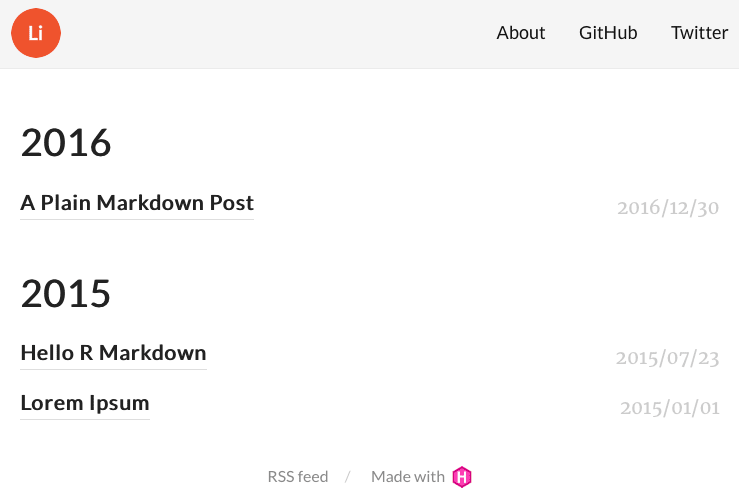
\includegraphics[width=0.9\linewidth]{images/lithium-theme} 

}

\caption{La página de inicio del nuevo sitio por defecto.}\label{fig:lithium}
\end{figure}

Tiene que saber tres conceptos más básicos para un sitio web basado en
Hugo:

\begin{enumerate}
\def\labelenumi{\arabic{enumi}.}
\item
  El archivo de configuración \texttt{config.toml}\index{config.toml},
  en el que puede especificar algunas configuraciones globales para su
  sitio. Incluso si no sabe qué es TOML en este momento (se presentará
  en el capítulo \ref{hugo}), aún podrá cambiar algunas configuraciones
  obvias. Por ejemplo, puede ver configuraciones como estas en
  \texttt{config.toml}:

\begin{Shaded}
\begin{Highlighting}[]
\NormalTok{baseurl }\OperatorTok{=} \StringTok{"/"}
\NormalTok{languageCode }\OperatorTok{=} \StringTok{"en-us"}
\NormalTok{title }\OperatorTok{=} \StringTok{"A Hugo website"}
\NormalTok{theme }\OperatorTok{=} \StringTok{"hugo-lithium-theme"}

\NormalTok{[[}\VariableTok{menu}\NormalTok{.}\AttributeTok{main}\NormalTok{]]}
\NormalTok{    name }\OperatorTok{=} \StringTok{"About"}
\NormalTok{    url }\OperatorTok{=} \StringTok{"/about/"}
\NormalTok{[[}\VariableTok{menu}\NormalTok{.}\AttributeTok{main}\NormalTok{]]}
\NormalTok{    name }\OperatorTok{=} \StringTok{"GitHub"}
\NormalTok{    url }\OperatorTok{=} \StringTok{"https://github.com/rstudio/blogdown"}
\NormalTok{[[}\VariableTok{menu}\NormalTok{.}\AttributeTok{main}\NormalTok{]]}
\NormalTok{    name }\OperatorTok{=} \StringTok{"Twitter"}
\NormalTok{    url }\OperatorTok{=} \StringTok{"https://twitter.com/rstudio"}
\end{Highlighting}
\end{Shaded}

  Puede cambiar el título de la página web, e.g.,
  \texttt{title\ =\ "Mi\ propia\ página\ web\ chévere"}, y actualizar
  las URL de GitHub y Twitter.\index{Directories}
\item
  El directorio de contenido (por defecto, \texttt{content/}). Aquí es
  donde usted escribe los archivos de origen R Markdown o Markdown para
  sus publicaciones y páginas. Bajo \texttt{content/} del sitio
  predeterminado, puede ver \texttt{about.md} y un
  directorio\texttt{post/} que contiene algunas publicaciones. La
  organización del directorio de contenido depende de usted. Puede tener
  archivos y directorios arbitrarios allí, según la estructura del sitio
  web que desee.
\item
  El directorio de publicación (por defecto, \texttt{public/}). Su sitio
  web se generará en este directorio, lo que significa que no necesita
  agregar manualmente ningún archivo a este directorio.\footnote{Ejecutando
    \texttt{serve\_site()} o \texttt{build\_site()}, los archivos se
    generarán y publicarán en su directorio de publicación
    automáticamente.} Por lo general, contiene una gran cantidad de
  archivos \texttt{*.html} y dependencias como \texttt{*.css},
  \texttt{*.js} e imágenes. Puede cargar todo en \texttt{public/} a
  cualquier servidor web que pueda publicar sitios web estáticos, y su
  sitio web estará en funcionamiento. Hay muchas opciones para publicar
  sitios web estáticos, y hablaremos más sobre ellos en el capítulo
  \ref{implementación} si no está familiarizado con la implementación de
  sitios web.
\end{enumerate}

Si está satisfecho con este tema predeterminado, ¡está básicamente listo
para comenzar a escribir y publicar su nuevo sitio web! Mostraremos cómo
usar otros temas en la sección \ref{otros-temas}. Sin embargo, tenga en
cuenta que un tema más complicado y elegante puede requerir que aprenda
más sobre todas las tecnologías subyacentes, como el lenguaje de
plantillas de Hugo, HTML, CSS y JavaScript.

\hypertarget{rstudio-ide}{%
\section{RStudio IDE}\label{rstudio-ide}}

Hay algunos complementos básicos de
RStudio\index{Complementos de RStudio} para facilitar la edición y la
vista previa de su sitio web, y puede encontrarlos en el menú ``Addins''
en la barra de herramientas de RStudio:

\begin{itemize}
\item
  ``Serve Site'': este complemento llama a
  \texttt{blogdown::serve\_site()} para presentar continuamente su sitio
  web localmente utilizando la tecnología LiveReload, para que pueda ver
  en vivo el sitio web. Puede seguir editando material para su sitio
  mientras lo está viendo, pero esta función bloqueará su consola de R
  de manera predeterminada, lo que significa que no podrá usar su
  consola de R una vez que inicie este servidor web local. Para
  desbloquear la consola, haga clic en el signo de stop rojo en la
  esquina superior derecha de la ventana de la consola. Si prefiere
  evitar este comportamiento por completo, establezca la opción
  \texttt{options(servr.daemon\ =\ TRUE)}, antes de hacer clic en este
  complemento o llame a la función \texttt{serve\_site()}, para que el
  servidor sea demonizado y no bloquee su consola de R.\^{} {[}Hemos
  oído de casos en los que el servidor demonizado bloquea R en Windows.
  Si tiene problemas con el servidor daemonizado, existen tres
  soluciones alternativas, y puede probar una de ellas: (1) instalar el
  paquete \textbf{later} a través de \texttt{install.packages("later")}
  y volver a iniciar el servidor; (2) use el servidor de Hugo (vea la
  sección \ref{livereload}); (3) llame \texttt{blogdown::serve\_site()}
  en una sesión de R separada, y puede obtener una vista previa de su
  sitio web en su navegador web, pero aún puede editar el sitio web en
  RStudio.{]}
\item
  ``New Post'': este complemento proporciona un cuadro de diálogo para
  que ingrese los metadatos de la publicación de su blog, incluidos el
  título, el autor, la fecha, etc. Ver la Figura \ref{fig:new-post} para
  un ejemplo. Este complemento realmente llama a la función
  \texttt{blogdown::new\_post()}, pero hace algunas cosas
  automáticamente:

  \begin{itemize}
  \item
    A medida que escribe el título de la publicación, generará un nombre
    de archivo para usted, y puede editarlo si no le gusta el generado
    automáticamente. De hecho, también puede usar este complemento para
    crear páginas normales en cualquier directorio bajo
    \texttt{content/}. Por ejemplo, si desea agregar una página de
    currículum, puede cambiar el nombre del archivo a \texttt{resume.md}
    del 'post/YYYY-mm-dd-resume.md` predeterminado.
  \item
    Puede seleccionar la fecha desde un widget de calendario
    proporcionado por Shiny.\footnote{Shiny es un paquete R para crear
      aplicaciones web interactivas usando R. Usando este complemento,
      el widget de calendario le permite ver un calendario interactivo
      por mes para seleccionar fechas. Este es un uso simple de Shiny,
      pero puede leer más acerca de las aplicaciones Shiny aquí:
      \url{https://shiny.rstudio.com}.}
  \item
    Esto escaneará las categorías y etiquetas de las publicaciones
    existentes, por lo que cuando quiera ingresar categorías o
    etiquetas, puede seleccionarlas de los menús desplegables o crear
    otras nuevas.
  \item
    Después de crear una nueva publicación, se abrirá automáticamente,
    por lo que puede comenzar a escribir el contenido de inmediato.
  \end{itemize}
\item
  ``Update Metadata'': Este complemento le permite actualizar los
  metadatos YAML de la publicación abierta actualmente. Ver la Figura
  @ref(fig: update-meta) para un ejemplo. La principal ventaja de este
  complemento es que puede seleccionar categorías y etiquetas de los
  menús desplegables en lugar de tener que recordarlas.
\end{itemize}

\begin{figure}

{\centering 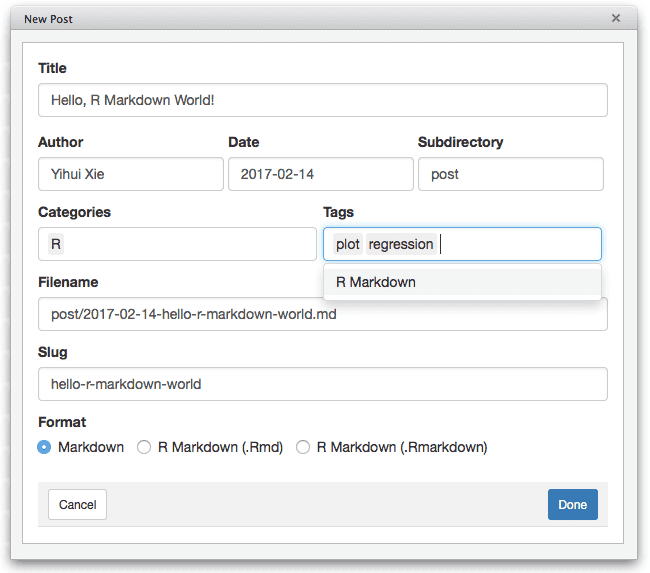
\includegraphics[width=0.8\linewidth]{images/new-post} 

}

\caption{Crear una nueva publicación usando el complemento de RStudio.}\label{fig:new-post}
\end{figure}

\begin{figure}

{\centering 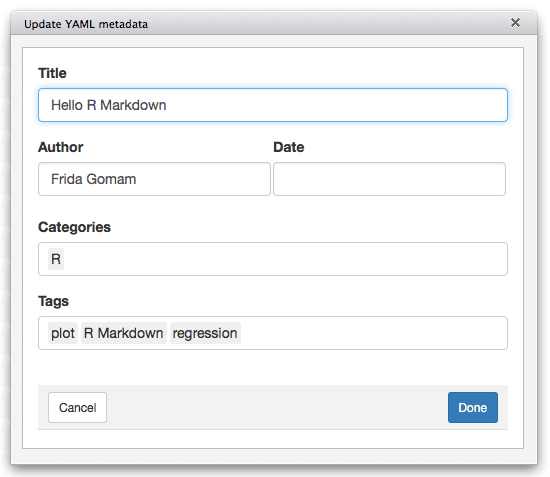
\includegraphics[width=0.7\linewidth]{images/update-meta} 

}

\caption{Actualizar los metadatos de una publicación existente usando el complemento de RStudio.}\label{fig:update-meta}
\end{figure}

Con estos complementos, rara vez deberá ejecutar los comandos en R
manualmente después de haber configurado su sitio web, ya que todas sus
publicaciones se compilarán automáticamente cada vez que cree una nueva
publicación o modifique una existente debido a la función LiveReload.

Si su versión de RStudio es por lo menos la v1.1.383,\footnote{Puede
  descargar todas las versiones del sitio oficial de RStudio incluyendo
  la v1.1.383 desde
  \url{https://www.rstudio.com/products/rstudio/download/}.} puede
actualmente crear un proyecto de página web directamente desde el menú
\texttt{File\ -\textgreater{}\ New\ Project\ -\textgreater{}\ New\ Directory}
(vea la Figura \ref{fig:new-project} y \ref{fig:blogdown-project}).

\begin{figure}

{\centering 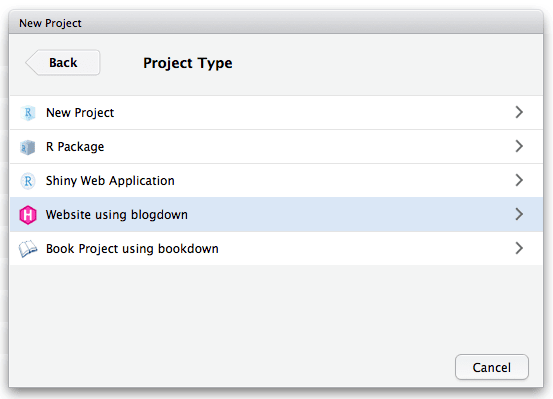
\includegraphics[width=0.8\linewidth]{images/new-project} 

}

\caption{Crear un nuevo proyecto de página web en RStudio.}\label{fig:new-project}
\end{figure}

\begin{figure}

{\centering 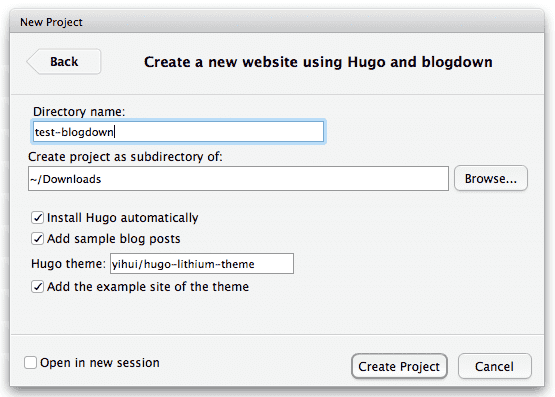
\includegraphics[width=0.8\linewidth]{images/blogdown-project} 

}

\caption{Crear un proyecto de página web basado en blogdown.}\label{fig:blogdown-project}
\end{figure}

Si su sitio web se creó utilizando la función
\texttt{blogdown::new\_site()} en lugar del menú de RStudio por primera
vez, puede salir de RStudio y volver a abrir el proyecto. Si accede al
menú \texttt{Tools\ -\textgreater{}\ Project\ Options}, su tipo de
proyecto debería ser ``Website'' como lo puede ver en la Figura
\ref{fig:project-options}.

Luego verá un panel en RStudio llamado ``Build'' y hay un botón ``Build
Website''. Al hacer clic en este botón, RStudio llamará a
\texttt{blogdown::build\_site\ ()} para construir el sitio web. Esto
generará automáticamente archivos en el directorio
\texttt{public/}.\footnote{O donde sea que esté ubicado su directorio de
  publicación. Es \texttt{public/} de forma predeterminada, pero se
  puede cambiar especificando \texttt{publishDir\ ="myNewDirectory"} en
  el archivo \texttt{config.toml}.} Si desea compilar el sitio web y
publicar los archivos de salida en \texttt{public/} manualmente, se
recomienda reiniciar su sesión de R y hacer clic en este botón ``Build
Website'' antes de publicar el sitio web, en lugar de publicar la
carpeta \texttt{public/} generada de forma continua y automática por
\texttt{blogdown::serve\_site()}, porque este último llama a
\texttt{blogdown::build\_site(local\ =\ TRUE)}, que tiene algunas
diferencias sutiles con \texttt{blogdown::build\_site(local\ =\ FALSE)}
(ver la sección \ref{local-preview} para más detalles).

Recomendamos mucho que desmarque la opción ``Preview site after
building'' en las opciones de proyecto de RStudio (Figura
\ref{fig:project-options}).\footnote{En caso de que se pregunte por qué:
  a menos que haya establecido la opción \texttt{relativeurls} a
  \texttt{true} en \texttt{config.toml}, requiere un servidor web para
  obtener una vista previa del sitio local, de lo contrario, incluso si
  puede ver la página de inicio de su sitio web en RStudio Viewer, la
  mayoría de los enlaces como los enlaces a archivos CSS y JavaScript
  son poco probables que funcionen. Cuando RStudio Viewer le muestra la
  vista previa, en realidad no ejecuta un servidor web.} También puede
desmarcar la opción ``Re-knit current preview when supporting files
change'', ya que esta opción no es realmente útil después de llamar a
\texttt{serve\_site()}.

\begin{figure}

{\centering 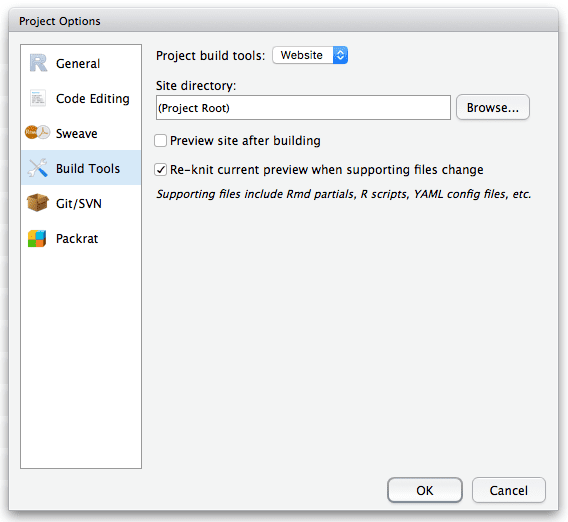
\includegraphics[width=0.8\linewidth]{images/project-options} 

}

\caption{Opciones de proyecto de RStudio.}\label{fig:project-options}
\end{figure}

\hypertarget{opciones-globales}{%
\section{\texorpdfstring{Opciones
globales\index{Global Options}}{Opciones globales}}\label{opciones-globales}}

Dependiendo de sus preferencias personales, puede establecer algunas
opciones globales antes de trabajar en su sitio web. Estas opciones se
deben configurar usando \texttt{options(name\ =\ value)}, y las opciones
disponibles actualmente se presentan en Table \ref{tab:global-options}.

\begin{table}

\caption{\label{tab:global-options}Opciones globales que afectan el comportamiento de blogdown.}
\centering
\begin{tabular}[t]{lll}
\toprule
Option name & Default & Meaning\\
\midrule
servr.daemon & FALSE & Si debe usar un servidor demonizado\\
blogdown.author &  & El autor por defecto de nuevas publicaciones\\
blogdown.ext & .md & Extensión por defecto de nuevas publicaciones\\
blogdown.subdir & post & Un subdirectorio bajo content/\\
blogdown.yaml.empty & TRUE & Preservar campos vacíos en YAML?\\
\bottomrule
\end{tabular}
\end{table}

Le recomendamos que configure estas opciones en su archivo de perfil de
inicio de R. Puede consultar la página de ayuda \texttt{?Rprofile} para
más detalles, y aquí hay una introducción simplificada. Un archivo de
perfil de inicio es básicamente un script en R que se ejecuta cuando se
inicia la sesión de R. Este es un lugar perfecto para establecer
opciones globales, por lo que no necesita escribir estas opciones
nuevamente cada vez que inicie una nueva sesión en R. Puede usar un
archivo de perfil global \texttt{\textasciitilde{}/.Rprofile},\footnote{La
  tilde \texttt{\textasciitilde{}} indica el directorio principal en su
  sistema.} O un archivo por proyecto \texttt{.Rprofile} en el
directorio raíz de su proyecto de RStudio. El primero se aplicará a
todas las sesiones de R que inicie, a menos que haya proporcionado el
último para anularlo. La forma más fácil de crear un archivo de este
tipo es usar \texttt{file.edit()} en RStudio, por ejemplo,

\begin{Shaded}
\begin{Highlighting}[]
\KeywordTok{file.edit}\NormalTok{(}\StringTok{'~/.Rprofile'}\NormalTok{)}
\CommentTok{# o file.edit('.Rprofile')}
\end{Highlighting}
\end{Shaded}

Supongamos que siempre prefiere el servidor demonizado y quiere que el
autor de las nuevas publicaciones sea ``John Doe'' de manera
predeterminada. Puede establecer estas opciones en el archivo de perfil:

\begin{Shaded}
\begin{Highlighting}[]
\KeywordTok{options}\NormalTok{(}\DataTypeTok{servr.daemon =} \OtherTok{TRUE}\NormalTok{, }\DataTypeTok{blogdown.author =} \StringTok{'John Doe'}\NormalTok{)}
\end{Highlighting}
\end{Shaded}

Una buena consecuencia de establecer estas opciones es que cuando usa el
complemento de RStudio ``New post'', los campos ``Author'',
``Subdirectory'' y ``Format'' se completarán automáticamente, por lo que
no tendrá que manipularlos todas las veces a menos que desea cambiar los
valores predeterminados (ocasionalmente).

R solo lee un archivo de perfil de inicio. Por ejemplo, si tiene un
\texttt{.Rprofile} en el directorio actual y un
\texttt{\textasciitilde{}/.Rprofile} global, solo el anterior se
ejecutará cuando R se inicie desde el directorio actual. Esto puede
hacer que sea inconveniente para varios autores que colaboran en el
mismo proyecto de un sitio web, ya que no puede establecer opciones
específicas del autor. En particular, no es posible establecer la opción
\texttt{blogdown.author} en un solo \texttt{.Rprofile}, porque esta
opción debería ser diferente para diferentes autores. Una solución
consiste en establecer opciones comunes en \texttt{.Rprofile} bajo del
directorio raíz del proyecto del sitio web, y también ejecutar el
\texttt{\textasciitilde{}/.Rprofile} global si existe. Las opciones
específicas del autor se pueden establecer en el
\texttt{\textasciitilde{}/.Rprofile} global en la computadora de cada
autor.

\begin{Shaded}
\begin{Highlighting}[]
\CommentTok{# en el .Rprofile del proyecto de la página web}
\ControlFlowTok{if}\NormalTok{ (}\KeywordTok{file.exists}\NormalTok{(}\StringTok{'~/.Rprofile'}\NormalTok{)) \{}
\NormalTok{  base}\OperatorTok{::}\KeywordTok{sys.source}\NormalTok{(}\StringTok{'~/.Rprofile'}\NormalTok{, }\DataTypeTok{envir =} \KeywordTok{environment}\NormalTok{())}
\NormalTok{\}}
\CommentTok{# luego configure options(blogdown.author = 'Your Name') en ~/.Rprofile}
\end{Highlighting}
\end{Shaded}

\hypertarget{output-format}{%
\section{R Markdown vs.~Markdown}\label{output-format}}

Si no está familiarizado con R Markdown \index{R Markdown}, consulte el
Apéndice \ref{r-markdown} para obtener un tutorial rápido. Cuando crea
una nueva publicación, debe decidir si desea usar R Markdown o Markdown
simple \index{Markdown}, como puede ver en Figure \ref{fig:new-post}.
Las principales diferencias son:

\begin{enumerate}
\def\labelenumi{\arabic{enumi}.}
\item
  No puede ejecutar ningún código en R en un documento de Markdown
  simple, mientras que en un documento de Markdown R, puede incrustar
  fragmentos de código R
  (\texttt{\textasciigrave{}\textasciigrave{}\textasciigrave{}\{r\}}).
  Sin embargo, aún puede incrustar código de R en Markdown simple usando
  la sintaxis para bloques de código delimitados
  \texttt{\textasciigrave{}\textasciigrave{}\textasciigrave{}r}(tenga en
  cuenta que no hay llaves \texttt{\{\}}). Tales bloques de código no se
  ejecutarán y pueden ser adecuados para propósitos de demostración
  pura. A continuación se muestra un ejemplo de un fragmento de código
  de R en R Markdown:

\begin{Shaded}
\begin{Highlighting}[]
\NormalTok{```\{r cool-plot, fig.width='80%', fig.cap='A cool plot.'\}}
\NormalTok{plot(cars, pch = 20)  # no es muy chévere}
\NormalTok{```}
\end{Highlighting}
\end{Shaded}

  Y aquí hay un ejemplo de un bloque de código de R en Markdown simple:

\begin{Shaded}
\begin{Highlighting}[]
\NormalTok{```r}
\NormalTok{1 + 1  # no ejecutada}
\NormalTok{```}
\end{Highlighting}
\end{Shaded}
\item
  Una publicación en Markdown simple es ejecutada en HTML a través de
  \href{https://gohugo.io/overview/configuration/}{Blackfriday}
  \index{Blackfriday}(un paquete escrito en lenguaje Go y adoptado por
  Hugo). Un documento R Markdown se compila a través de los paquetes
  \textbf{rmarkdown}, \textbf{bookdown}, y Pandoc\index{Pandoc}, lo que
  significa que puede usar la mayoría de las características de
  \href{http://pandoc.org/MANUAL.html\#pandocs-markdown}{Markdown de
  Pandoc} y
  \href{https://bookdown.org/yihui/bookdown/components.html}{extensiones
  de Markdown para \textbf{bookdown}} en \textbf{blogdown}. Si usa R
  Markdown \citep{R-rmarkdown} con \textbf{blogdown}, le recomendamos
  que lea la documentación de Pandoc y \textbf{bookdown} al menos una
  vez para conocer todas las características posibles. No repetiremos
  los detalles en este libro, pero enumeraremos las características
  brevemente a continuación, que también se muestran en el sitio web de
  ejemplo: \url{https://blogdown-demo.rbind.io}.

  \begin{itemize}
  \item
    Formateo en línea: texto en \texttt{\_italica\_} /
    \texttt{**negrita**} y
    \texttt{\textasciigrave{}código\ en\ línea\textasciigrave{}}.
  \item
    Elementos en línea: subíndices (e.g.,
    \texttt{H\textasciitilde{}2\textasciitilde{}0}) y superíndices
    (e.g., \texttt{R\^{}2\^{}}); links (\texttt{{[}texto{]}(url)}) e
    imágenes \texttt{!{[}título{]}(url)}; notas al pie
    \texttt{texto\^{}{[}nota\ al\ pie{]}}.
  \item
    Elementos de nivel bloque: párrafos; encabezados de sección
    numerados y no numerados; listas ordenadas y no ordenadas; citas en
    bloque; bloques de código; tablas; reglas horizontales.
  \item
    Expresiones matemáticas y ecuaciones.
  \item
    Teoremas y demostraciones.
  \item
    Bloques de código en R que se pueden usar para producir salida de
    texto (incluidas tablas) y gráficos. Tenga en cuenta que las
    ecuaciones, teoremas, tablas y figuras se pueden numerar y
    referenciadas cruzadamente.
  \item
    Citas y bibliografía.
  \item
    HTML widgets, y aplicaciones en Shiny incrustadas mediante
    \texttt{\textless{}iframe\textgreater{}}.
  \end{itemize}
\end{enumerate}

Hay muchas diferencias en la sintaxis entre el Markdown de Blackfriday y
el Markdown de Pandoc. Por ejemplo, puede escribir una lista de tareas
con Blackfriday, pero no con Pandoc:

\begin{Shaded}
\begin{Highlighting}[]
\NormalTok{- }\FloatTok{[x] Escribir un paquete en R.}
\FloatTok{- [ ] Escribir un libro.}
\FloatTok{- [ ] ...}
\FloatTok{- [ ] Beneficio!}
\end{Highlighting}
\end{Shaded}

Del mismo modo, Blackfriday no admite matemática en LaTeX y Pandoc sí.
Hemos agregado el soporte \href{https://www.mathjax.org/\#docs}{MathJax}
\index {MathJax} al tema predeterminado
(\href{https://github.com/yihui/hugo-lithium-theme}{hugo-lithium-theme}
en \textbf{blogdown} para compilar matemática en LaTeX en páginas HTML,
pero hay una advertencia para las publicaciones simples de Markdown:
debe incluir expresiones matemáticas en línea con un par de comillas
\texttt{\textasciigrave{}\$math\$\textasciigrave{}}, por ejemplo,
\texttt{\textasciigrave{}\$S\_n\ =\ \textbackslash{}\ um\_\{i=1\}\^{}n\ X\_i\$\textasciigrave{}}.
Del mismo modo, las expresiones matemáticas del estilo de visualización
deben escribirse en
\texttt{\textasciigrave{}\$\$math\$\$\textasciigrave{}}. Para las
publicaciones de R Markdown, puede usar \texttt{\$math\$} para
expresiones matemáticas en línea, y \texttt{\$\$math\$\$} para
expresiones de estilo de visualización.\footnote{El motivo por el que
  necesitamos los respaldos para documentos de Markdown simples es que
  tenemos que evitar que Blackfriday interprete el código LaTeX como
  Markdown. Las comillas asegurarán que el contenido interno no se
  traduzca como Markdown a HTML, por ejemplo,
  \texttt{\textasciigrave{}\$\$x\ *y*\ z\$\$\textasciigrave{}} se
  convertirá en
  \texttt{\textless{}code\textgreater{}\ \$\$x\ *y*\ z\$\$\textless{}/code\textgreater{}}.
  Sin las comillas, se convertirá en
  \texttt{\$\$x\ \textless{}em\textgreater{}y\textless{}/em\textgreater{}\ z\$\$},
  que no es una expresión matemática en LaTeX válida para MathJax.
  Problemas similares pueden surgir cuando tenga otros caracteres
  especiales como guiones bajos en sus expresiones matemáticas.}

Si considera que es un dolor tener que recordar las diferencias entre R
Markdown y Markdown, una opción conservadora es usar siempre R Markdown,
incluso si su documento no contiene ningún fragmento de código en R.
Markdown de Pandoc es mucho más rico que Blackfriday, y solo hay un
pequeño número de características no disponibles en Pandoc pero
presentes en Blackfriday. Las principales desventajas de usar R Markdown
son:

\begin{enumerate}
\def\labelenumi{\arabic{enumi}.}
\item
  Puede sacrificar algo de velocidad en la renderización del sitio web,
  pero esto puede no ser notorio debido a un mecanismo de almacenamiento
  en caché en \textbf{blogdown} (lea más sobre esto en la sección
  \ref{local-preview}). Hugo es muy rápido cuando procesa archivos de
  Markdown simples, y típicamente debería tomar menos de un segundo para
  renderizar unos cientos de archivos de Markdown.
\item
  Tendrá algunos archivos HTML intermedios en el directorio fuente de su
  sitio web, porque \textbf{blogdown} tiene que llamar a
  \textbf{rmarkdown} para renderizar previamente los archivos
  \texttt{*.Rmd} \texttt{*.html}. También tendrá carpetas intermedias
  para las figuras (\texttt{*\_files/}) y la memoria caché
  (\texttt{*\_cache/}) si tiene una salida de trazado en fragmentos de
  código en R o ha habilitado el almacenamiento en cache de
  \textbf{knitr}. A menos que le importe mucho la ``limpieza'' del
  repositorio fuente de su sitio web (especialmente cuando usa una
  herramienta de control de versiones como GIT), estos archivos
  intermedios no deberían importar.
\end{enumerate}

En este libro, generalmente nos referimos a los archivos \texttt{.Rmd}
cuando decimos ``Documentos de R Markdown'', que se compilan a
\texttt{.html} de forma predeterminada. Sin embargo, hay otro tipo de
documento de R Markdown con la extensión de nombre de archivo
\texttt{.Rmarkdown}. Dichos documentos de R Markdown se compilan para
los documentos Markdown con la extensión \texttt{.markdown}, que serán
procesados por Hugo en lugar de por Pandoc. Hay dos limitaciones
principales de usar \texttt{.Rmarkdown} en comparación con\texttt{.Rmd}:

\begin{itemize}
\item
  No puede usar las funciones de reducción solo compatibles con Pandoc,
  como las citas. Las expresiones matemáticas solo funcionan si ha
  instalado el paquete \textbf{xaringan} \citep{R-xaringan} y ha
  aplicado la solución de JavaScript mencionada en la sección
  \ref{javascript}.
\item
  Los widgets HTML no son compatibles.
\end{itemize}

La principal ventaja de usar \texttt{.Rmarkdown} es que los archivos de
salida son más limpios porque son archivos Markdown. Puede ser más fácil
para usted leer la salida de sus publicaciones sin mirar las páginas web
reales renderizadas. Esto puede ser particularmente útil al revisar los
pull requests de GitHub. Tenga en cuenta que las tablas, figuras,
ecuaciones y teoremas numerados también son compatibles. No puede usar
directamente la sintaxis de Markdown en las leyendas de tabla o figura,
pero puede usar referencias de texto como una solución alternativa
(consulte la documentación de \textbf{bookdown}).

Para cualquier documento de R Markdown (no específico de
\textbf{blogdown}), debe especificar un formato de salida. Hay muchos
posibles \href{http://rmarkdown.rstudio.com/lesson-9.html}{formatos de
salida} en el paquete \textbf{rmarkdown} (como \texttt{html\_document} y
\texttt{pdf\_document}) y otros paquetes de extensión (tales como
\texttt{tufte::tufte\_html} y \texttt{bookdown::gitbook}). Por supuesto,
el formato de salida para los sitios web debe ser HTML. Hemos
proporcionado una función de formato de salida
\texttt{blogdown::html\_page} en \textbf{blogdown}, y todos los archivos
R Markdown se renderizan con este formato. Se basa en el formato de
salida \texttt{bookdown::html\_document2}, lo que significa que ha
heredado muchas características de \textbf{bookdown} además de las
características en Pandoc. Por ejemplo, puede numerar y hacer
referencias cruzadas de ecuaciones matemáticas, figuras, tablas y
teoremas, etc. Consulte el Capítulo 2 del libro \textbf{bookdown}
\citep{xie2016} para obtener más detalles sobre la sintaxis.

Note que el formato de salida \texttt{bookdown::html\_document2} a su
vez hereda de \texttt{rmarkdown::html\_document}, entonces necesita ver
la página de ayuda \texttt{?rmarkdown::html\_document} para todas las
opciones posibles para el formato \texttt{blogdown::html\_page}. Si
desea cambiar los valores predeterminados de las opciones de este
formato de salida, puede agregar un campo \texttt{output} a sus
metadatos YAML. Por ejemplo, podemos agregar una tabla de contenido a
una página, establecer el ancho de la figura en 6 pulgadas y usar el
dispositivo \texttt{svg} para los gráficos estableciendo estas opciones
en YAML:

\begin{Shaded}
\begin{Highlighting}[]
\OtherTok{---}
\FunctionTok{title:}\AttributeTok{ }\StringTok{"Mi grandiosa publicación"}
\StringTok{author: "}\ErrorTok{John Doe"}
\FunctionTok{date:}\AttributeTok{ }\StringTok{"2017-02-14"}
\FunctionTok{output:}
  \FunctionTok{blogdown:}\AttributeTok{:html_page:}
    \FunctionTok{toc:}\AttributeTok{ true}
    \FunctionTok{fig_width:}\AttributeTok{ 6}
    \FunctionTok{dev:}\AttributeTok{ }\StringTok{"svg"}
\OtherTok{---}
\end{Highlighting}
\end{Shaded}

Para establecer opciones para \texttt{blogdown::html\_page()}
globalmente (es decir, aplicar ciertas opciones a todos los archivos
Rmd), puede crear un archivo \texttt{\_output.yml} en el directorio raíz
de su sitio web. Este archivo YAML debe contener el formato de salida
directamente (no coloque el formato de salida bajo la opción
\texttt{output}), por ejemplo,

\begin{Shaded}
\begin{Highlighting}[]
\FunctionTok{blogdown:}\AttributeTok{:html_page:}
  \FunctionTok{toc:}\AttributeTok{ true}
  \FunctionTok{fig_width:}\AttributeTok{ 6}
  \FunctionTok{dev:}\AttributeTok{ }\StringTok{"svg"}
\end{Highlighting}
\end{Shaded}

Por el momento, no todas las funciones de
\texttt{rmarkdown::html\_document} son compatibles con
\textbf{blogdown}, como \texttt{df\_print},
\texttt{code\_folding},\texttt{code\_download}, etc.

Si su trozo de código tiene salida de gráficos, le recomendamos que
evite caracteres especiales como espacios en la etiqueta de fragmentos.
Lo ideal es que solo use caracteres alfanuméricos y guiones, por
ejemplo,
\texttt{\textasciigrave{}\textasciigrave{}\textasciigrave{}\{r,\ my-label\}}
en lugar de
\texttt{\textasciigrave{}\textasciigrave{}\textasciigrave{}\{r,\ my\ label\}}.

No se recomienda cambiar las opciones \textbf{knitr} chunk
\texttt{fig.path} o \texttt{cache.path} en R Markdown. Los valores
predeterminados de estas opciones funcionan mejor con \textbf{blogdown}.
Lea la sección \ref{dep-path} para conocer los motivos técnicos, si lo
prefiere.

Si está trabajando en una publicación de R Markdown, pero no quiere que
\textbf{blogdown} la compile, puede cambiar temporalmente su extensión
de nombre de archivo de \texttt{.Rmd} a otra extensión desconocida como
\texttt{.Rmkd}.

\hypertarget{otros-temas}{%
\section{Otros temas}\label{otros-temas}}

En Hugo, los temas \index{Temas} controlan toda la apariencia y
funcionalidad de su sitio. Entonces, si le importa mucho el aspecto de
su sitio web, probablemente pasará bastante tiempo al principio buscando
un tema de Hugo que le guste de la colección que figura en
\url{http://themes.gohugo.io}. Tenga en cuenta que no todos los temas se
han probado en \textbf{blogdown}. Si encuentra que un determinado tema
no funciona bien con \textbf{blogdown}, puede informar a
\url{https://github.com/rstudio/blogdown/issues}, e intentaremos
investigar el motivo, pero puede ser una cuestión de tiempo aprender y
comprender cómo funciona un nuevo tema, por lo que le recomendamos que
aprenda más acerca de Hugo por su cuenta antes de preguntar, y también
alentamos a los usuarios a ayudarse mutuamente allí.

Después de haber encontrado un tema satisfactorio, debe averiguar su
nombre de usuario y el nombre del repositorio de GitHub,\footnote{Para
  la mayoría de los temas, puede encontrar esto navegando al tema de su
  elección desde \url{http://themes.gohugo.io} y luego haciendo clic en
  \texttt{Homepage}.} luego instale el tema a través
de\index{blogdown::install\_theme()}
\texttt{blogdown::install\_theme()}, o simplemente cree un nuevo sitio
bajo otro directorio nuevo y pase el nombre del repositorio de GitHub al
argumento \texttt{theme} de \texttt{new\_site()}. Recomendamos que use
el segundo enfoque, porque los temas de Hugo podrían ser muy complicados
y el uso de cada tema puede ser muy diferente y muy dependiente del
\texttt{config.toml}. Si instala un tema con \texttt{install\_theme()}
en lugar de \texttt{new\_site\ ()}, deberá crear manualmente el archivo
\texttt{config.toml} en el directorio raíz de su sitio web para que
coincida con el tema recién instalado.\footnote{Una solución
  alternativa, si usó \texttt{install\_theme()} y establece el argumento
  \texttt{theme\_example} en TRUE, entonces puede acceder a un archivo
  \texttt{config.toml} de ejemplo. En el directorio \texttt{themes/},
  vaya al archivo del tema que acaba de descargar y busque
  \texttt{exampleSite/config.toml}. Este archivo puede copiarse en su
  directorio raíz (para reemplazar el archivo \texttt{config.toml} de su
  tema original) o usarse como una plantilla para escribir correctamente
  un nuevo archivo \texttt{config.toml} para su nuevo tema.}

\begin{Shaded}
\begin{Highlighting}[]
\CommentTok{# por ejemplo, cree un sitio nuevo con el tema academic}
\NormalTok{blogdown}\OperatorTok{::}\KeywordTok{new_site}\NormalTok{(}\DataTypeTok{theme =} \StringTok{'gcushen/hugo-academic'}\NormalTok{)}
\end{Highlighting}
\end{Shaded}

Para ahorrarle tiempo, enumeramos algunos temas a continuación que
coinciden con nuestro gusto:

\begin{itemize}
\item
  Temas Simples/mínimos:
  \href{https://github.com/yihui/hugo-xmin}{XMin,}
  \href{https://github.com/road2stat/hugo-tanka}{Tanka,}
  \href{https://github.com/AlexFinn/simple-a}{simple-a,} and
  \href{https://github.com/jbub/ghostwriter}{ghostwriter.}
\item
  Temas sofisticados:
  \href{https://github.com/gcushen/hugo-academic}{hugo-academic}
  (fuertemente recomendado para usuarios de la academia),
  \href{https://github.com/kakawait/hugo-tranquilpeak-theme}{hugo-tranquilpeak-theme,}
  \href{https://github.com/kishaningithub/hugo-creative-portfolio-theme}{hugo-creative-portfolio-theme,}
  and
  \href{https://github.com/devcows/hugo-universal-theme}{hugo-universal-theme.}
\item
  Temas que contienen multimedia: Si está interesado en agregar
  contenido multimedia a su sitio (como archivos de audio de un
  podcast), el tema
  \href{https://github.com/mattstratton/castanet}{castanet} proporciona
  un excelente marco adaptado para esta aplicación. Un ejemplo de un
  sitio que usa \textbf{blogdown} con el tema castanet es
  \href{https://www.r-podcast.org}{R-Podcast}
\end{itemize}

Si no entiende HTML, CSS o JavaScript, y no tiene experiencia con los
temas o plantillas de Hugo, puede tardar unos 10 minutos en comenzar a
usar su nuevo sitio web, ya que debe aceptar todo lo que le ofrecen
(como el tema predeterminado); Si tiene el conocimiento y la experiencia
(y desea personalizar su sitio al máximo), puede tardar varios días en
comenzar. Hugo es realmente poderoso. Tenga cuidado con el poder.

Otra cosa a tener en cuenta es que cuanto más esfuerzo hagas en un tema
complicado, más difícil será cambiar a otros temas en el futuro, porque
es posible que haya personalizado muchas cosas que no son fáciles de
transferir a otro tema. Por lo tanto, pregúntese seriamente: ``¿Me gusta
tanto este tema tan elegante que definitivamente no lo cambiaré en los
próximos años?''.

\begin{quote}
Si elige cavar un hoyo bastante profundo, algún día no tendrá más
remedio que seguir cavando, incluso con lágrimas.

\VA{--- Liyun Chen\footnote{Traducido de su weibo Chino:
  \url{http://weibo.com/1406511850/Dhrb4toHc} (no puede ver esta página
  a menos que haya iniciado sesión).}}{}
\end{quote}

\hypertarget{workflow}{%
\section{Un flujo de trabajo recomendado}\label{workflow}}

Hay muchas maneras de comenzar a construir un sitio web y presentarlo.
Debido a la gran cantidad de tecnologías que necesita aprender para
comprender completamente cómo funciona un sitio web, nos gustaría
recomendar un flujo de trabajo a los principiantes, por lo que es de
esperar que no necesiten digerir el resto de este libro. Definitivamente
este no es el flujo de trabajo más óptimo, pero requiere que conozca la
menor cantidad de detalles técnicos.

Para comenzar un nuevo sitio web:

\begin{enumerate}
\def\labelenumi{\arabic{enumi}.}
\item
  Elija cuidadosamente un tema en \url{http://themes.gohugo.io}, y
  encuentre el enlace a su repositorio GitHub, que tiene la forma
  \texttt{https://github.com/user/repo}.
\item
  Cree un nuevo proyecto en RStudio y escriba el código
  \texttt{blogdown::new\_site\ (theme\ =\ \textquotesingle{}user/repo\textquotesingle{})}
  en la consola R, donde \texttt{user/repo} proviene del enlace en el
  paso 1.
\item
  Juegue con el nuevo sitio por un tiempo y si no le gusta, puede
  repetir los pasos anteriores, de lo contrario edite las opciones en
  \texttt{config.toml}. Si no comprende ciertas opciones, vaya a la
  documentación del tema, que a menudo es la página README del
  repositorio de GitHub. No todas las opciones tienen que ser cambiadas.
\end{enumerate}

Para editar una página web:

\begin{enumerate}
\def\labelenumi{\arabic{enumi}.}
\item
  Establezca \texttt{options(servr.daemon\ =\ TRUE)} a menos que ya lo
  haya configurado en \texttt{.Rprofile}. Si esta opción no funciona
  para usted (por ejemplo, bloquea su sesión en R), consulte la sección
  \ref{opciones-globales} para obtener una solución alternativa.
\item
  Haga clic en el complemento de RStudio ``Serve Site'' para obtener una
  vista previa del sitio en RStudio Viewer. Esto solo debe hacerse una
  vez cada vez que abra el proyecto RStudio o reinicie su sesión en R.
  No haga clic en el botón knit en la barra de herramientas de RStudio.
\item
  Use el complemento ``New Post'' para crear una nueva publicación o
  página, luego empiece a escribir el contenido.
\item
  Use el complemento ``Update Metadata'' para modificar los metadatos
  del YAML, si es necesario.
\end{enumerate}

Para publicar un sitio web, si no está familiarizado con GIT o GitHub:

\begin{enumerate}
\def\labelenumi{\arabic{enumi}.}
\item
  Reinicie la sesión de R, y ejecute \texttt{blogdown::hugo\_build()}.
  Debería obtener un directorio \texttt{public/} bajo el directorio raiz
  de su proyecto.
\item
  Inicie sesión en\index{Netlify} \url{https://www.netlify.com} (puede
  usar una cuenta de GitHub, si la tiene). Si esta es la primera vez que
  publica este sitio web, puede crear un sitio nuevo; de lo contrario,
  puede actualizar el sitio existente que creó la última vez. Puede
  arrastrar y soltar la carpeta \texttt{public/} desde su visor de
  archivos al área indicada en la página web de Netlify, donde dice
  ``Drag a folder with a static site here''.
\item
  Espere unos segundos para que Netlify despliegue los archivos y le
  asignará un subdominio aleatorio de la forma
  \texttt{random-word-12345.netlify.com}. Puede (y debería) cambiar este
  subdominio aleatorio a uno más significativo si todavía está
  disponible.
\end{enumerate}

Puede ser mucho más fácil publicar un sitio web si está familiarizado
con GIT y GitHub. Recomendamos que cree un nuevo sitio en Netlify desde
su repositorio de GitHub que contenga los archivos fuente de su sitio
web, para que pueda disfrutar los beneficios de la implementación
continua en lugar de cargar manualmente la carpeta \texttt{public/} cada
vez. Con este enfoque, no es necesario ejecutar
\texttt{blogdown::hugo\_build()} localmente, ya que el sitio web se
puede construir en Netlify a través de Hugo. Consulte el capítulo
\ref{implementación} para obtener más información.

\hypertarget{hugo}{%
\chapter{Hugo}\label{hugo}}

En este capítulo, presentaremos brevemente\index{Hugo} Hugo
(\url{https://gohugo.io}), el generador de sitios estáticos en el que se
basa \textbf{blogdown}. Este capítulo no pretende reemplazar la
documentación oficial de Hugo, sino proporcionar una guía para aquellos
que recién están comenzando con Hugo. En caso de duda, consulte la
documentación oficial de Hugo.

\hypertarget{static-sites}{%
\section{Sitios estáticos y Hugo}\label{static-sites}}

Un sitio estático\index{Sitio estático} a menudo consiste en archivos
HTML (con dependencias externas opcionales como imágenes y bibliotecas
de JavaScript), y el servidor web envía exactamente el mismo contenido
al navegador web sin importar quién visita las páginas web. No hay
computación dinámica en el servidor cuando se solicita una página. En
contraste, un sitio dinámico se basa en un lenguaje del lado del
servidor para hacer cierta informática y envía contenido potencialmente
diferente dependiendo de las diferentes condiciones. Un lenguaje común
es PHP, y un ejemplo típico de un sitio dinámico es un foro web. Por
ejemplo, cada usuario tiene una página de perfil, pero generalmente esto
no significa que el servidor haya almacenado una página de perfil HTML
diferente para cada usuario. En cambio, el servidor obtendrá los datos
del usuario de una base de datos y renderizará la página de perfil de
forma dinámica.

Para un sitio estático, cada URL que visita a menudo tiene un archivo
HTML correspondiente almacenado en el servidor, por lo que no es
necesario calcular nada antes de presentar el archivo a los visitantes.
Esto significa que los sitios estáticos tienden a ser más rápidos en
tiempo de respuesta que los sitios dinámicos, y también son mucho más
fáciles de implementar, ya que la implementación simplemente significa
copiar archivos estáticos a un servidor. Un sitio dinámico a menudo se
basa en bases de datos, y tendrá que instalar más paquetes de software
para presentar un sitio dinámico. Para obtener más ventajas de los
sitios estáticos, lea la
\href{https://gohugo.io/overview/introduction/}{introducción} en el
sitio web de Hugo.

Existen muchos generadores de sitios estáticos existentes, incluyendo
Hugo, \href{http://jekyllrb.com}{Jekyll,} y
\href{https://hexo.io}{Hexo,} etc. La mayoría de ellos puede construir
sitios web de propósito general, pero a menudo se utilizan para
construir blogs.

Amamos a Hugo por muchas razones, pero hay algunas que se destacan. A
diferencia de otros generadores de sitios estáticos, la instalación de
Hugo es muy simple porque proporciona un único archivo ejecutable sin
dependencias para la mayoría de los sistemas operativos (consulte la
sección \ref{instalación}). También se diseñó para procesar cientos de
páginas de contenido más rápido que los generadores de sitios estáticos
comparables y, según los informes, puede presentar una página en
aproximadamente 1 milisegundo. Por último, la comunidad de usuarios de
Hugo es muy activa tanto en el \href{https://discuss.gohugo.io}{foro de
discusión de Hugo} y en los
\href{https://github.com/gohugoio/hugo/issues}{issues de GitHub.}

Aunque creemos que Hugo es un fantástico generador de sitios estáticos,
en realidad hay una única característica importante que falta: el
soporte para R Markdown. Ese es básicamente el objetivo del paquete
\textbf{blogdown}.\footnote{Otra motivación fue una manera más fácil de
  crear nuevas páginas o publicaciones. Los generadores de sitios
  estáticos a menudo proporcionan comandos para crear nuevas
  publicaciones, pero a menudo tiene que abrir y modificar el nuevo
  archivo creado a mano después de usar estos comandos. Estaba muy
  frustrado por esto, porque estaba buscando una interfaz gráfica de
  usuario donde simplemente pudiera completar el título, el autor, la
  fecha y otra información sobre una página, luego poder comenzar a
  escribir el contenido de inmediato. Es por eso que proporcioné el
  complemento de RStudio ``New Post'' y la función
  \texttt{blogdown::new\_post()}. En los últimos años, lo odié cada vez
  que estaba a punto de crear una nueva publicación, ya sea a mano o a
  través de la línea de comandos de Jekyll. Finalmente, me volví adicto
  a los blogs una vez que terminé el complemento de RStudio.} Esta
función faltante significa que no puede generar resultados fácilmente
usando el código de R en sus páginas web, ya que solo puede usar
documentos estáticos de Markdown. Además, el motor de Markdown
predeterminado de Hugo es ``Blackfriday'', que es menos poderoso que
Pandoc.\footnote{El soporte de Pandoc se ha agregado en un pull request
  de Hugo: \url{https://github.com/gohugoio/hugo/pull/4060}. Sin
  embargo, creo que el soporte es bastante limitado, y le recomiendo que
  use el formato R Markdown, porque con el soporte oficial de Pandoc en
  Hugo, no puede personalizar las opciones de la línea de comandos de
  Pandoc, la renderización no está en caché (podría ser lento), y no
  podrá usar ninguna extensión de Markdown del paquete \textbf{bookdown}
  (como la numeración de los títulos de las figuras).}

Hugo usa una estructura especial de archivos y carpetas para crear su
sitio web (Figura \ref{fig:folders}). El resto de este capítulo brindará
más detalles sobre los siguientes archivos y carpetas:

\begin{itemize}
\tightlist
\item
  \texttt{config.toml}
\item
  \texttt{content/}
\item
  \texttt{static/}
\item
  \texttt{themes/}
\item
  \texttt{layouts/}
\end{itemize}




\begin{figure}

{\centering 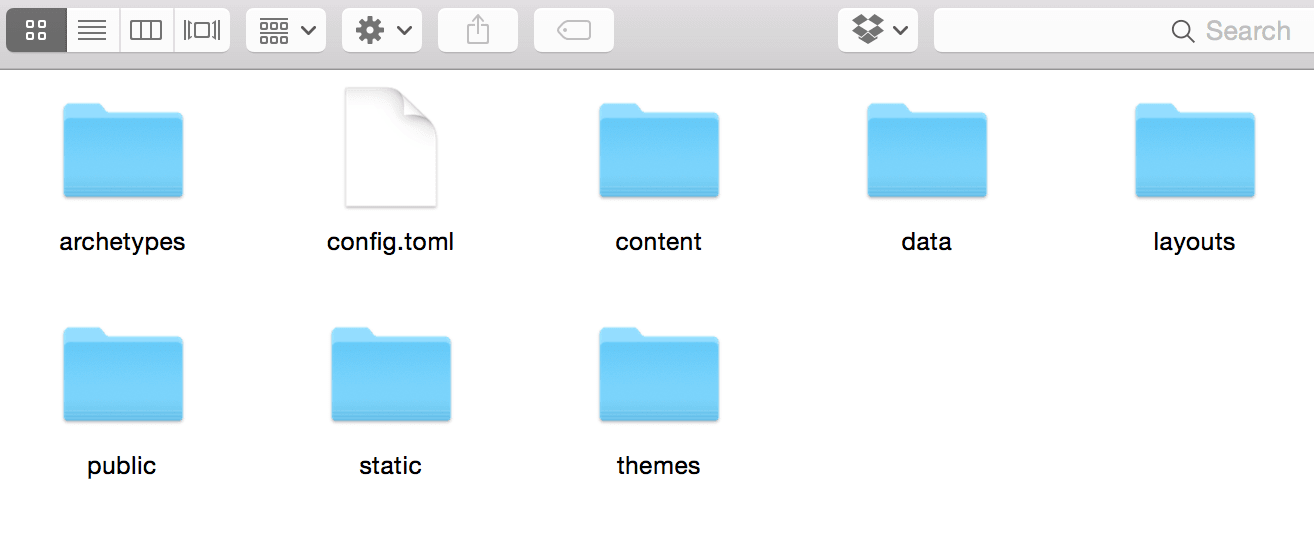
\includegraphics[width=1\linewidth]{images/folder-structure} 

}

\caption{Posibles archivos y carpetas creados cuando crea un nuevo
sitio usando \textbf{blogdown}.}\label{fig:folders}
\end{figure}

\hypertarget{configuracion}{%
\section{Configuración}\label{configuracion}}

El primer archivo que puede ver es el archivo
configuration\index{config.toml} o \texttt{config} en su directorio
raíz, en el que puede establecer configuraciones globales de su sitio.
Puede contener opciones como el título y la descripción de su sitio, así
como otras opciones globales como enlaces a sus redes sociales, el menú
de navegación y la URL base de su sitio web.

Al generar su sitio, Hugo buscará primero un archivo llamado
\texttt{config.toml}. Si no puede encontrar uno, continuará buscando
\texttt{config.yaml}.\footnote{Hugo también admite \texttt{config.json},
  pero \textbf{blogdown} no lo admite, por lo que no recomendamos que lo
  use.} Como la mayoría de los temas de Hugo contienen sitios de ejemplo
que envían archivos \texttt{config.toml}, y el formato TOML\index{TOML}
(Tom's Obvious, Minimal Language) parece ser más popular en la comunidad
de Hugo, hablaremos principalmente de \texttt{config.toml} aquí.

Recomendamos que utilice la sintaxis TOML solo para el archivo de
configuración (también puede usar YAML si lo prefiere), y use YAML como
el formato de datos para los metadatos de las páginas y publicaciones de
R Markdown, porque R Markdown y \textbf{blogdown} son totalmente
compatibles solo con YAML\index{YAML}.\footnote{TOML tiene sus ventajas,
  pero creo que no son significativas en el contexto de los sitios web
  de Hugo. Es un dolor tener que conocer otro idioma, TOML, cuando YAML
  significa ``Yet Another Markup Language''. No estoy seguro de si el
  cómic XKCD se aplica en este caso: \url{https://xkcd.com/927/}.} Si
tiene un sitio web que ya ha utilizado TOML, puede usar
\texttt{blogdown::hugo\_convert\ (unsafe\ =\ TRUE)} para convertir los
datos de TOML a YAML, pero primero asegúrese de hacer una copia de
seguridad del sitio web porque sobrescribirá los archivos de Markdown.

La documentación de Hugo no utiliza TOML o YAML consistentemente en sus
ejemplos, lo que puede ser confuso. Preste mucha atención al formato de
configuración al copiar ejemplos en su propio sitio web.

\hypertarget{sintaxis-toml}{%
\subsection{Sintaxis TOML}\label{sintaxis-toml}}

Si no está familiarizado con la sintaxis de TOML, le daremos una breve
descripción general y podrá leer la
\href{https://github.com/toml-lang/toml}{documentación completa} para
conocer los detalles.

TOML se compone de pares clave-valor separados por signos iguales:

\begin{Shaded}
\begin{Highlighting}[]
\NormalTok{key }\OperatorTok{=}\NormalTok{ value}
\end{Highlighting}
\end{Shaded}

Cuando desee editar una configuración en el archivo TOML, simplemente
cambie el valor. Los valores que son cadenas de caracteres deben estar
entre comillas, mientras que los valores booleanos deben estar
minúsculos y descubiertos.

Por ejemplo, si desea darle a su sitio el título ``Mi Sitio
Impresionante'' y usar URL relativas en lugar de las URL absolutas
predeterminadas, puede tener las siguientes entradas en su archivo
\texttt{config.toml}.

\begin{Shaded}
\begin{Highlighting}[]
\NormalTok{title }\OperatorTok{=} \StringTok{"Mi sitio impresionante"}

\NormalTok{relativeURLs }\OperatorTok{=} \KeywordTok{true}
\end{Highlighting}
\end{Shaded}

La mayoría de las variables globales de su sitio web se ingresan en el
archivo \texttt{config.toml} exactamente de esta manera.

Más adelante en su archivo \texttt{config}, puede observar algunos
valores entre paréntesis como este:

\begin{Shaded}
\begin{Highlighting}[]
\NormalTok{[social]}
\NormalTok{    github  }\OperatorTok{=} \StringTok{"https://github.com/rstudio/blogdown"}
\NormalTok{    twitter }\OperatorTok{=} \StringTok{"https://twitter.com/rstudio"}
\end{Highlighting}
\end{Shaded}

Esta es una tabla en el lenguaje TOML y Hugo los usa para completar
información en otras páginas dentro de su sitio. Por ejemplo, la tabla
anterior rellenará la variable \texttt{.Site.Social} en las plantillas
de su sitio (más información sobre esto en la sección \ref{templates}).

Por último, puede encontrar algunos valores en corchetes dobles como
este:

\begin{Shaded}
\begin{Highlighting}[]
\NormalTok{[[}\VariableTok{menu}\NormalTok{.}\AttributeTok{main}\NormalTok{]]}
\NormalTok{    name }\OperatorTok{=} \StringTok{"Blog"}
\NormalTok{    url }\OperatorTok{=} \StringTok{"/blog/"}

\NormalTok{[[}\VariableTok{menu}\NormalTok{.}\AttributeTok{main}\NormalTok{]]}
\NormalTok{    name }\OperatorTok{=} \StringTok{"Categories"}
\NormalTok{    url }\OperatorTok{=} \StringTok{"/categories/"}

\NormalTok{[[}\VariableTok{menu}\NormalTok{.}\AttributeTok{main}\NormalTok{]]}
\NormalTok{    name }\OperatorTok{=} \StringTok{"About"}
\NormalTok{    url }\OperatorTok{=} \StringTok{"/about/"}
\end{Highlighting}
\end{Shaded}

En TOML, los corchetes dobles se usan para indicar una matriz de tablas.
Hugo interpreta esta información como un menú. Si el código anterior se
encuentra en un archivo \texttt{config.toml}, el sitio web resultante
tendrá enlaces a las páginas Blog, Categorías y Acerca de en el menú
principal del sitio. La ubicación y el estilo de ese menú se especifican
en otra parte, pero aquí se definen los nombres de las opciones de cada
menú y los enlaces a cada sección.

El archivo \texttt{config.toml} es diferente para cada tema. Asegúrese
de que cuando elija un tema, lea su documentación a fondo para
comprender lo que hace cada una de las opciones de configuración (más
sobre los temas en la sección \ref{temas}).

\hypertarget{opciones}{%
\subsection{Opciones}\label{opciones}}

Todas las opciones incorporadas\index{opciones} que puede establecer
para Hugo se enumeran en
\url{https://gohugo.io/overview/configuration/}. Puede cambiar
cualquiera de estas opciones, excepto \texttt{contentDir}, que está
codificado en \texttt{content} en \textbf{blogdown}. Nuestra
recomendación general es que será mejor que no modifique los valores
predeterminados a menos que comprenda las consecuencias. Enumeramos
algunas opciones que pueden ser de su interés:

\begin{itemize}
\item
  \texttt{baseURL}: Normalmente tiene que cambiar el valor de esta
  opción a la URL base\index{baseURL} de su sitio web. Algunos temas de
  Hugo pueden tenerlo configurado para
  \texttt{http://replace-this-with-your-hugo-site.com/} o
  \texttt{http://www.example.com/} en sus sitios de ejemplo, pero
  asegúrese de reemplazarlos con su propia URL (consulte el capítulo
  \ref{implementación} y el apéndice \ref{nombre-de-dominio} para
  obtener más información sobre la publicación de sitios web y la
  obtención de nombres de dominio). Tenga en cuenta que esta opción
  puede ser una URL con un subtrayecto, si su sitio web se publicará en
  una subruta de un nombre de dominio, e.g.,
  \texttt{http://www.example.com/docs/}.
\item
  \texttt{enableEmoji}: Puede\index{Emoji} configurarlo en \texttt{true}
  para que pueda usar \href{http://www.emoji-cheat-sheet.com}{Emoticones
  Emoji} como \texttt{:smile:} en Markdown.
\item
  \texttt{permalinks}: Reglas para generar enlaces
  permanentes\index{permalinks} de sus páginas. Por defecto, Hugo usa
  nombres de archivos completos bajo \texttt{content/} para generar
  links, e.g., \texttt{content/about.md} será renderizado a
  \texttt{public/about/index.html}, y
  \texttt{content/post/2015-07-23-foo.md} será renderizado a
  \texttt{public/post/2015-07-23-foo/index.html}, entonces los enlaces
  reales son \texttt{/about/} y \texttt{/post/2015-07-23-foo/} en el
  sitio web. Aunque no es necesario establecer reglas personalizadas
  para enlaces permanentes, es común ver enlaces de la forma
  \texttt{/YYYY/mm/dd/post-title/}. Hugo le permite usar varias piezas
  de información sobre un archivo fuente para generar un enlace, como la
  fecha (año, mes y día), título y nombre de archivo, etc. El enlace
  puede ser independiente del nombre del archivo. Por ejemplo, puede
  pedirle a Hugo que presente páginas bajo \texttt{content/post/} usando
  la fecha y el título de sus enlaces:

\begin{Shaded}
\begin{Highlighting}[]
\NormalTok{[permalinks]}
\NormalTok{    post }\OperatorTok{=} \StringTok{"/:year/:month/:day/:title/"}
\end{Highlighting}
\end{Shaded}

  Personalmente, le recomiendo que use la variable \index{Slug}
  \texttt{:slug}\footnote{Una slug es simplemente una cadena de
    caracteres que puede usar para identificar una publicación
    específica. Una slug no cambiará, incluso si el título cambia. Por
    ejemplo, si decide cambiar el título de su publicación de ``Me
    encanta el blogdown'' a ``Por qué blogdown es el mejor paquete de la
    historia'' y usó el título de la publicación en la URL, sus enlaces
    anteriores ahora se romperán. Si, en cambio, especifica la URL a
    través de un slug (algo así como ``blogdown-love''), puede cambiar
    el título tantas veces como quiera y no terminará con enlaces rotos.}
  En lugar de \texttt{:títle}:

\begin{Shaded}
\begin{Highlighting}[]
\NormalTok{[permalinks]}
\NormalTok{    post }\OperatorTok{=} \StringTok{"/:year/:month/:day/:slug/"}
\end{Highlighting}
\end{Shaded}

  Esto se debe a que el título de su publicación puede cambiar, y es
  probable que no desee que el enlace a la publicación cambie; de lo
  contrario, debe redirigir el enlace anterior al nuevo enlace, y habrá
  otros tipos de problemas, como los comentarios de Disqus. La variable
  \texttt{:slug} vuelve a \texttt{:title} si un campo llamado
  \texttt{slug} no está establecido en los metadatos YAML de la
  publicación. Puede establecer un slug fijo para que el enlace a la
  publicación siempre sea fijo y tendrá la libertad de actualizar el
  título de su publicación.

  Puede encontrar una lista de todas las posibles variables que usted
  puede usar en la opción \texttt{permalinks} en
  \url{https://gohugo.io/extras/permalinks/}.
\item
  \texttt{publishDir}: El directorio bajo el cual quiere generar el
  sitio web.
\item
  \texttt{theme}: El nombre del directorio de Hugo bajo
  \texttt{themes/}.
\item
  \texttt{ignoreFiles}: Una lista de patrones de archivo (expresiones
  regulares) para Hugo con el fin de que ignore\index{ignoreFiles}
  ciertos archivos cuando se construye el sitio. Recomiendo que
  especifique al menos estos patrones
  \texttt{{[}"\textbackslash{}\textbackslash{}.Rmd\$",\ "\textbackslash{}\textbackslash{}.Rmarkdown\$",\ "\_files\$",\ "\_cache\$"{]}}.
  Debería ignorar los archivos \texttt{.Rmd} porque \textbf{blogdown}
  los compilará a \texttt{.html}, y le basta a Hugo usar los archivos
  \texttt{.html}. No hay necesidad de que Hugo construya archivos
  \texttt{.Rmd}, y actualmente Hugo no sabe cómo. Los directorios con
  sufijos \texttt{\_files} y \texttt{\_cache} deberían ser ignorados
  porque contienen archivos auxiliares una vez que un archivo Rmd se
  compila, y \textbf{blogdown} los almacenará. Hugo no los debería
  copiar de nuevo al directorio \texttt{public/}.
\item
  \texttt{uglyURLs}: Por defecto, Hugo genera URLs
  ``limpias''\index {uglyURLs}. Esto puede ser un poco sorprendente y
  requiere que comprenda cómo funcionan las URL cuando su buscador
  obtiene una página de un servidor. Básicamente, Hugo genera
  \texttt{foo/index.html} para \texttt{foo.md} de forma predeterminada
  en lugar de \texttt{foo.html}, porque el primero le permite visitar la
  página a través de la URL limpia \texttt{foo/} sin
  \texttt{index.html}. La mayoría de los servidores web entienden
  solicitudes como \texttt{http://www.example.com/foo/} y presentan
  \texttt{index.html} bajo \texttt{foo/}. Si prefiere el mapeo estricto
  de \texttt{*.md} a \texttt{*.html}, puede habilitar las URL ``feas''
  configurando \texttt{uglyURLs} en \texttt{true}.
\item
  \texttt{hasCJKLanguage}: Si su sitio web se encuentra principalmente
  en CJK\index{hasCJKLanguage} (chino, coreano y japonés), le recomiendo
  que configure esta opción en \texttt{true}, para que el resumen
  automático y el recuento de palabras de Hugo funcionen mejor.
\end{itemize}

Además de las opciones incorporadas de Hugo, puede establecer otras
opciones arbitrarias en \texttt{config.toml}. Por ejemplo, es muy común
ver una opción llamada \texttt{params}, que se usa ampliamente en muchos
temas de Hugo. Cuando vea una variable \texttt{.Site.Params.FOO} en un
tema de Hugo, significa una opción \texttt{FOO} que se establece bajo
\texttt{{[}params{]}} en \texttt{config.toml}, por ejemplo,
\texttt{.Site.Params.author} es \texttt{Frida\ Gomam} con el siguiente
archivo de configuración:

\begin{Shaded}
\begin{Highlighting}[]
\NormalTok{[params]}
\NormalTok{    author }\OperatorTok{=} \StringTok{"Frida Gomam"}
\NormalTok{    dateFormat }\OperatorTok{=} \StringTok{"2006/01/02"}
\end{Highlighting}
\end{Shaded}

El objetivo de todas estas opciones es evitar cualquier problema de
codificación en los temas de Hugo, de modo que los usuarios puedan
editar fácilmente un único archivo de configuración para aplicar el tema
a sus sitios web, en lugar de pasar por muchos archivos HTML y realizar
cambios uno por uno.

\hypertarget{contenido}{%
\section{Contenido}\label{contenido}}

La estructura del directorio \texttt{content/} puede ser arbitraria. Una
estructura común es que hay algunas páginas estáticas bajo la raíz de
\texttt{content/}, y un subdirectorio \texttt{post/} que contiene
publicaciones de blog:

\begin{Shaded}
\begin{Highlighting}[]
\NormalTok{├── }\ExtensionTok{_index.md}
\NormalTok{├── }\ExtensionTok{about.md}
\NormalTok{├── }\ExtensionTok{vitae.md}
\NormalTok{├── }\ExtensionTok{post/}
\NormalTok{│   ├── }\ExtensionTok{2017-01-01-foo.md}
\NormalTok{│   ├── }\ExtensionTok{2017-01-02-bar.md}
\NormalTok{│   └── }\ExtensionTok{...}
\NormalTok{└── }\ExtensionTok{...}
\end{Highlighting}
\end{Shaded}

\hypertarget{metadatos-yaml}{%
\subsection{Metadatos YAML}\label{metadatos-yaml}}

Cada página debe comenzar con los metadatos YAML\index {YAML} que
especifican información como el título, la fecha, el autor, las
categorías, las etiquetas, etc. Según el tema específico de Hugo y las
plantillas que use, algunos de estos campos pueden ser opcionales.

Entre todos los campos de YAML, queremos llamar su atención sobre estos:

\begin{itemize}
\item
  \texttt{draft}: Puede marcar un documento como
  borrador\index {Borrador} configurando \texttt{draft:\ true} en sus
  metadatos YAML. Los borradores de mensajes no se mostrarán si el sitio
  se compila mediante \texttt{blogdown::build\_site()} o
  \texttt{blogdown::hugo\_build\ ()}, pero se presentarán en el modo de
  vista previa local (consulte la sección \ref{local-preview})
\item
  \texttt{publishdate}: Puede especificar una fecha futura
  \index{Publicar fecha} para publicar un post. Al igual que en las
  publicaciones preliminares, las publicaciones futuras solo se
  presentan en el modo de vista previa local.
\item
  \texttt{weight}: Este campo puede tomar un valor numérico para
  indicarle a Hugo el orden de las páginas al ordenarlas
  \index{Peso del Post}; por ejemplo, cuando genera una lista de todas
  las páginas debajo de un directorio y dos publicaciones tienen la
  misma fecha, puede asignar diferentes ponderaciones para obtener el
  orden deseado en la lista.
\item
  \texttt{slug}: Una cadena de caracteres como la cola de la URL. Es
  particularmente útil cuando define reglas personalizadas para URL
  permanentes (vea la sección \ref{opciones}).
\end{itemize}

\hypertarget{cuerpo}{%
\subsection{Cuerpo}\label{cuerpo}}

Como mencionamos en la sección @ref(formato de salida), su publicación
puede escribirse en R o Markdown. Tenga cuidado con las diferencias de
sintaxis entre los dos formatos cuando escribe el cuerpo de una
publicación.

\hypertarget{codigo-corto}{%
\subsection{Código corto}\label{codigo-corto}}

Además de todas las características de Markdown, Hugo proporciona una
característica útil llamada ``códigos abreviados''. Puede usar un
shortcode\index{Shortcode} en el cuerpo de su publicación. Cuando Hugo
presenta la publicación, puede generar automáticamente un fragmento de
HTML basado en los parámetros que pasa al código corto. Esto es
conveniente porque no tiene que escribir o insertar una gran cantidad de
código HTML en su publicación. Por ejemplo, Hugo tiene un código
abreviado incorporado para incrustar tarjetas de Twitter. Normalmente,
así es como inserta una tarjeta de Twitter (Figura @ref(fig:
jtleek-tweet)) en una página:

\begin{Shaded}
\begin{Highlighting}[]
\KeywordTok{<blockquote}\OtherTok{ class=}\StringTok{"twitter-tweet"}\KeywordTok{>}
  \KeywordTok{<p}\OtherTok{ lang=}\StringTok{"en"}\OtherTok{ dir=}\StringTok{"ltr"}\KeywordTok{>}\NormalTok{Anyone know of an R package for}
\NormalTok{    interfacing with Alexa Skills?}
    \KeywordTok{<a}\OtherTok{ href=}\StringTok{"https://twitter.com/thosjleeper"}\KeywordTok{>}\NormalTok{@thosjleeper}\KeywordTok{</a>}
    \KeywordTok{<a}\OtherTok{ href=}\StringTok{"https://twitter.com/xieyihui"}\KeywordTok{>}\NormalTok{@xieyihui}\KeywordTok{</a>}
    \KeywordTok{<a}\OtherTok{ href=}\StringTok{"https://twitter.com/drob"}\KeywordTok{>}\NormalTok{@drob}\KeywordTok{</a>}
    \KeywordTok{<a}\OtherTok{ href=}\StringTok{"https://twitter.com/JennyBryan"}\KeywordTok{>}\NormalTok{@JennyBryan}\KeywordTok{</a>}
    \KeywordTok{<a}\OtherTok{ href=}\StringTok{"https://twitter.com/HoloMarkeD"}\KeywordTok{>}\NormalTok{@HoloMarkeD}\KeywordTok{</a>}\NormalTok{ ?}
  \KeywordTok{</p>}
  \DecValTok{&mdash;}\NormalTok{ Jeff Leek (@jtleek)}
  \KeywordTok{<a}\OtherTok{ href=}\StringTok{"https://twitter.com/jtleek/status/852205086956818432"}\KeywordTok{>}
\NormalTok{    April 12, 2017}
  \KeywordTok{</a>}
\KeywordTok{</blockquote>}
\KeywordTok{<script}\OtherTok{ async src=}\StringTok{"//platform.twitter.com/widgets.js"}\OtherTok{ charset=}\StringTok{"utf-8"}\KeywordTok{>}
\KeywordTok{</script>}
\end{Highlighting}
\end{Shaded}

\begin{figure}

{\centering 
\includegraphics[width=0.8\linewidth]{images/jtleek-tweet} 

}

\caption{A tweet by Jeff Leek.}\label{fig:jtleek-tweet}
\end{figure}

Si usa el código abreviado, todo lo que necesita en el documento fuente
de reducción es:

\begin{Shaded}
\begin{Highlighting}[]
\NormalTok{\{\{< tweet }\DecValTok{852205086956818432}\NormalTok{ >\}\}}
\end{Highlighting}
\end{Shaded}

Básicamente, solo necesita pasar el ID del tweet a un código corto
llamado \texttt{tweet}. Hugo buscará el tweet automáticamente y
renderizará el fragmento de HTML por usted. Para obtener más información
sobre los códigos abreviados, consulte
\url{https://gohugo.io/extras/shortcodes/}.

Se supone que los códigos cortos funcionan solo en documentos de
Markdown. Para usar códigos abreviados en R Markdown en lugar de
Markdown simple, debe llamar a la función
\texttt{blogdown::shortcode()}, e.g.,

\begin{Shaded}
\begin{Highlighting}[]
\NormalTok{```\{r echo=FALSE\}}
\NormalTok{blogdown::shortcode('tweet', '852205086956818432')}
\NormalTok{```}
\end{Highlighting}
\end{Shaded}

\hypertarget{temas}{%
\section{Temas}\label{temas}}

Un tema de Hugo\index{Temas} es una colección de plantillas y archivos
opcionales del sitio web, como archivos CSS y JavaScript. En pocas
palabras, un tema define el aspecto de su sitio web después de que su
contenido fuente se presente a través de las plantillas.

Hugo ha proporcionado una gran cantidad de temas aportados por los
usuarios en \url{https://themes.gohugo.io}. A menos que sea un diseñador
web experimentado, es mejor que comience desde un tema existente aquí.
La calidad y la complejidad de estos temas varían mucho, y debe elegir
uno con precaución. Por ejemplo, puede ver el número de estrellas de un
repositorio de temas en GitHub, así como si el repositorio todavía está
relativamente activo. No recomendamos utilizar un tema que no se haya
actualizado durante más de un año.

En esta sección, explicaremos cómo funciona el tema predeterminado en
\textbf{blogdown}, que también puede brindarle algunas ideas sobre cómo
comenzar con otros temas.

\hypertarget{el-tema-por-defecto}{%
\subsection{El tema por defecto}\label{el-tema-por-defecto}}

El tema predeterminado en \textbf{blogdown},
hugo-lithium-theme\index{Hugo Lithium Theme}, está alojado en GitHub en
\url{https://github.com/yihui/hugo-lithium-theme}. Fue escrito
originalmente por Jonathan Rutheiser, y he realizado varios cambios en
él. Este tema es adecuado para quienes prefieren estilos mínimos y
desean crear un sitio web con algunas páginas y algunas publicaciones en
el blog.

Normalmente, un repositorio de temas en GitHub tiene un archivo
\texttt{README}, que también sirve como la documentación del tema.
Después de leerlo, el siguiente archivo para buscar es
\texttt{config.toml} en el directorio \texttt{exampleSite}, que contiene
configuraciones de muestra para un sitio web basado en este tema. Si un
tema no tiene un archivo \texttt{README} o\texttt{exampleSite},
probablemente no debería usarlo.

El \texttt{config.toml} del tema hugo-lithium-theme contiene las
siguientes opciones:

\begin{Shaded}
\begin{Highlighting}[]
\NormalTok{baseurl }\OperatorTok{=} \StringTok{"/"}
\NormalTok{relativeurls }\OperatorTok{=} \KeywordTok{false}
\NormalTok{languageCode }\OperatorTok{=} \StringTok{"en-us"}
\NormalTok{title }\OperatorTok{=} \StringTok{"A Hugo website"}
\NormalTok{theme }\OperatorTok{=} \StringTok{"hugo-lithium-theme"}
\NormalTok{googleAnalytics }\OperatorTok{=} \StringTok{""}
\NormalTok{disqusShortname }\OperatorTok{=} \StringTok{""}
\NormalTok{ignoreFiles }\OperatorTok{=}\NormalTok{ [}\StringTok{"}\SpecialCharTok{\textbackslash{}\textbackslash{}}\StringTok{.Rmd$"}\OperatorTok{,} \StringTok{"}\SpecialCharTok{\textbackslash{}\textbackslash{}}\StringTok{.Rmarkdown"}\OperatorTok{,} \StringTok{"_files$"}\OperatorTok{,} \StringTok{"_cache$"}\NormalTok{]}

\NormalTok{[permalinks]}
\NormalTok{    post }\OperatorTok{=} \StringTok{"/:year/:month/:day/:slug/"}

\NormalTok{[[}\VariableTok{menu}\NormalTok{.}\AttributeTok{main}\NormalTok{]]}
\NormalTok{    name }\OperatorTok{=} \StringTok{"About"}
\NormalTok{    url }\OperatorTok{=} \StringTok{"/about/"}
\NormalTok{[[}\VariableTok{menu}\NormalTok{.}\AttributeTok{main}\NormalTok{]]}
\NormalTok{    name }\OperatorTok{=} \StringTok{"GitHub"}
\NormalTok{    url }\OperatorTok{=} \StringTok{"https://github.com/rstudio/blogdown"}
\NormalTok{[[}\VariableTok{menu}\NormalTok{.}\AttributeTok{main}\NormalTok{]]}
\NormalTok{    name }\OperatorTok{=} \StringTok{"Twitter"}
\NormalTok{    url }\OperatorTok{=} \StringTok{"https://twitter.com/rstudio"}

\NormalTok{[params]}
\NormalTok{    description }\OperatorTok{=} \StringTok{"A website built through Hugo and blogdown."}

\NormalTok{    highlightjsVersion }\OperatorTok{=} \StringTok{"9.11.0"}
\NormalTok{    highlightjsCDN }\OperatorTok{=} \StringTok{"//cdn.bootcss.com"}
\NormalTok{    highlightjsLang }\OperatorTok{=}\NormalTok{ [}\StringTok{"r"}\OperatorTok{,} \StringTok{"yaml"}\NormalTok{]}
\NormalTok{    highlightjsTheme }\OperatorTok{=} \StringTok{"github"}

\NormalTok{    MathJaxCDN }\OperatorTok{=} \StringTok{"//cdn.bootcss.com"}
\NormalTok{    MathJaxVersion }\OperatorTok{=} \StringTok{"2.7.1"}

\NormalTok{[}\VariableTok{params}\NormalTok{.}\AttributeTok{logo}\NormalTok{]}
\NormalTok{    url }\OperatorTok{=} \StringTok{"logo.png"}
\NormalTok{    width }\OperatorTok{=} \DecValTok{50}
\NormalTok{    height }\OperatorTok{=} \DecValTok{50}
\NormalTok{    alt }\OperatorTok{=} \StringTok{"Logo"}
\end{Highlighting}
\end{Shaded}

Algunas de estas opciones pueden ser obvias para comprender, y algunas
pueden necesitar explicaciones:

\begin{itemize}
\item
  \texttt{baseurl}: Puede\index{baseURL} configurar esta opción después,
  después de tener un nombre de dominio para su sitio web. No olvide la
  barra inclinada.
\item
  \texttt{relativeurls}: Esto es opcional. Puede configurarlo como
  \texttt{true} solo si tiene la intención de ver su sitio web
  localmente a través de su visor de archivos, por ejemplo, hacer doble
  clic en un archivo HTML y verlo en su navegador. Esta opción tiene
  como valor predeterminado \texttt{false} en Hugo, y significa que su
  sitio web debe ser visto a través de un servidor web, por ejemplo,
  \texttt{blogdown::serve\_site()} ha proporcionado un servidor web
  local, por lo que puede obtener una vista previa localmente cuando
  \texttt{relativeurls\ =\ false}.
\item
  \texttt{title}: El título de su sitio web. Típicamente esto se muestra
  en la barra de título del buscador web o sobre una pestaña de página.
\item
  \texttt{theme}: El nombre del directorio del tema. Debe tener mucho
  cuidado al cambiar los temas, porque un tema puede ser drásticamente
  diferente de otro tema en términos de configuraciones. Es muy posible
  que un tema diferente no funcione con su \texttt{config.toml} actual.
  De nuevo, debe leer la documentación de un tema para saber qué
  opciones son compatibles o requeridas.
\item
  \texttt{googleAnalytics}: El ID de seguimiento de Google
  Analytics\index{Google Analytics} (por ejemplo, \texttt{UA-000000-2}).
  Puede inscribirse en \url{https://analytics.google.com} para obtener
  un IDde seguimiento.
\item
  \texttt{disqusShortname}: El ID de Disqus\index{Comentarios de Disqus}
  que creó durante el proceso de configuración de la cuenta en
  \url{https://disqus.com}. Esto es necesario para habilitar los
  comentarios en su sitio.\footnote{Como mencionamos en la sección
    @ref(sitios estáticos), \textbf{blogdown} genera contenido estático
    e inmutable. Para agregar algo dinámico y siempre cambiante (como la
    posibilidad de que sus seguidores dejen comentarios), debe
    incorporar un sistema de comentarios externo como Disqus.} Tenga en
  cuenta que debe configurar un \texttt{baseurl} funcional y publicar su
  sitio web antes de que los comentarios de Disqus pueda funcionar.
\item
  \texttt{ignoreFiles} y \texttt{permalinks}: Estas opciones han sido
  explicadas en la sección \ref{opciones}.
\item
  \texttt{menu}: Esta lista de opciones especifica el texto y la URL de
  los elementos del menú en la parte superior. Ver la figura
  \ref{fig:lithium} para una página de muestra. Puede cambiar o agregar
  más elementos de menú. Si desea ordenar los artículos, puede asignar
  un \texttt{peso} a cada artículo, e.g.,

\begin{Shaded}
\begin{Highlighting}[]
\NormalTok{[[}\VariableTok{menu}\NormalTok{.}\AttributeTok{main}\NormalTok{]]}
\NormalTok{    name }\OperatorTok{=} \StringTok{"Home"}
\NormalTok{    url }\OperatorTok{=} \StringTok{"/"}
\NormalTok{    weight }\OperatorTok{=} \DecValTok{1}
\NormalTok{[[}\VariableTok{menu}\NormalTok{.}\AttributeTok{main}\NormalTok{]]}
\NormalTok{    name }\OperatorTok{=} \StringTok{"About"}
\NormalTok{    url }\OperatorTok{=} \StringTok{"/about/"}
\NormalTok{    weight }\OperatorTok{=} \DecValTok{2}
\NormalTok{[[}\VariableTok{menu}\NormalTok{.}\AttributeTok{main}\NormalTok{]]}
\NormalTok{    name }\OperatorTok{=} \StringTok{"GitHub"}
\NormalTok{    url }\OperatorTok{=} \StringTok{"https://github.com/rstudio/blogdown"}
\NormalTok{    weight }\OperatorTok{=} \DecValTok{3}
\NormalTok{[[}\VariableTok{menu}\NormalTok{.}\AttributeTok{main}\NormalTok{]]}
\NormalTok{    name }\OperatorTok{=} \StringTok{"CV"}
\NormalTok{    url }\OperatorTok{=} \StringTok{"/vitae/"}
\NormalTok{    weight }\OperatorTok{=} \DecValTok{4}
\NormalTok{[[}\VariableTok{menu}\NormalTok{.}\AttributeTok{main}\NormalTok{]]}
\NormalTok{    name }\OperatorTok{=} \StringTok{"Twitter"}
\NormalTok{    url }\OperatorTok{=} \StringTok{"https://twitter.com/rstudio"}
\NormalTok{    weight }\OperatorTok{=} \DecValTok{5}
\end{Highlighting}
\end{Shaded}

  En el ejemplo anterior, agregué un elemento de menú \texttt{CV} con la
  URL \texttt{/vitae/}, y se supone que hay un archivo fuente
  correspondiente \texttt{vitae.md} debajo del directorio
  \texttt{content/} para generar la página \texttt{/vitae/index.html},
  por lo que el enlace realmente funcionará.
\item
  \texttt{params}: Diversos parámetros\index{params} del tema.

  \begin{itemize}
  \item
    \texttt{description}: Una breve descripción de su sitio web. No es
    visible en las páginas web (solo puede verlo desde la fuente HTML),
    pero debe dar a los motores de búsqueda una pista sobre su sitio
    web.
  \item
    \texttt{highlightjs*}: Estas opciones se usan para configurar las
    librerías de JavaScript\index{Syntax Highlighting}
    \href{https://highlightjs.org}{highlight.js} para resaltar la
    sintaxis de los bloques de código sobre las páginas web. Puede
    cambiar la versión (e.g., \texttt{9.12.0}), el hosto CND (e.g.,
    usando \href{https://cdnjs.com}{cdnjs}:
    \texttt{//cdnjs.cloudflare.com/ajax/libs}), agregar más lenguajes
    (e.g., \texttt{{[}"r",\ "yaml",\ "tex"{]}}), y cambiar el tema
    (e.g., \texttt{atom-one-light}). Vea
    \url{https://highlightjs.org/static/demo/} para todos los lenguajes
    y temas que highlight.js soporta.
  \item
    \texttt{MathJax*}: La librería de JavaScript MathJax\index{MathJax}
    puede renderizar expresiones matemáticas en LaTeX sobre páginas web.
    De la misma forma que \texttt{highlightjsCDN}, puede especificar el
    host CDN de MathJax, e.g.,
    \texttt{//cdnjs.cloudflare.com/ajax/libs}, y puede especificar la
    versión de MathJax.
  \item
    \texttt{logo}: Una lista de opciones para definir el
    logo\index{Logo} del sitio web. Por defecto, la imagen
    \texttt{logo.png} bajo el directorio \texttt{static/} se usa.
  \end{itemize}
\end{itemize}

Si quiere ser un desarrollador de temas y comprender completamente todos
los detalles técnicos sobre estas opciones, debe comprender las
plantillas de Hugo, que presentaremos en la sección \ref{plantillas}.

\hypertarget{plantillas}{%
\section{Plantillas}\label{plantillas}}

Un tema de Hugo consta de dos componentes principales:
plantillas\index{Templates} y archivos web. El primero es esencial y le
dice a Hugo cómo presentar una página.\footnote{La funcionalidad más
  común de las plantillas es hacer páginas HTML, pero también puede
  haber plantillas especiales, por ejemplo, para fuentes RSS y sitemaps,
  que son archivos XML.} El último es opcional pero también importante.
Por lo general, consta de archivos CSS y JavaScript, así como otros
recursos, como imágenes y videos. Estos activos determinan la apariencia
y la funcionalidad de su sitio web, y algunos pueden estar integrados en
el contenido de sus páginas web.

Puede obtener más información sobre las plantillas de Hugo en la
documentación oficial (\url{https://gohugo.io/templates/overview/}). Hay
muchos tipos diferentes de plantillas. Para que le resulte más fácil
dominar las ideas clave, creé un tema de Hugo muy mínimo, que cubre la
mayoría de las funcionalidades que un usuario promedio puede necesitar,
pero el número total de líneas es de solo 150, por lo que podemos hablar
de todas las fuentes código de este tema en la siguiente subsección.

\hypertarget{un-pequeno-ejemplo}{%
\subsection{Un pequeño ejemplo}\label{un-pequeno-ejemplo}}

\href{https://github.com/yihui/hugo-xmin}{XMin} es un tema de
Hugo\index{Tema XMin}. Lo escribí desde cero en aproximadamente 12
horas. Aproximadamente media hora se gastó en plantillas, se dedicaron
3,5 horas a modificar los estilos CSS y se gastaron 8 horas en la
documentación (\url{https://xmin.yihui.name}). Creo que este puede ser
un caso representativo de cuánto tiempo pasaría en cada parte cuando
diseñe un tema. Está, quizás, en nuestra naturaleza pasar mucho más
tiempo en cosas cosméticas como CSS que en cosas esenciales como
plantillas. Mientras que la codificación es, a menudo, más fácil que la
documentación.

Mostraremos el código fuente del tema XMin. Debido a que el tema puede
actualizarse ocasionalmente en el futuro, puede seguir este enlace para
obtener una versión fija de la que hablaremos en esta sección:
\url{https://github.com/yihui/hugo-xmin/tree/4bb305}. A continuación se
muestra una vista en árbol de todos los archivos y directorios del tema:

\begin{Shaded}
\begin{Highlighting}[]
\ExtensionTok{hugo-xmin/}
\NormalTok{├── }\ExtensionTok{LICENSE.md}
\NormalTok{├── }\ExtensionTok{README.md}
\NormalTok{├── }\ExtensionTok{archetypes}
\NormalTok{│   └── }\ExtensionTok{default.md}
\NormalTok{├── }\ExtensionTok{layouts}
\NormalTok{│   ├── }\ExtensionTok{404.html}
\NormalTok{│   ├── }\ExtensionTok{_default}
\NormalTok{│   │   ├── }\ExtensionTok{list.html}
\NormalTok{│   │   ├── }\ExtensionTok{single.html}
\NormalTok{│   │   └── }\ExtensionTok{terms.html}
\NormalTok{│   └── }\ExtensionTok{partials}
\NormalTok{│       ├── }\ExtensionTok{foot_custom.html}
\NormalTok{│       ├── }\ExtensionTok{footer.html}
\NormalTok{│       ├── }\ExtensionTok{head_custom.html}
\NormalTok{│       └── }\ExtensionTok{header.html}
\NormalTok{├── }\ExtensionTok{static}
\NormalTok{│   └── }\ExtensionTok{css}
\NormalTok{│       ├── }\ExtensionTok{fonts.css}
\NormalTok{│       └── }\ExtensionTok{style.css}
\NormalTok{└── }\ExtensionTok{exampleSite}
\NormalTok{    ├── }\ExtensionTok{config.toml}
\NormalTok{    ├── }\ExtensionTok{content}
\NormalTok{    │   ├── }\ExtensionTok{_index.md}
\NormalTok{    │   ├── }\ExtensionTok{about.md}
\NormalTok{    │   ├── }\ExtensionTok{note}
\NormalTok{    │   │   ├── }\ExtensionTok{2017-06-13-a-quick-note.md}
\NormalTok{    │   │   └── }\ExtensionTok{2017-06-14-another-note.md}
\NormalTok{    │   └── }\ExtensionTok{post}
\NormalTok{    │       ├── }\ExtensionTok{2015-07-23-lorem-ipsum.md}
\NormalTok{    │       └── }\ExtensionTok{2016-02-14-hello-markdown.md}
\NormalTok{    ├── }\ExtensionTok{layouts}
\NormalTok{    │   └── }\ExtensionTok{partials}
\NormalTok{    │       └── }\ExtensionTok{foot_custom.html}
\NormalTok{    └── }\ExtensionTok{public}
\NormalTok{        └── }\ExtensionTok{...}
\end{Highlighting}
\end{Shaded}

\texttt{LICENSE.md} y \texttt{README.md} no son componentes necesarios
de un tema, pero definitivamente debe elegir una licencia para su código
fuente para que otras personas puedan usar su código correctamente, y un
\texttt{README} puede ser la breve documentación de su software.

El archivo \texttt{archetypes/default.md} define la plantilla
predeterminada en función de qué usuarios pueden crear nuevas
publicaciones. En este tema, \texttt{default.md} solo proporcionaba
metadatos YAML vacíos:

\begin{Shaded}
\begin{Highlighting}[]
\OtherTok{---}
\OtherTok{---}
\end{Highlighting}
\end{Shaded}

Los directorios más importantes de un tema son \texttt{layouts/} y
\texttt{static/}. Las plantillas HTML se almacenan en \texttt{layouts/},
y los archivos se almacenan en \texttt{static/}.

Para comprender \texttt{layouts/}, debe conocer algunos conceptos
básicos sobre HTML (consulte la sección \ref{html}) porque las
plantillas en este directorio son, en su mayoría, documentos o
fragmentos HTML. Hay muchos tipos posibles de subdirectorios en
\texttt{layouts/}, pero solo vamos a introducir dos aquí:
\texttt{\_default/} y \texttt{partials/}.

\begin{itemize}
\item
  El directorio \texttt{\_default/}\index{\_default/} es donde almacena
  las plantillas predeterminadas para sus páginas web. En el tema XMin,
  tenemos tres plantillas: \texttt{single.html},\texttt{list.html}, y
  \texttt{terms.html}.

  \begin{itemize}
  \item
    \texttt{single.html} es una plantilla\index{single.html} para
    presentar páginas individuales. Una sola página básicamente
    corresponde a un documento de Markdown bajo \texttt{content/}, y
    contiene tanto los metadatos (YAML) como el contenido. Por lo
    general, queremos mostrar el título de la página, el autor, la fecha
    y el contenido. A continuación se muestra el código fuente de
    \texttt{single.html} de XMin:

\begin{Shaded}
\begin{Highlighting}[]
\NormalTok{\{\{ partial "header.html" . \}\}}
\KeywordTok{<div}\OtherTok{ class=}\StringTok{"article-meta"}\KeywordTok{>}
\KeywordTok{<h1><span}\OtherTok{ class=}\StringTok{"title"}\KeywordTok{>}\NormalTok{\{\{ .Title \}\}}\KeywordTok{</span></h1>}
\NormalTok{\{\{ with .Params.author \}\}}
\KeywordTok{<h2}\OtherTok{ class=}\StringTok{"author"}\KeywordTok{>}\NormalTok{\{\{ . \}\}}\KeywordTok{</h2>}
\NormalTok{\{\{ end \}\}}
\NormalTok{\{\{ if .Params.date \}\}}
\KeywordTok{<h2}\OtherTok{ class=}\StringTok{"date"}\KeywordTok{>}\NormalTok{\{\{ .Date.Format "2006/01/02" \}\}}\KeywordTok{</h2>}
\NormalTok{\{\{ end \}\}}
\KeywordTok{</div>}

\KeywordTok{<main>}
\NormalTok{\{\{ .Content \}\}}
\KeywordTok{</main>}

\NormalTok{\{\{ partial "footer.html" . \}\}}
\end{Highlighting}
\end{Shaded}

    Verá muchos pares de corchetes \texttt{\{\{\}\}}, y así es como se
    programan las plantillas usando las variables y funciones de Hugo.

    La plantilla comienza con una plantilla parcial
    \texttt{header.html}, para la cual verá el código fuente pronto. Por
    ahora, puede imaginarlo como todas las etiquetas HTML antes del
    cuerpo de su página (e.g.,
    \texttt{\textless{}html\textgreater{}\textless{}head\textgreater{}}).
    Ls plantillas parciales\index{Parciales} se usan, principalmente,
    para reutilizar código HTML. Por ejemplo, todas las páginas HTML
    pueden compartir tags muy similares
    \texttt{\textless{}head\textgreater{}\textless{}/head\textgreater{}},
    y puede factorizar las partes comunes en plantillas parciales.

    Los metadatos de una página se incluyen en un elemento
    \texttt{\textless{}div\textgreater{}} con la clase
    \texttt{article-meta}. Recomendamos que asigne clases a elementos
    HTML al diseñar plantillas, de modo que sea más fácil aplicar
    estilos CSS a estos elementos usando nombres de clase. En una
    plantilla, tiene acceso a muchas variables proporcionadas por Hugo,
    por ejemplo, la variable \texttt{.Title} almacena el valor del
    título de la página, y escribimos el título en
    \texttt{\textless{}span\textgreater{}} en un encabezado de primer
    nivel \texttt{\textless{}h1\textgreater{}}. De forma similar, el
    autor y la fecha se escriben en
    \texttt{\textless{}h2\textgreater{}}, pero solo si se proporcionan
    en los metadatos YAML. La sintaxis
    \texttt{\{\{\ con\ FOO\ \}\}\{\{\ .\ \}\}\{\{\ end\ \}\}} es una
    abreviatura de
    \texttt{\{\{si\ FOO\ \}\}\{\{\ FOO\ \}\}\{\{\ end\ \}\}}, es decir,
    le ahorra el esfuerzo de digitar la expresión \texttt{FOO} dos veces
    usando \texttt{\{\{\ .\ \}\}}. El método \texttt{.Format} se puede
    aplicar a un objeto de fecha, y en este tema, formateamos las fechas
    en el formato \texttt{YYYY/mm/dd} (\texttt{2006/01/02} es la forma
    de especificar el formato en Go) .

    Luego mostramos el contenido de una página, que se almacena en la
    variable \texttt{.Content}. El contenido está envuelto en una
    etiqueta HTML semántica \texttt{\textless{}main\textgreater{}}.

    La plantilla finaliza después de incluir otra plantilla parcial
    \texttt{footer.html} (código fuente que se mostrará en breve).

    Para que sea más fácil de entender cómo funciona una plantilla,
    mostramos un mínimo ejemplo de publicación a continuación:

\begin{Shaded}
\begin{Highlighting}[]
\NormalTok{---}
\NormalTok{title: Hello World}
\NormalTok{author: Frida Gomam}
\NormalTok{date: 2017-06-19}
\NormalTok{---}

\NormalTok{A single paragraph.}
\end{Highlighting}
\end{Shaded}

    Con la plantilla \texttt{single.html}, se convertirá en una página
    HTML con un código fuente que se parece más o menos a esto (con el
    encabezado y el pie de página omitidos):

\begin{Shaded}
\begin{Highlighting}[]
\KeywordTok{<div}\OtherTok{ class=}\StringTok{"article-meta"}\KeywordTok{>}
  \KeywordTok{<h1><span}\OtherTok{ class=}\StringTok{"title"}\KeywordTok{>}\NormalTok{Hello World}\KeywordTok{</span></h1>}
  \KeywordTok{<h2}\OtherTok{ class=}\StringTok{"author"}\KeywordTok{>}\NormalTok{Frida Gomam}\KeywordTok{</h2>}
  \KeywordTok{<h2}\OtherTok{ class=}\StringTok{"date"}\KeywordTok{>}\NormalTok{2017/06/19}\KeywordTok{</h2>}
\KeywordTok{</div>}

\KeywordTok{<main>}
  \KeywordTok{<p>}\NormalTok{A single paragraph.}\KeywordTok{</p>}
\KeywordTok{</main>}
\end{Highlighting}
\end{Shaded}

    Para un ejemplo completo de una página sencilla, puede ver
    \url{https://xmin.yihui.name/about/}.
  \item
    \texttt{list.html} es la plantilla\index{list.html} para generar
    listas de páginas, como una lista de publicaciones de blog, o una
    lista de páginas dentro de una categoría o etiqueta. Aquí está su
    código fuente:

\begin{Shaded}
\begin{Highlighting}[]
\NormalTok{\{\{ partial "header.html" . \}\}}

\NormalTok{\{\{if not .IsHome \}\}}
\KeywordTok{<h1>}\NormalTok{\{\{ .Title \}\}}\KeywordTok{</h1>}
\NormalTok{\{\{ end \}\}}

\NormalTok{\{\{ .Content \}\}}

\KeywordTok{<ul>}
\NormalTok{  \{\{ range (where .Data.Pages "Section" "!=" "") \}\}}
  \KeywordTok{<li>}
    \KeywordTok{<span}\OtherTok{ class=}\StringTok{"date"}\KeywordTok{>}\NormalTok{\{\{ .Date.Format "2006/01/02" \}\}}\KeywordTok{</span>}
    \KeywordTok{<a}\OtherTok{ href=}\StringTok{"\{\{ .URL \}\}"}\KeywordTok{>}\NormalTok{\{\{ .Title \}\}}\KeywordTok{</a>}
  \KeywordTok{</li>}
\NormalTok{  \{\{ end \}\}}
\KeywordTok{</ul>}

\NormalTok{\{\{ partial "footer.html" . \}\}}
\end{Highlighting}
\end{Shaded}

    Nuevamente, usa dos plantillas parciales \texttt{header.html} y
    \texttt{footer.html}. La expresión \texttt{\{\{if\ not\ .IsHome\}\}}
    significa, si esta lista no es la página de inicio, muestre el
    título de la página. Esto es porque no quiero mostrar el título en
    la página de inicio. Es solo mi preferencia personal. Sin duda,
    puede mostrar el título en \texttt{\textless{}h1\textgreater{}} en
    la página de inicio, si lo desea.

    El \texttt{\{\{.Content\}\}} muestra el contenido de la lista. Tenga
    en cuenta que típicamente \texttt{.Content} está vacío, lo que puede
    sorprender. Esto se debe a que una página de lista no se genera a
    partir de un archivo de marca de origen de forma predeterminada.
    Como sea, hay una excepción. Cuando se escribe un archivo Markdown
    especial \texttt{\_index.md} en un directorio correspondiente al
    nombre de la lista, el \texttt{.Contenido} de la lista será el
    contenido de este archivo Markdown. Por ejemplo, puede definir el
    contenido de su página de inicio en \texttt{content/\_index.md}, y
    el contenido de la página de la lista de publicaciones en
    \texttt{content/post/\_index.md}.

    A continuación, generamos la lista utilizando un bucle
    (\texttt{range}) a través de todas las páginas filtradas por la
    condición de que la sección de una página no debe estar vacía.
    ``Section'' en Hugo significa el nombre del subdirectorio de primer
    nivel bajo \texttt{content/}. Por ejemplo, la sección de
    \texttt{content/post/foo.md} es \texttt{post}. Por lo tanto, el
    filtro significa que enumeraremos todas las páginas bajo
    subdirectorios de \texttt{content/}. Esto excluirá las páginas
    debajo del directorio raíz \texttt{content/}, como
    \texttt{content/about.md}.

    Tenga en cuenta que la variable \texttt{.Data} es dinámica y su
    valor cambia de acuerdo con la lista específica que desea generar.
    Por ejemplo, la página de la lista
    \url{https://xmin.yihui.name/post/} solo contiene páginas bajo
    \texttt{content/post/}, y \url{https://xmin.yihui.name/note/} solo
    contiene páginas bajo \texttt{content/note/}. Estas páginas de lista
    son generadas automáticamente por Hugo, y no necesita pasar
    explícitamente por las secciones \texttt{publicación} y
    \texttt{nota}. Es decir, una sola plantilla \texttt{list.html}
    generará múltiples listas de páginas según las secciones y los
    términos de taxonomía (por ejemplo, categories y tags) que tenga en
    su sitio web.

    Los elementos de la lista están representados por las etiquetas HTML
    \texttt{\textless{}li\textgreater{}} en
    \texttt{\textless{}ul\textgreater{}}. Cada elemento consta de la
    fecha, el enlace y el título de una página. Puede ver
    \url{https://xmin.yihui.name/post/} para obtener un ejemplo completo
    de una página de lista.
  \item
    \texttt{terms.html} es la plantilla\index{terms.html} para la página
    de inicio de los términos de la taxonomía. Por ejemplo, puede usarlo
    para generar la lista completa de categorías o etiquetas. El código
    fuente está a continuación:

\begin{Shaded}
\begin{Highlighting}[]
\NormalTok{\{\{ partial "header.html" . \}\}}

\KeywordTok{<h1>}\NormalTok{\{\{ .Title \}\}}\KeywordTok{</h1>}

\KeywordTok{<ul}\OtherTok{ class=}\StringTok{"terms"}\KeywordTok{>}
\NormalTok{  \{\{ range $key, $value := .Data.Terms \}\}}
  \KeywordTok{<li>}
    \KeywordTok{<a}\OtherTok{ href=}\StringTok{'\{\{ (print "/" $.Data.Plural "/" $key) | relURL \}\}'}\KeywordTok{>}
\NormalTok{      \{\{ $key \}\}}
    \KeywordTok{</a>}
\NormalTok{    (\{\{ len $value \}\})}
  \KeywordTok{</li>}
\NormalTok{  \{\{ end \}\}}
\KeywordTok{</ul>}

\NormalTok{\{\{ partial "footer.html" . \}\}}
\end{Highlighting}
\end{Shaded}

    Similar a \texttt{list.html}, también usa un bucle. La variable
    \texttt{.Data.Terms} almacena todos los términos bajo una taxonomía,
    por ejemplo, todos los nombres de categorías. Puede considerarlo
    como una lista con nombre en R (llamado `map' en Go), cuyos nombres
    son los términos y los valores son listas de páginas. La variable
    \texttt{\$key} denota el término y \texttt{\$value} denota la lista
    de páginas asociadas con este término. Lo que presentamos en cada
    \texttt{\textless{}li\textgreater{}} es un enlace al término página,
    así como el recuento de publicaciones que utilizan este término
    (\texttt{len} es una función Go que devuelve la longitud de un
    objeto).

    Hugo representa automáticamente todas las páginas de taxonomía, y
    los nombres de ruta son las formas plurales de las taxonomías, por
    ejemplo, \url{https://xmin.yihui.name/categories/} y
    \url{https://xmin.yihui.name/tags/}. Ese es el significado de
    \texttt{.Data.Plural}. El \texttt{\$} inicial es obligatorio porque
    estamos dentro de un bucle y necesitamos acceder a variables del
    alcance externo. El enlace del término se pasa a la función Hugo
    \texttt{relURL} a través de una conector \texttt{\textbar{}} para
    hacerlo relativo, lo cual es una buena práctica porque los enlaces
    relativos son más portátiles (independientemente del nombre de
    dominio).
  \end{itemize}
\item
  El directorio \texttt{parials/} es el lugar para poner los fragmentos
  HTML para ser reutilizados por otras plantillas a través de la función
  \texttt{partial}. Tenemos cuatro plantillas parciales bajo este
  directorio:

  \begin{itemize}
  \item
    \texttt{header.html} define\index{header.html} la etiqueta
    \texttt{\textless{}head\textgreater{}} y el menú de navegación en la
    etiqueta \texttt{\textless{}nav\textgreater{}}.

\begin{Shaded}
\begin{Highlighting}[]
\DataTypeTok{<!DOCTYPE }\NormalTok{html}\DataTypeTok{>}
\KeywordTok{<html}\OtherTok{ lang=}\StringTok{"\{\{ .Site.LanguageCode \}\}"}\KeywordTok{>}
  \KeywordTok{<head>}
    \KeywordTok{<meta}\OtherTok{ charset=}\StringTok{"utf-8"}\KeywordTok{>}
    \KeywordTok{<title>}\NormalTok{\{\{ .Title \}\} | \{\{ .Site.Title \}\}}\KeywordTok{</title>}
    \KeywordTok{<link}\OtherTok{ href=}\StringTok{'\{\{ "/css/style.css" | relURL \}\}'}
\OtherTok{      rel=}\StringTok{"stylesheet"} \KeywordTok{/>}
    \KeywordTok{<link}\OtherTok{ href=}\StringTok{'\{\{ "/css/fonts.css" | relURL \}\}'}
\OtherTok{      rel=}\StringTok{"stylesheet"} \KeywordTok{/>}
\NormalTok{    \{\{ partial "head_custom.html" . \}\}}
  \KeywordTok{</head>}

  \KeywordTok{<body>}
    \KeywordTok{<nav>}
    \KeywordTok{<ul}\OtherTok{ class=}\StringTok{"menu"}\KeywordTok{>}
\NormalTok{      \{\{ range .Site.Menus.main \}\}}
      \KeywordTok{<li><a}\OtherTok{ href=}\StringTok{"\{\{ .URL | relURL \}\}"}\KeywordTok{>}\NormalTok{\{\{ .Name \}\}}\KeywordTok{</a></li>}
\NormalTok{      \{\{ end \}\}}
    \KeywordTok{</ul>}
    \KeywordTok{<hr/>}
    \KeywordTok{</nav>}
\end{Highlighting}
\end{Shaded}

    El área \texttt{\textless{}head\textgreater{}} debe ser fácil de
    entender si está familiarizado con HTML. Tenga en cuenta que también
    incluimos una plantilla parcial \texttt{head\_custom.html}, que está
    vacía en este tema, pero hará que sea mucho más fácil para los
    usuarios agregar código personalizado a
    \texttt{\textless{}head\textgreater{}} sin reescribir toda la
    plantilla. Ver la sección @ref(layouts personalizados) para más
    detalles.

    El menú de navegación es esencialmente una lista, y cada elemento de
    la lista se lee de la variable \texttt{.Site.Menus.main}. Esto
    significa que los usuarios pueden definir el menú en
    \texttt{config.toml}, e.g.,

\begin{Shaded}
\begin{Highlighting}[]
\NormalTok{[[}\VariableTok{menu}\NormalTok{.}\AttributeTok{main}\NormalTok{]]}
\NormalTok{    name }\OperatorTok{=} \StringTok{"Home"}
\NormalTok{    url }\OperatorTok{=} \StringTok{"/"}
\NormalTok{[[}\VariableTok{menu}\NormalTok{.}\AttributeTok{main}\NormalTok{]]}
\NormalTok{    name }\OperatorTok{=} \StringTok{"About"}
\NormalTok{    url }\OperatorTok{=} \StringTok{"/about/"}
\end{Highlighting}
\end{Shaded}

    Esto generará un menú como:

\begin{Shaded}
\begin{Highlighting}[]
\KeywordTok{<ul}\OtherTok{ class=}\StringTok{"menu"}\KeywordTok{>}
  \KeywordTok{<li><a}\OtherTok{ href=}\StringTok{"/"}\KeywordTok{>}\NormalTok{Home}\KeywordTok{</a></li>}
  \KeywordTok{<li><a}\OtherTok{ href=}\StringTok{"/about/"}\KeywordTok{>}\NormalTok{About}\KeywordTok{</a></li>}
\KeywordTok{</ul>}
\end{Highlighting}
\end{Shaded}

    Hugo tiene un poderoso sistema de menú, y solo usamos el tipo más
    simple de menú en este tema. Si está interesado en más funciones
    como menús anidados, consulte la documentación completa en
    \url{http://gohugo.io/extras/menus/}.

    \begin{itemize}
    \tightlist
    \item
      \texttt{footer.html} define el área footer\index{footer.html} de
      una página y cierra el documento HTML:
    \end{itemize}

\begin{Shaded}
\begin{Highlighting}[]
  \KeywordTok{<footer>}
\NormalTok{  \{\{ partial "foot_custom.html" . \}\}}
\NormalTok{  \{\{ with .Site.Params.footer \}\}}
  \KeywordTok{<hr/>}
\NormalTok{  \{\{ . | markdownify \}\}}
\NormalTok{  \{\{ end \}\}}
  \KeywordTok{</footer>}
  \KeywordTok{</body>}
\KeywordTok{</html>}
\end{Highlighting}
\end{Shaded}

    El propósito de la plantilla parcial \texttt{foot\_custom.html} es
    el mismo que \texttt{head\_custom.html}; es decir, para permitir que
    el usuario agregue código personalizado al
    \texttt{\textless{}footer\textgreater{}} sin volver a escribir la
    plantilla completa.

    Por último, usamos la variable \texttt{.Site.Params.footer} para
    generar un pie de página. Tenga en cuenta que utilizamos la función
    \texttt{with} nuevamente. Recuerde que la sintaxis
    \texttt{\{\{with\ .Site.Params.footer\}\}\{\{\ .\ \}\}\{\{\ end\ \}\}}
    es una abreviatura de
    \texttt{\{\{if\ .Site.Params.footer\ \}\}\{\{.Site.Params.footer\ \}\}\{\{\ end\ \}\}}.
    Esta sintaxis le evita escribir dos veces la expresión
    \texttt{.Site.Params.footer} usando \texttt{\{\{\ .\ \}\}} como un
    marcador de posición para la variable \texttt{footer}, que se define
    como un parámetro de sitio en nuestro archivo \texttt{config.toml}.
    La función adicional \texttt{markdownify} puede convertir Markdown a
    HTML (es decir, \texttt{\{\{\ .\ \textbar{}\ markdownify\}\}}. En
    conjunto, esta secuencia significa que podemos definir una opción
    \texttt{footer} usando Markdown bajo \texttt{params} en
    \texttt{config.toml}, e.g.,

\begin{Shaded}
\begin{Highlighting}[]
\NormalTok{[params]}
\NormalTok{    footer }\OperatorTok{=} \StringTok{"&copy; [Yihui Xie](https://yihui.name) 2017"}
\end{Highlighting}
\end{Shaded}
  \end{itemize}
\end{itemize}

Hay una plantilla especial \texttt{404.html}, que Hugo usa para crear la
página 404\index{404.html} (cuando no se encuentra una página, se
muestra esta página):

\begin{Shaded}
\begin{Highlighting}[]
\NormalTok{\{\{ partial "header.html" . \}\}}

\NormalTok{404 NOT FOUND}

\NormalTok{\{\{ partial "footer.html" . \}\}}
\end{Highlighting}
\end{Shaded}

Con todas las plantillas anteriores, podremos generar un sitio web a
partir de los archivos fuente de Markdown. Sin embargo, es poco probable
que esté satisfecho con el sitio web porque los elementos HTML no tienen
ningún estilo y la apariencia predeterminada puede no parecer atractiva
para la mayoría de las personas. Puede haber notado que en
\texttt{header.html}, hemos incluido dos archivos CSS,
\texttt{/css/style.css} y \texttt{/css/fonts.css}.

Puede encontrar muchos frameworks CSS de código abierto existentes que
se pueden aplicar a un tema de Hugo. Por ejemplo, el framework CSS más
popular puede ser Bootstrap: \url{http://getbootstrap.com}. Cuando
estaba diseñando XMin, me preguntaba hasta dónde podría llegar sin usar
ninguno de estos frameworks existentes, porque generalmente son muy
grandes. Por ejemplo, \texttt{bootstrap.css} tiene casi 10000 líneas de
código cuando no se minimiza. Resultó que pude obtener una apariencia
satisfactoria con aproximadamente 50 líneas de CSS, que explicaré en
detalle a continuación:

\begin{itemize}
\item
  \texttt{style.css} define todos los estilos excepto las fuentes
  tipográficas:

\begin{Shaded}
\begin{Highlighting}[]
\NormalTok{body \{}
  \KeywordTok{max-width}\NormalTok{: }\DecValTok{800px}\NormalTok{;}
  \KeywordTok{margin}\NormalTok{: }\DecValTok{auto}\NormalTok{;}
  \KeywordTok{padding}\NormalTok{: }\DecValTok{1em}\NormalTok{;}
  \KeywordTok{line-height}\NormalTok{: }\DecValTok{1.5em}\NormalTok{;}
\NormalTok{\}}
\end{Highlighting}
\end{Shaded}

  El ancho máximo del cuerpo de la página se establece en 800 píxeles
  porque una página excesivamente ancha es difícil de leer (\texttt{800}
  es un umbral arbitrario que elegí). El cuerpo se centra utilizando el
  truco de CSS \texttt{margin:\ auto}, lo que significa que los márgenes
  superior, derecho, inferior y izquierdo son automáticos. Cuando los
  márgenes izquierdo y derecho de un elemento de bloque son
  \texttt{auto}, estará centrado.

\begin{Shaded}
\begin{Highlighting}[]
\CommentTok{/* header and footer areas */}
\FunctionTok{.menu}\NormalTok{ li \{ }\KeywordTok{display}\NormalTok{: }\DecValTok{inline-block}\NormalTok{; \}}
\FunctionTok{.article-meta}\NormalTok{, }\FunctionTok{.menu}\NormalTok{ a \{}
  \KeywordTok{text-decoration}\NormalTok{: }\DecValTok{none}\NormalTok{;}
  \KeywordTok{background}\NormalTok{: }\DecValTok{#eee}\NormalTok{;}
  \KeywordTok{padding}\NormalTok{: }\DecValTok{5px}\NormalTok{;}
  \KeywordTok{border-radius}\NormalTok{: }\DecValTok{5px}\NormalTok{;}
\NormalTok{\}}
\FunctionTok{.menu}\NormalTok{, }\FunctionTok{.article-meta}\NormalTok{, footer \{ }\KeywordTok{text-align}\NormalTok{: }\DecValTok{center}\NormalTok{; \}}
\FunctionTok{.title}\NormalTok{ \{ }\KeywordTok{font-size}\NormalTok{: }\DecValTok{1.1em}\NormalTok{; \}}
\NormalTok{footer a \{ }\KeywordTok{text-decoration}\NormalTok{: }\DecValTok{none}\NormalTok{; \}}
\NormalTok{hr \{}
  \KeywordTok{border-style}\NormalTok{: }\DecValTok{dashed}\NormalTok{;}
  \KeywordTok{color}\NormalTok{: }\DecValTok{#ddd}\NormalTok{;}
\NormalTok{\}}
\end{Highlighting}
\end{Shaded}

  Recuerde que nuestro elemento de menú es una lista
  \texttt{\textless{}ul\ class="menu"\textgreater{}} definida en
  \texttt{header.html}. Cambié el estilo de visualización predeterminado
  de \texttt{\textless{}li\textgreater{}} dentro del menú a
  \texttt{inline-block}, de modo que se distribuyan de izquierda a
  derecha como elementos en línea, en lugar de apilarse verticalmente
  como una lista de viñetas (el comportamiento predeterminado))

  Para los enlaces (`') en el menú y el área de metadatos de un
  artículo, se elimina la decoración de texto predeterminada
  (subrayados) y se aplica un color de fondo claro. El radio del borde
  se establece en 5 píxeles para que pueda ver un rectángulo sutil de
  esquina redondeada detrás de cada enlace.

  La regla horizontal (\texttt{\textless{}hr\textgreater{}}) se
  establece en una línea discontinua de color gris claro para que sea
  menos prominente en una página. Estas reglas se utilizan para separar
  el cuerpo del artículo de las áreas de encabezado y pie de página.

\begin{Shaded}
\begin{Highlighting}[]
\CommentTok{/* code */}
\NormalTok{pre \{}
  \KeywordTok{border}\NormalTok{: }\DecValTok{1px} \DecValTok{solid} \DecValTok{#ddd}\NormalTok{;}
  \KeywordTok{box-shadow}\NormalTok{: }\DecValTok{5px} \DecValTok{5px} \DecValTok{5px} \DecValTok{#eee}\NormalTok{;}
  \KeywordTok{padding}\NormalTok{: }\DecValTok{1em}\NormalTok{;}
  \KeywordTok{overflow-x}\NormalTok{: }\DecValTok{auto}\NormalTok{;}
\NormalTok{\}}
\NormalTok{code \{ }\KeywordTok{background}\NormalTok{: }\DecValTok{#f9f9f9}\NormalTok{; \}}
\NormalTok{pre code \{ }\KeywordTok{background}\NormalTok{: }\DecValTok{none}\NormalTok{; \}}
\end{Highlighting}
\end{Shaded}

  Para bloques de código (\texttt{\textless{}pre\textgreater{}}), aplico
  bordes gris claro con efectos de sombra paralela. Cada elemento de
  código en línea tiene un fondo gris muy claro. Estas decoraciones son
  simplemente por mi propio interés y énfasis peculiares en el código.

\begin{Shaded}
\begin{Highlighting}[]
\CommentTok{/* misc elements */}
\NormalTok{img, iframe, video \{ }\KeywordTok{max-width}\NormalTok{: }\DecValTok{100%}\NormalTok{; \}}
\NormalTok{main \{ }\KeywordTok{hyphens}\NormalTok{: }\DecValTok{auto}\NormalTok{; \}}
\NormalTok{blockquote \{}
  \KeywordTok{background}\NormalTok{: }\DecValTok{#f9f9f9}\NormalTok{;}
  \KeywordTok{border-left}\NormalTok{: }\DecValTok{5px} \DecValTok{solid} \DecValTok{#ccc}\NormalTok{;}
  \KeywordTok{padding}\NormalTok{: }\DecValTok{3px} \DecValTok{1em} \DecValTok{3px}\NormalTok{;}
\NormalTok{\}}

\NormalTok{table \{}
  \KeywordTok{margin}\NormalTok{: }\DecValTok{auto}\NormalTok{;}
  \KeywordTok{border-top}\NormalTok{: }\DecValTok{1px} \DecValTok{solid} \DecValTok{#666}\NormalTok{;}
  \KeywordTok{border-bottom}\NormalTok{: }\DecValTok{1px} \DecValTok{solid} \DecValTok{#666}\NormalTok{;}
\NormalTok{\}}
\NormalTok{table thead th \{ }\KeywordTok{border-bottom}\NormalTok{: }\DecValTok{1px} \DecValTok{solid} \DecValTok{#ddd}\NormalTok{; \}}
\NormalTok{th, td \{ }\KeywordTok{padding}\NormalTok{: }\DecValTok{5px}\NormalTok{; \}}
\NormalTok{tr}\InformationTok{:nth-child}\NormalTok{(even) \{ }\KeywordTok{background}\NormalTok{: }\DecValTok{#eee}\NormalTok{ \}}
\end{Highlighting}
\end{Shaded}

  Los elementos incrustados, como las imágenes y los videos que exceden
  el margen de la página, a menudo son desagradables, por lo que
  restrinjo su ancho máximo al 100\%. La separación silábica está
  activada para palabras en \texttt{\textless{}main\textgreater{}}. Las
  citas en bloque tienen una barra lateral izquierda gris y un fondo
  gris claro. Las tablas están centradas de manera predeterminada, con
  solo tres reglas horizontales: los bordes superior e inferior de la
  tabla y el borde inferior de la tabla. Las filas de la tabla están
  rayadas para facilitar la lectura de la tabla, especialmente cuando la
  tabla es ancha.
\item
  \texttt{fonts.css} es una hoja de estilo separada\index{fonts.css}
  porque juega un papel crítico en la apariencia de un sitio web, y es
  muy probable que desee personalizar este archivo. En la mayoría de los
  casos, sus lectores dedicarán la mayor parte del tiempo a leer el
  texto en sus páginas, por lo que es importante hacer que el texto sea
  cómodo de leer. No soy un experto en diseño web, y acabo de elegir
  Palatino para el cuerpo y Lucida Console o Monaco (cualquiera que esté
  disponible en su sistema) para el código. Es común usar las fuentes
  web de Google hoy en día. Puede probar algunas fuentes web y ver si le
  gusta alguno de ellos.

\begin{Shaded}
\begin{Highlighting}[]
\NormalTok{body \{}
  \KeywordTok{font-family}\NormalTok{: }\StringTok{"Palatino Linotype"}\NormalTok{, }\StringTok{"Book Antiqua"}\NormalTok{, Palatino, }\DecValTok{serif}\NormalTok{;}
\NormalTok{\}}
\NormalTok{code \{}
  \KeywordTok{font-family}\NormalTok{: }\StringTok{"Lucida Console"}\NormalTok{, Monaco, }\DecValTok{monospace}\NormalTok{;}
  \KeywordTok{font-size}\NormalTok{: }\DecValTok{85%}\NormalTok{;}
\NormalTok{\}}
\end{Highlighting}
\end{Shaded}
\end{itemize}

Los dos archivos CSS se colocan bajo el directorio \texttt{static/css/}
del tema. En la plantilla HTML \texttt{header.html}, la ruta
\texttt{/css/style.css} se refiere al archivo
\texttt{static/css/style.css}.

Por último, este tema proporcionó un sitio de ejemplo en
\texttt{exampleSite/}. La estructura del directorio puede ser un poco
confusa porque este es un tema en lugar de un sitio web. En la práctica,
todo lo que se encuentra debajo de \texttt{exampleSite/} debe estar
debajo del directorio raíz de un sitio web, y el directorio
\texttt{hugo-xmin/} de nivel superior debe estar bajo el directorio
\texttt{themes/} de este sitio web, i.e.,

\begin{Shaded}
\begin{Highlighting}[]
\NormalTok{├── }\ExtensionTok{config.toml}
\NormalTok{├── }\ExtensionTok{content/}
\NormalTok{├── }\ExtensionTok{...}
\NormalTok{├── }\ExtensionTok{themes/}
\NormalTok{│   └── }\ExtensionTok{hugo-xmin/}
\NormalTok{│}
\NormalTok{└── }\ExtensionTok{...}
\end{Highlighting}
\end{Shaded}

El sitio de ejemplo proporciona una muestra \texttt{config.toml}, una
página de inicio \texttt{\_index.md}, una página sobre
\texttt{about.md}, dos publicaciones bajo \texttt{note/} y dos bajo
\texttt{post/}. También anula el \texttt{foot\_custom.html} en el tema.

\hypertarget{how-to}{%
\subsection{Implementando más funciones}\label{how-to}}

El XMin es en realidad un tema altamente funcional, pero entendemos que
puede ser demasiado mínimo para usted. Hay algunas características
comúnmente utilizadas (intencionalmente) que faltan en este tema, y le
enseñaremos cómo agregarlas usted mismo si así lo desea. Todas estas
características y el código fuente se pueden aplicar también a otros
temas.

\begin{itemize}
\item
  \textbf{Activar Google Analytics.} Hugo\index{Google Analytics} ha
  proporcionado una plantilla parcial. Para XMin, puede agregar

\begin{Shaded}
\begin{Highlighting}[]
\NormalTok{\{\{ template "_internal/google_analytics.html" . \}\}}
\end{Highlighting}
\end{Shaded}

  a \texttt{layouts/partials/foot\_custom.html} bajo el directorio raiz
  de su sitio web (en lugar de \texttt{themes/hugo-xmin/}), y configurar
  \texttt{googleAnalytics} en el \texttt{config.toml}. Vea
  \url{https://github.com/yihui/hugo-xmin/pull/3} para detalles, y la
  fuente HTML de esta página para el JavaScript renderizado desde la
  plantilla: \url{https://deploy-preview-3--hugo-xmin.netlify.com}.
\item
  \textbf{Activar comentarios Disqus.} Similar a Google
  Analytics\index{Comentarios de Disqus}, puedes agregar la plantilla
  incorporada

\begin{Shaded}
\begin{Highlighting}[]
\NormalTok{\{\{ template "_internal/disqus.html" . \}\}}
\end{Highlighting}
\end{Shaded}

  a \texttt{foot\_custom.html}, y configurar el nombre corto Disqus en
  \texttt{config.toml}. Vea
  \url{https://github.com/yihui/hugo-xmin/pull/4} para detalles, y una
  vista previa en \url{https://deploy-preview-4--hugo-xmin.netlify.com}.
\item
  \textbf{Configurar sintaxis resaltada mediante highlight.js.} Agregue
  esto\index{Resaltar sintaxis} a \texttt{head\_custom.html}

\begin{Shaded}
\begin{Highlighting}[]
\KeywordTok{<link}\OtherTok{ href=}\StringTok{"//YOUR-CDN-LINK/styles/github.min.css"}\OtherTok{ rel=}\StringTok{"stylesheet"}\KeywordTok{>}
\end{Highlighting}
\end{Shaded}

  and this to \texttt{foot\_custom.html}:

\begin{Shaded}
\begin{Highlighting}[]
\KeywordTok{<script}\OtherTok{ src=}\StringTok{"//YOUR-CDN-LINK/highlight.min.js"}\KeywordTok{></script>}
\KeywordTok{<script}\OtherTok{ src=}\StringTok{"//YOUR-CDN-LINK/languages/r.min.js"}\KeywordTok{></script>}

\KeywordTok{<script>}
\VariableTok{hljs}\NormalTok{.}\AttributeTok{configure}\NormalTok{(}\OperatorTok{\{}\DataTypeTok{languages}\OperatorTok{:}\NormalTok{ []}\OperatorTok{\}}\NormalTok{)}\OperatorTok{;}
\VariableTok{hljs}\NormalTok{.}\AttributeTok{initHighlightingOnLoad}\NormalTok{()}\OperatorTok{;}
\KeywordTok{</script>}
\end{Highlighting}
\end{Shaded}

  Recuerde reemplazar \texttt{YOUR-CDN-LINK} con el enlace al host de
  CDN preferido de highlight.js, por
  ejemplo,\texttt{cdn.bootcss.com/highlight.js/9.12.0}. Para obtener más
  información sobre highlight.js, consulte su página principal:
  \url{https://highlightjs.org}. Si necesita usar otros hosts CDN,
  cdnjs.com es una buena opción:
  \url{https://cdnjs.com/libraries/highlight.js}. También puede ver qué
  idiomas y temas CSS son compatibles allí.

  Puede ver \url{https://github.com/yihui/hugo-xmin/pull/5} para una
  implementación real, y una página de muestra con resaltado de sintaxis
  en
  \url{https://deploy-preview-5--hugo-xmin.netlify.com/post/2016/02/14/a-plain-markdown-post/}.
\item
  \textbf{Soporte para expresiones matemáticas a través de MathJax.}
  Agregue el código de abajo\index{MathJax} a
  \texttt{foot\_custom.html}.

\begin{Shaded}
\begin{Highlighting}[]
\KeywordTok{<script}\OtherTok{ src=}\StringTok{"//yihui.name/js/math-code.js"}\KeywordTok{></script>}
\KeywordTok{<script}\OtherTok{ async}
\OtherTok{src=}\StringTok{"//cdn.bootcss.com/mathjax/2.7.1/MathJax.js?config=TeX-MML-AM_CHTML"}\KeywordTok{>}
\KeywordTok{</script>}
\end{Highlighting}
\end{Shaded}

  Esto requiere un conocimiento sustancial de JavaScript y la
  familiaridad con MathJax para comprender completamente el código
  anterior, y dejaremos la explicación del código en la sección
  \ref{javascript}.

  Tenga en cuenta que bootcss.com es solo un posible servidor CDN de
  MathJax, y usted es libre de usar otros hosts.
\item
  \textbf{Mostrar la tabla de contenidos (TOC).} Para mostrar una
  TOC\index{Tabla de contenidos} para las publicaciones R Markdown, solo
  necesita agregar el formato de salida \texttt{blogdown::html\_page}
  con la opción \texttt{toc:\ true} al YAML:

\begin{Shaded}
\begin{Highlighting}[]
\FunctionTok{output:}
  \FunctionTok{blogdown:}\AttributeTok{:html_page:}
    \FunctionTok{toc:}\AttributeTok{ true}
\end{Highlighting}
\end{Shaded}

  Para las publicaciones simples de Markdown, debe modificar la
  plantilla \texttt{single.html}. La TOC de una publicación se almacena
  en la variable de plantilla Hugo \texttt{.TableOfContents}. Es posible
  que desee una opción para controlar si mostrar la TOC, por ejemplo,
  puede agregar una opción \texttt{toc:\ true} a los metadatos YAML de
  una publicación de marcado para mostrar la TOC. El código a
  continuación se puede agregar antes del contenido de una publicación
  en \texttt{single.html}:

\begin{Shaded}
\begin{Highlighting}[]
\NormalTok{\{\{ if .Params.toc \}\}}
\NormalTok{\{\{ .TableOfContents \}\}}
\NormalTok{\{\{ end \}\}}
\end{Highlighting}
\end{Shaded}

  Vea \url{https://github.com/yihui/hugo-xmin/pull/7} para una
  implementación con ejemplos.
\item
  \textbf{Mostrar categorías y etiquetas en una publicación si se
  proporciona en su YAML.} Agregue el código de\index{Tags} abajo donde
  usted quiera ubicar las categorías y etiquetas en
  \texttt{single.html}, e.g., en
  \texttt{\textless{}div\ class="article-meta"\textgreater{}\textless{}/div\textgreater{}}.

\begin{Shaded}
\begin{Highlighting}[]
\KeywordTok{<p}\OtherTok{ class=}\StringTok{"terms"}\KeywordTok{>}
\NormalTok{  \{\{ range $i := (slice "categories" "tags") \}\}}
\NormalTok{  \{\{ with ($.Param $i) \}\}}
\NormalTok{  \{\{ $i | title \}\}:}
\NormalTok{  \{\{ range $k := . \}\}}
  \KeywordTok{<a}\OtherTok{ href=}\StringTok{'\{\{ relURL (print "/" $i "/" $k | urlize) \}\}'}\KeywordTok{>}\NormalTok{\{\{$k\}\}}\KeywordTok{</a>}
\NormalTok{  \{\{ end \}\}}
\NormalTok{  \{\{ end \}\}}
\NormalTok{  \{\{ end \}\}}
\KeywordTok{</p>}
\end{Highlighting}
\end{Shaded}

  Básicamente, el código recorre los campos de metadatos de YAML
  \texttt{categories} y \texttt{tags}, y para cada campo, su valor se
  obtiene de \texttt{.Param}, luego usamos un bucle interno para
  escribir los términos con enlaces de la forma
  \texttt{\textless{}a\ href="/tags/foo/"\textgreater{}foo\textless{}/a\textgreater{}}.

  Puede ver \url{https://github.com/yihui/hugo-xmin/pull/2} para la
  implementación completa y una previsualización en
  \url{https://deploy-preview-2--hugo-xmin.netlify.com/post/2016/02/14/a-plain-markdown-post/}.
\item
  \textbf{Agregar paginación.} Cuando tiene una gran cantidad de
  publicaciones en un sitio web, es posible que no desee mostrar la
  lista completa en una sola página, pero muestre N publicaciones (por
  ejemplo, N = 10) por página. Es fácil agregar paginación a un sitio
  web usando las funciones y plantillas integradas de Hugo. En lugar de
  recorrer todas las publicaciones en una plantilla de lista (por
  ejemplo, \texttt{range\ .Data.Pages}), pagine la lista completa de
  publicaciones usando la función \texttt{.Paginate} (por ejemplo,
  \texttt{range\ (.Paginate\ .Data.Pages)}). A continuación se muestra
  un fragmento de plantilla que puede insertar en su archivo de
  plantilla \texttt{list.html}:

\begin{Shaded}
\begin{Highlighting}[]
\KeywordTok{<ul>}
\NormalTok{  \{\{ $paginator := .Paginate .Data.Pages \}\}}
\NormalTok{  \{\{ range $paginator.Pages \}\}}
  \KeywordTok{<li>}
    \KeywordTok{<span}\OtherTok{ class=}\StringTok{"date"}\KeywordTok{>}\NormalTok{\{\{ .Date.Format "2006/01/02" \}\}}\KeywordTok{</span>}
    \KeywordTok{<a}\OtherTok{ href=}\StringTok{"\{\{ .URL \}\}"}\KeywordTok{>}\NormalTok{\{\{ .Title \}\}}\KeywordTok{</a>}
  \KeywordTok{</li>}
\NormalTok{  \{\{ end \}\}}
\KeywordTok{</ul>}
\NormalTok{\{\{ template "_internal/pagination.html" . \}\}}
\end{Highlighting}
\end{Shaded}

  See \url{https://github.com/yihui/hugo-xmin/pull/16} for a full
  implementation.
\item
  \textbf{Agregar un botón de edición de GitHub o un link a una página.}
  Si ninguna \index{Página de edición de GitHub} de las características
  anteriores le parece emocionante (lo que no me sorprendería), esta
  pequeña característica es realmente un gran ejemplo de mostrarle el
  poder de los archivos de texto sin formato y los sitios web estáticos,
  cuando se combina con GitHub (u otros servicios que admiten la edición
  en línea de archivos de texto sin formato). Creo que sería difícil, si
  no imposible, implementar esta característica en marcos de sitios web
  dinámicos como WordPress.

  Básicamente, cuando navega por cualquier archivo de texto en un
  repositorio en GitHub, puede editarlos directamente en la página
  presionando el botón Editar (mire la figura @ref(fig: github-edit)
  para ver un ejemplo) si tiene una cuenta de GitHub. Si tiene acceso de
  escritura al repositorio, puede confirmar los cambios directamente en
  línea, de lo contrario, GitHub bifurca automáticamente el repositorio
  para que pueda editar el archivo en su propio repositorio, y GitHub lo
  guiará para crear un pull request al repositorio original. Cuando el
  propietario original ve el pull request, puede ver los cambios que ha
  realizado y decidir si los acepta o no, o le pide que haga más
  cambios. Aunque la terminología ``pull request'' es muy confusa para
  los principiantes,\footnote{En mi opinión, en realidad debería
    llamarse ``solicitud de fusión''}. Es probablemente la
  característica más importante inventada por GitHub, porque hace que
  sea mucho más fácil para las personas hacer contribuciones.

  Lo que realmente es útil es que todo lo que necesita es una URL de
  forma fija para editar un archivo en GitHub:
  \texttt{https://github.com/USER/REPO/edit/BRANCH/PATH/TO/FILE}. Por
  ejemplo,
  \url{https://github.com/rbind/yihui/edit/master/content/knitr/faq.md},
  donde \texttt{USER} es \texttt{rbind}, \texttt{REPO} es
  \texttt{yihui}, \texttt{BRANCH} es \texttt{master}, y la ruta del
  archivo es \texttt{content/knitr/faq.md}.

  La clave para implementar esta característica es la variable
  \texttt{.File.Path}, que nos da la ruta del archivo fuente de una
  página bajo \texttt{content/}, por ejemplo, \texttt{post/foo.md}. Si
  su sitio web solo utiliza archivos de Markdown simples, la
  implementación será muy simple. Omití la URL completa de GitHub en
  \texttt{...} a continuación, de la cual un ejemplo podría ser
  \texttt{https://github.com/rbind/yihui/edit/master/content/}.

\begin{Shaded}
\begin{Highlighting}[]
\NormalTok{\{\{ with .File.Path \}\}}
\KeywordTok{<a}\OtherTok{ href=}\StringTok{"https://github.com/.../\{\{ . \}\}"}\KeywordTok{>}\NormalTok{Edit this page}\KeywordTok{</a>}
\NormalTok{\{\{ end \}\}}
\end{Highlighting}
\end{Shaded}

  Sin embargo, el caso es un poco más complicado para los usuarios de
  \textbf{blogdown}, cuando se trata de publicaciones de R Markdown. No
  se puede usar \texttt{.File.Path} porque apunta al archivo de salida
  \texttt{.html} de un archivo \texttt{.Rmd}, mientras que el archivo
  \texttt{.Rmd} es el archivo fuente real. El botón o enlace Edit no
  debe apuntar al archivo \texttt{.html}. A continuación se muestra la
  implementación completa que puede agregar a un archivo de plantilla
  dependiendo de dónde desee mostrar el enlace Edit (por ejemplo,
  \texttt{footer.html}):

\begin{Shaded}
\begin{Highlighting}[]
\NormalTok{\{\{ if .File.Path \}\}}

\NormalTok{\{\{ $Rmd := (print .File.BaseFileName ".Rmd") \}\}}

\NormalTok{\{\{ if (where (readDir (print "content/" .File.Dir)) "Name" $Rmd) \}\}}
\NormalTok{  \{\{ $.Scratch.Set "FilePath" (print .File.Dir $Rmd) \}\}}
\NormalTok{\{\{ else \}\}}
\NormalTok{  \{\{ $.Scratch.Set "FilePath" .File.Path \}\}}
\NormalTok{\{\{ end \}\}}

\NormalTok{\{\{ with .Site.Params.GithubEdit\}\}}
\KeywordTok{<a}\OtherTok{ href=}\StringTok{'\{\{ . \}\}\{\{ $.Scratch.Get "FilePath" \}\}'}\KeywordTok{>}\NormalTok{Edit this page}\KeywordTok{</a>}
\NormalTok{\{\{ end \}\}}

\NormalTok{\{\{ end \}\}}
\end{Highlighting}
\end{Shaded}

  La lógica básica es que, para un archivo, si existe el mismo nombre de
  archivo con la extensión \texttt{.Rmd}, señalaremos el enlace Edit al
  archivo Rmd. Primero, definimos una variable \texttt{\$\ Rmd} para que
  sea el nombre de archivo con la extensión \texttt{.Rmd}. Luego
  verificamos si existe. Desafortunadamente, no hay ninguna función en
  Hugo como \texttt{file.exists()} en R, así que tenemos que usar un
  truco: liste todos los archivos bajo el directorio y vea si el archivo
  Rmd está en la lista.
  \href{http://gohugo.io/extras/scratch/}{\texttt{\$\ .Scratch}} es la
  forma de almacenar dinámicamente y obtener variables en las plantillas
  de Hugo. La mayoría de las variables en Hugo son de solo lectura, y
  usted tiene que usar \texttt{\$.Scratch} cuando quiera modificar una
  variable. Establecemos una variable \texttt{FilePath} en
  \texttt{\$.Scratch}, cuyo valor es la ruta completa al archivo Rmd
  cuando existe el archivo Rmd, y la ruta al archivo fuente de Markdown
  de lo contrario. Finalmente, concatenamos una opción personalizada
  \texttt{GithubEdit} en \texttt{config.toml} con la ruta del archivo
  para completar el enlace Edit \texttt{\textless{}a\textgreater{}}.
  Aquí hay un ejemplo de la opción en \texttt{config.toml}:

\begin{Shaded}
\begin{Highlighting}[]
\NormalTok{[params]}
\NormalTok{  GithubEdit }\OperatorTok{=} \StringTok{"https://github.com/rbind/yihui/edit/master/content/"}
\end{Highlighting}
\end{Shaded}

  Tenga en cuenta que si utiliza Hugo en Windows para compilar e
  implementar su sitio, es posible que tenga que cambiar los separadores
  de ruta de archivos de las barras diagonales inversas a barras
  diagonales, por ejemplo, puede necesitar
  \texttt{\{\{\$.Scratch.Set\ "FilePath"\ (replace\ (\$.Scratch.Get"FilePath")\ "\textbackslash{}\textbackslash{}"\ "/")\}\}}
  en la plantilla. Para evitar esta complicación, no recomendamos que
  implemente su sitio a través de Windows (consulte el capítulo
  \ref{implementación} para conocer los métodos de implementación).

  Puede ver \url{https://github.com/yihui/hugo-xmin/pull/6} para una
  implementación real con ejemplos de R Markdown, y ver el pie de página
  de esta página para el enlace Edit:
  \url{https://deploy-preview-6--hugo-xmin.netlify.com}. En realidad,
  puede ver un enlace en el pie de página de cada página, excepto las
  listas de páginas (porque no tienen archivos fuente).
\end{itemize}

\begin{figure}

{\centering 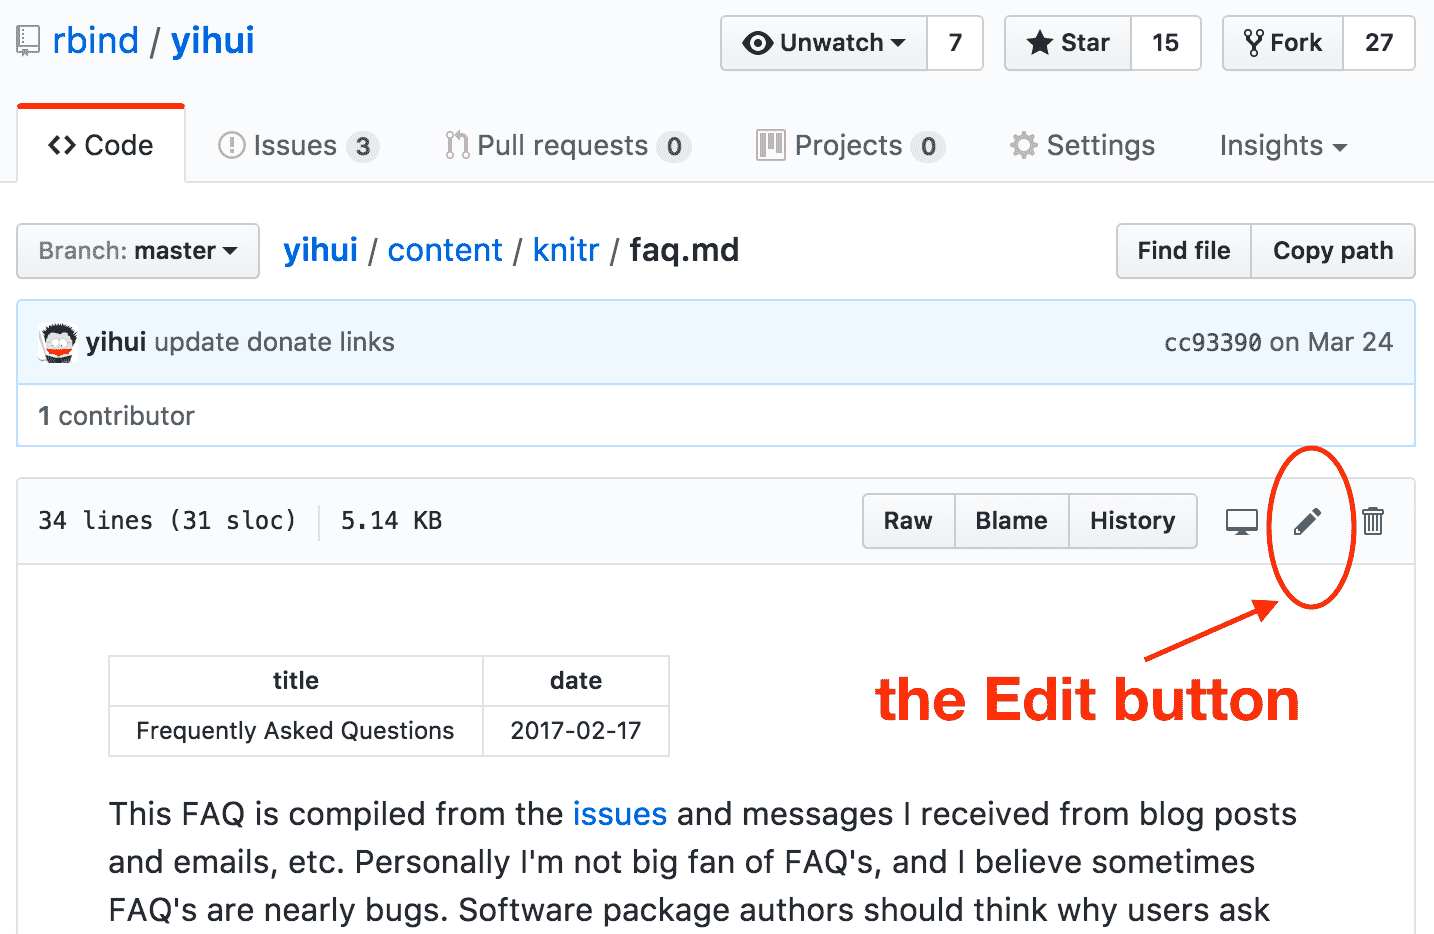
\includegraphics[width=1\linewidth]{images/github-edit} 

}

\caption{Editar un archivo de texto en línea en GitHub.}\label{fig:github-edit}
\end{figure}

Después de digerir el tema XMin y las implementaciones de funciones
adicionales, debería ser mucho más fácil entender las plantillas de
otras personas. Hay una gran cantidad de temas de Hugo, pero las
principales diferencias entre ellos suelen ser estilos. Los componentes
básicos de las plantillas son a menudo similares.

\hypertarget{layouts-personalizados}{%
\section{Layouts personalizados}\label{layouts-personalizados}}

Es muy probable que desee personalizar un tema a menos que lo haya
diseñado. La forma más directa es simplemente hacer cambios directamente
en el tema,\footnote{Si es nuevo en el desarrollo web, tenga cuidado de
  cambiar el contenido dentro del tema. Pequeños cambios como colores y
  tamaños de fuente se pueden encontrar dentro de los archivos CSS del
  tema y pueden modificarse simplemente con el mínimo riesgo de romper
  la funcionalidad del tema.} Pero el problema es que un tema de Hugo
puede ser actualizado constantemente por su autor original para mejoras
o correcciones de errores. De manera similar a la política ``la rompes,
la compras'' (la
\href{https://en.wikipedia.org/wiki/Pottery_Barn_rule}{regla de Pottery
Barn}), una vez que toca el código fuente de otra persona, será
responsable de su mantenimiento futuro, y el autor original no debería
ser responsable de los cambios que haya realizado de su lado. Eso
significa que puede no ser fácil extraer actualizaciones futuras de este
tema a su sitio web (debe leer cuidadosamente los cambios y asegurarse
de que no entren en conflicto con sus cambios), pero si está
completamente satisfecho con el estado actual del tema y no quiere
actualizaciones futuras, está bien modificar los archivos de tema
directamente.

Un autor de tema que tenga en cuenta el hecho de que los usuarios pueden
personalizar su tema generalmente proporcionará dos maneras: una es
proporcionar opciones en \texttt{config.toml}, para que pueda cambiar
estas opciones sin tocar los archivos de la plantilla; la otra es dejar
unos pocos archivos de plantilla livianos en `layouts/' en el tema, para
que pueda anularlos sin tocar los archivos de la plantilla principal.
Tome el tema XMin por ejemplo:

Tengo dos archivos HTML vacíos \texttt{head\_custom.html} y
\texttt{foot\_custom.html} en \texttt{layouts/partials/} en el tema. El
primero se agregará dentro de
\texttt{\textless{}head\textgreater{}\ \textless{}/head\textgreater{}}
de una página, por ejemplo, puede cargar librerías de JavaScript o
incluir hojas de estilo CSS mediante
\texttt{\textless{}link\textgreater{}}. Este último se agregará antes
del pie de página de una página, por ejemplo, puede cargar librerías de
JavaScript adicionales o incrustar comentarios de Disqus allí.

La forma en que personaliza estos dos archivos no es para editarlos
directamente en la carpeta de temas, sino para crear un directorio
\texttt{layouts/partials/} en el directorio raíz de su sitio web, por
ejemplo, su estructura de directorios puede verse así:

\begin{Shaded}
\begin{Highlighting}[]
\ExtensionTok{your-website/}
\NormalTok{├── }\ExtensionTok{config.toml}
\NormalTok{├── }\ExtensionTok{...}
\NormalTok{├── }\ExtensionTok{themes/}
\NormalTok{│   └── }\ExtensionTok{hugo-xmin/}
\NormalTok{│       ├── }\ExtensionTok{...}
\NormalTok{│       └── }\ExtensionTok{layouts/}
\NormalTok{│           ├── }\ExtensionTok{...}
\NormalTok{│           └── }\ExtensionTok{partials}
\NormalTok{│               ├── }\ExtensionTok{foot_custom.html}
\NormalTok{│               ├── }\ExtensionTok{footer.html}
\NormalTok{│               ├── }\ExtensionTok{head_custom.html}
\NormalTok{│               └── }\ExtensionTok{header.html}
\NormalTok{└── }\ExtensionTok{layouts}
\NormalTok{    └── }\ExtensionTok{partials}
\NormalTok{        ├── }\ExtensionTok{foot_custom.html}
\NormalTok{        └── }\ExtensionTok{head_custom.html}
\end{Highlighting}
\end{Shaded}

Todos los archivos en \texttt{layouts/} en el directorio raíz anularán
los archivos con las mismas rutas relativas en
\texttt{themes/hugo-xmin/layouts/}, por ejemplo, el archivo
\texttt{layouts/partials/foot\_custom.html}, cuando se proporcione,
anulará \texttt{themes/hugo-xmin/layouts/partials/foot\_custom.html}.
Eso significa que solo necesita crear y mantener como máximo dos
archivos en \texttt{layouts/} en lugar de mantener todos los archivos
bajo \texttt{themes/}. Tenga en cuenta que este mecanismo de anulación
se aplica a todos los archivos en \texttt{layouts/}, y no está limitado
al directorio \texttt{parials/}. También se aplica a cualquier tema de
Hugo que utilice realmente para su sitio web, y no se limita a
\texttt{hugo-xmin}.

\hypertarget{archivos-estaticos}{%
\section{Archivos estáticos}\label{archivos-estaticos}}

Todos los archivos bajo el directorio
\texttt{static/}\index{Directorio Static} se copian a \texttt{public/}
cuando Hugo procesa un sitio web. Este directorio se usa a menudo para
almacenar archivos web estáticos como imágenes, CSS y archivos de
JavaScript. Por ejemplo, una imagen \texttt{static/foo/bar.png} se puede
incrustar en su publicación usando la sintaxis Markdown
\texttt{!{[}{]}(/foo/bar.png)}.\footnote{El enlace de la imagen depende
  de su configuración \texttt{baseurl} en \texttt{config.toml}. Si no
  contiene un subtrayecto, \texttt{/foo/bar.png} será el enlace de la
  imagen; de lo contrario, tendrá que ajustarlo, por ejemplo, para
  \texttt{baseurl\ =\ "http://example.com/subpath/"}, el enlace a la
  imagen debe ser \texttt{/subpath/foo/bar.png}.}

Por lo general, un tema tiene una carpeta \texttt{static/}, y puede
anular parcialmente sus archivos utilizando el mismo mecanismo que
reemplaza a los \texttt{layouts/} archivos, es decir,
\texttt{static/file} anulará \texttt{themes/theme-name/static/file} . En
el tema XMin, tengo dos archivos CSS \texttt{style.css} y
\texttt{fonts.css}. El primero es la hoja de estilo principal, y el
último es un archivo bastante pequeño para definir tipos de letra
solamente. Es posible que desee definir sus propios tipos de letra, y
solo puede proporcionar un \texttt{static/css/fonts.css} para anular el
del tema, por ejemplo,

\begin{Shaded}
\begin{Highlighting}[]
\NormalTok{body \{}
  \KeywordTok{font-family}\NormalTok{: }\StringTok{"Comic Sans MS"}\NormalTok{, }\DecValTok{cursive}\NormalTok{, }\DecValTok{sans-serif}\NormalTok{;}
\NormalTok{\}}
\NormalTok{code \{}
  \KeywordTok{font-family}\NormalTok{: }\StringTok{"Courier New"}\NormalTok{, Courier, }\DecValTok{monospace}\NormalTok{;}
\NormalTok{\}}
\end{Highlighting}
\end{Shaded}

Para los usuarios de R Markdown, otra aplicación importante del
directorio \texttt{static/} es construir documentos Rmd con formatos de
salida personalizados, es decir, documentos Rmd que no utilizan el
formato \texttt{blogdown::html\_page()} (ver sección
\ref{formatos-de-salida}). Por ejemplo, puede generar un PDF o
presentaciones de documentos Rmd en este directorio, para que Hugo no
los postprocesa, sino que simplemente los copie en \texttt{public/} para
su publicación. Para compilar estos archivos Rmd, debe proporcionar un
script de compilación personalizado \texttt{R/build.R} (consulte la
sección \ref{métodos}). Puede escribir una sola línea de código en este
script\index{blogdown::build\_dir()}:

\begin{Shaded}
\begin{Highlighting}[]
\NormalTok{blogdown}\OperatorTok{::}\KeywordTok{build_dir}\NormalTok{(}\StringTok{"static"}\NormalTok{)}
\end{Highlighting}
\end{Shaded}

La función \texttt{build\_dir()} busca todos los archivos Rmd bajo un
directorio y llama a \texttt{rmarkdown::render()} para compilarlos en
los formatos de salida especificados en los metadatos YAML de los
archivos Rmd. Si sus archivos Rmd no se deben presentar con una simple
llamada \texttt{rmarkdown::render()}, puede proporcionar su propio
código para presentarlos en \texttt{R/build.R}. Hay un mecanismo de
caché integrado en la función \texttt{dir\_desarrollo()}: un archivo Rmd
no se compilará si es anterior a su archivo(s) de salida. Si no desea
este comportamiento, puede obligar a todos los archivos Rmd a volver a
compilarse cada vez: \texttt{build\_dir(force\ =\ TRUE)}.

He proporcionado un ejemplo mínimo en el repositorio de GitHub
\href{https://github.com/yihui/blogdown-static}{yihui/blogdown-static,}
donde puede encontrar dos ejemplos de Rmd en el directorio
\texttt{static/}. Una es una presentación HTML5 basada en el paquete
\textbf{xaringan}, y la otra es un documento PDF basado en
\textbf{bookdown}.

Debe tener precaución con los archivos arbitrarios en \texttt{static/},
debido al mecanismo predominante de Hugo. Es decir, todo en
\texttt{static/} se copiará en \texttt{public/}. Debe asegurarse de que
los archivos que procesa en \texttt{static/} no entrarán en conflicto
con los archivos generados automáticamente por Hugo a partir de
\texttt{content/}. Por ejemplo, si tiene un archivo fuente
\texttt{content/about.md} y un archivo Rmd
\texttt{static/about/index.Rmd} al mismo tiempo, el resultado HTML de
este último sobrescribirá el anterior (tanto Hugo como usted generarán
un archivo de salida con el mismo nombre
\texttt{public/about/index.html}).

\hypertarget{implementacion}{%
\chapter{Implementación}\label{implementacion}}

Dado que el sitio web es básicamente una carpeta que contiene archivos
estáticos, es mucho más fácil de implementar que los sitios web que
requieren lenguajes dinámicos en el servidor, como PHP o bases de datos.
Todo lo que necesita es subir los archivos a un servidor, y generalmente
su sitio web estará en funcionamiento en breve. La pregunta clave es qué
servidor web quiere usar. Si no tiene su propio servidor, puede probar
los que figuran en este capítulo. La mayoría de ellos son gratuitos
(excepto Amazon S3), o al menos ofrecen planes gratuitos. Descargo de
responsabilidad: los autores de este libro no están afiliados a ninguno
de estos servicios o compañías, y no hay garantía de que estos servicios
se presten para siempre.\footnote{Puede encontrar fácilmente otros
  servicios similares si usa su motor de búsqueda}.

Teniendo en cuenta el costo y la amabilidad de los principiantes,
actualmente recomendamos Netlify (\url{https://www.netlify.com}).
Proporciona un plan gratuito que en realidad tiene muchas funciones
útiles. Si no tiene experiencia en publicar sitios web antes, solo
inicie sesión con su cuenta GitHub u otras cuentas, arrastre la carpeta
\texttt{public/} creada por \textbf{blogdown} para su sitio web a la
página de Netlify, y su sitio web estará en línea en unos segundos con
un nombre de subdominio aleatorio del formulario
\texttt{random-word-12345.netlify.com} proporcionado por Netlify (puede
personalizar el nombre). Puede automatizar fácilmente este proceso
(consulte la sección \ref{netlify} para obtener más información). Ya no
necesita luchar con \texttt{ssh} o \texttt{rsync-zrvce}, si sabe lo que
significan estos comandos.

La segunda solución más fácil puede ser Updog (\url{https://updog.co}),
que cuenta con la integración de Dropbox. Publicar un sitio web puede
ser tan fácil como copiar los archivos en la carpeta \texttt{public/} de
su sitio web \textbf{blogdown} en una carpeta de Dropbox. El plan
gratuito de Updog solo ofrece funciones limitadas, y su plan de pago le
dará acceso a funciones mucho más ricas.

Si no le importa utilizar herramientas de línea de comandos o está
familiarizado con GIT/GitHub, puede considerar servicios como GitHub
Pages, Travis CI o Amazon S3 para construir o alojar sus sitios web. No
importa qué servicio use, tenga en cuenta que ninguno de ellos realmente
puede encerrarlo y siempre puede cambiar el servicio. Como mencionamos
anteriormente, una gran ventaja de \textbf{blogdown} es que su sitio web
será una carpeta de archivos estáticos que puede mover a cualquier
servidor web.

\hypertarget{netlify}{%
\section{Netlify}\label{netlify}}

Como acabamos de mencionar, Netlify\index{Netlify} le permite publicar
rápidamente un sitio web cargando la carpeta \texttt{public/} a través
de su interfaz web, y se le asignará un subdominio aleatorio
\texttt{*.netlify.com}.\footnote{Usted no tiene que mantener el dominio
  \texttt{*.netlify.com}. Consulte el apéndice @ref(nombre de dominio)
  para obtener más información.} Este enfoque es bueno para los sitios
web que no se actualizan con frecuencia (o no se actualizan). Sin
embargo, es poco probable que no necesite actualizar su sitio web, por
lo que presentamos un mejor enfoque en esta sección,\footnote{Tenga en
  cuenta que el propósito de esta sección es describir los pasos básicos
  de la publicación de un sitio web con Netlify, y los detalles técnicos
  pueden cambiar de vez en cuando, por lo que la documentación oficial
  de Netlify debería ser la fuente más confiable si tiene alguna
  pregunta o si alguna de las cosas que presentamos aquí no funciona}.
Le llevará unos minutos más completar las configuraciones. Una vez que
está configurado correctamente, todo lo que necesita hacer en el futuro
es actualizar el repositorio fuente, y Netlify llamará a Hugo para que
haga su sitio web automáticamente.

Básicamente, debe alojar todos los archivos fuente de su sitio web en un
repositorio GIT.\footnote{Si el contenido de su sitio \texttt{blogdown}
  no está en el directorio raíz de su repositorio GIT, Netlify no se
  compilará.} No necesita poner el directorio \texttt{public/} bajo
control de versión\footnote{Puede agregar \texttt{public} a
  \texttt{.gitignore} para ignorarlo en GIT.} porque se generará
automáticamente. Actualmente, Netlify admite repositorios GIT alojados
en GitHub, GitLab y BitBucket. Con cualquiera de estas cuentas, puede
iniciar sesión en Netlify desde su página de inicio y seguir la guía
para crear un nuevo sitio desde su repositorio de GIT.

Netlify es compatible con varios generadores de sitios web estáticos,
incluidos Jekyll y Hugo. Para un nuevo sitio, debe especificar un
comando para construir su sitio web, así como también la ruta del
directorio de publicación. Netlify también admite múltiples versiones de
Hugo, por lo que el comando de compilación puede ser el \texttt{hugo}
predeterminado. La versión predeterminada es 0.17, que es demasiado
antigua. Le recomendamos que utilice al menos la versión 0.20. Para
especificar una versión de Hugo mayor o igual a 0.20, debe crear una
variable de entorno \texttt{HUGO\_VERSION} en Netlify. Consulte la
\href{https://www.netlify.com/docs/continuous-deployment/}{documentación
de Netlify} para obtener más información. El directorio de publicación
debe ser \texttt{public} a menos que lo haya cambiado en su
\texttt{config.toml}. La figura @ref(fig: configuración-netlify) muestra
la configuración del sitio web \url{https://t.yihui.name}. No tiene que
seguir la configuración exacta para su propio sitio web; en particular,
es posible que necesite cambiar el valor de la variable de entorno
\texttt{HUGO\_VERSION} a una versión reciente de Hugo.\footnote{Para el
  momento en que se publique este libro, la versión 0.24.1 puede ser
  demasiado antigua.}

\begin{figure}

{\centering 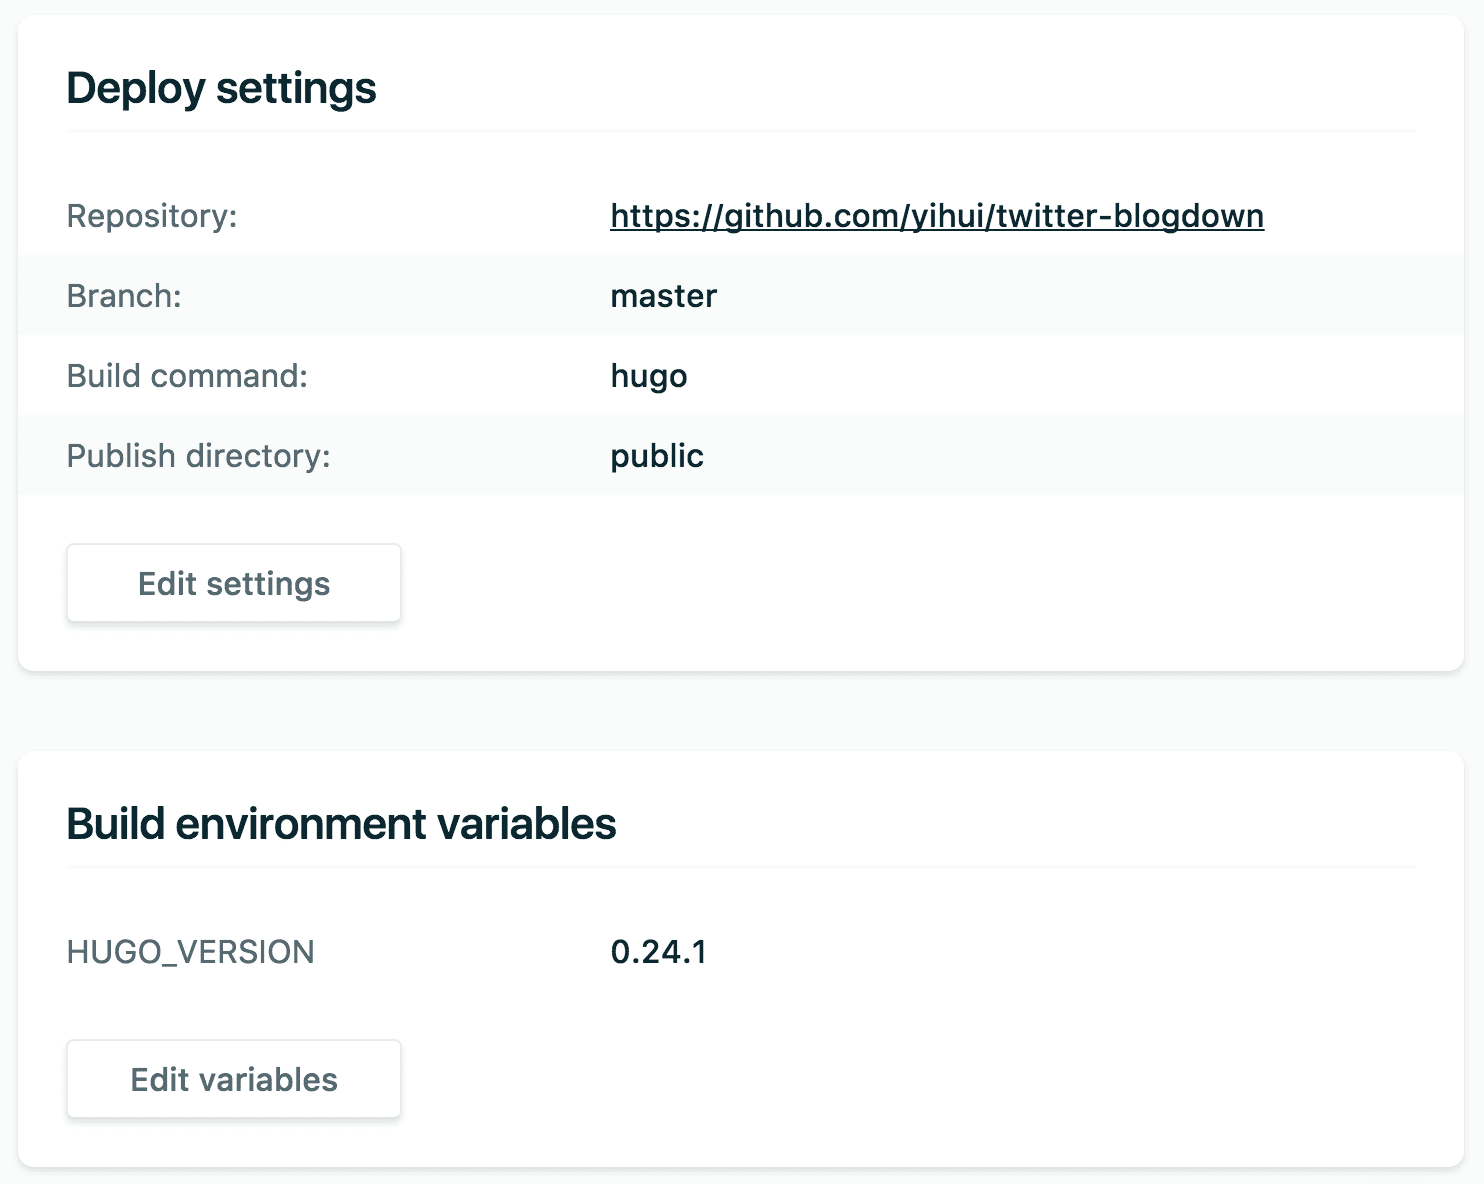
\includegraphics[width=1\linewidth]{images/netlify-settings} 

}

\caption{Configuraciones de ejemplo de un sitio web presentado en Netlify.}\label{fig:netlify-settings}
\end{figure}

Puede tardar uno o dos minutos en implementar su sitio web en Netlify
por primera vez, pero puede ser mucho más rápido más adelante (unos
segundos) cuando actualice el origen de su sitio web, porque Netlify
implementa cambios incrementales en el directorio \texttt{public/}, es
decir, solo se despliegan los archivos más nuevos en comparación con la
última vez.

Después de que su repositorio de GIT esté conectado con Netlify, el
último problema que puede querer resolver es el nombre de
dominio\index{nombre de dominio}, a menos que esté satisfecho con el
subdominio gratuito de Netlify. Si desea utilizar un dominio diferente,
debe configurar algunos registros DNS del dominio para dirigirlo al
servidor de Netlify. Consulte el apéndice @ref(nombre de dominio) para
obtener información general sobre los nombres de dominio.

Si no está familiarizado con los nombres de dominio o no quiere aprender
más sobre ellos, debe tener en cuenta un subdominio gratuito
\texttt{*\ .rbind.io} ofrecido por RStudio, Inc.~Visite el sitio web de
soporte de Rbind \url{https://support.rbind.io} para aprender cómo
solicitar un subdominio. De hecho, la organización Rbind también ofrece
ayuda gratuita sobre cómo configurar un sitio web basado en
\textbf{blogdown}, gracias a una gran cantidad de voluntarios de la
comunidad de R y de estadística.

Netlify es la única solución en este capítulo que no requiere
preinstalar su sitio web. Solo necesita actualizar los archivos fuente,
enviarlos a GitHub y Netlify creará el sitio web para usted.\footnote{Esto
  se denomina ``implementación continua''}. El resto de las soluciones
de este capítulo requerirán que cree su sitio web localmente. y cargue
la carpeta \texttt{public/} explícita o implícitamente. Dicho esto,
ciertamente puede preconstruir su sitio web utilizando cualquier
herramienta, enviarlo a GitHub, y aún así Netlify lo implementará para
usted. Lo que debe hacer es dejar el comando de compilación en blanco y
decirle a Netlify su directorio de publicación (por ejemplo,
\texttt{public/} por defecto de Hugo, pero si su sitio web preconstruido
está bajo el directorio raíz, especifique \texttt{.} como el directorio
de publicación). Entonces Netlify simplemente carga todos los archivos
de este directorio a sus servidores sin reconstruir su sitio web.

\hypertarget{updog}{%
\section{Updog}\label{updog}}

Updog (\url{https://updog.co}) proporciona\index{Updog} un servicio
simple: convierte una carpeta de Dropbox (o Google Drive) especificada
en un sitio web. La idea es que le conceda a Updog el permiso para leer
la carpeta, y actuará como intermediario para mostrar sus archivos en
esta carpeta a sus visitantes. Se debe acceder a esta carpeta a través
de un nombre de dominio, y Updog ofrece un subdominio gratuito
\texttt{*.updog.co}. Por ejemplo, si ha asignado el dominio
\texttt{example.updog.co} a su carpeta de Dropbox, y un visitante desea
ver la página \texttt{https://example.updog.co/foo/index.html}, Updog
leerá el archivo \texttt{foo/index.html} en su carpeta de Dropbox y lo
mostrará al visitante.

Por el momento, el plan gratuito de Updog solo permite un sitio web por
cuenta e insertará un pie de página ``Hosted on Updog'' en sus páginas
web. Puede que no le gusten estas limitaciones. La principal ventaja de
usar Updog es que la publicación de un sitio web se vuelve implícita, ya
que Dropbox sincronizará archivos continuamente. Todo lo que necesita
hacer es asegurarse de que su sitio web se genere en la carpeta correcta
de Dropbox. Esto se puede lograr fácilmente estableciendo la opción
\texttt{publishDir} en \texttt{config.toml}. Por ejemplo, supongamos que
la carpeta que asigna a Updog es
\texttt{\textasciitilde{}/Dropbox/Apps/updog/my-website/}, y su carpeta
fuente está en \texttt{\textasciitilde{}/Dropbox/Apps/updog/my-source/},
entonces puede establecer \texttt{publishDir:\ "../my-website"} en
\texttt{\textasciitilde{}/Dropbox/Apps/updog/my-source/config.toml}.

También puede usar su nombre de dominio personalizado si no desea el
subdominio Updog predeterminado, y solo necesita apuntar el registro
CNAME de su nombre de dominio al subdominio Updog.\footnote{Vea el
  apéndice @ref(nombre de dominio) para obtener más información.}

\hypertarget{github-pages}{%
\section{GitHub Pages}\label{github-pages}}

GitHub Pages (\url{https://pages.github.com}) \index{GitHub Pages} es
una forma muy popular de alojar sitios web estáticos (especialmente los
creados con Jekyll), pero sus ventajas no son obvias ni atractivas en
comparación con Netlify. Le recomendamos que considere Netlify + Hugo
debido a estas razones:

\begin{itemize}
\item
  Actualmente, GitHub Pages no es compatible con HTTPS para nombres de
  dominio personalizados. HTTPS solo funciona para los subdominios
  \texttt{*.github.io}. Esta limitación no existe en Netlify. Puede leer
  el artículo \href{https://https.cio.gov/everything/}{``¿Por qué HTTPS
  para todo?''} para comprender por qué es importante y se le anima a
  activar HTTPS para su sitio web siempre que sea posible.
\item
  Redirigir URLs es incómodo con GitHub Pages pero mucho más sencillo
  con Netlify.\footnote{GitHub Pages utiliza un plugin Jekyll para
    escribir una metaetiqueta \texttt{HTTP-REFRESH} para redirigir
    páginas, y Netlify puede hacer redirecciones 301 o 302 basadas en
    patrones, que puede notificar a los motores de búsqueda que ciertas
    páginas se han movido (de forma permanente o temporal).} Esto es
  importante especialmente cuando tiene un sitio web antiguo que desea
  migrar a Hugo; algunos enlaces pueden estar rotos, en cuyo caso puede
  redireccionarlos fácilmente con Netlify.
\item
  Una de las mejores características de Netlify que no está disponible
  en GitHub Pages es que Netlify puede generar un sitio web único para
  la vista previa cuando se envía un pull request de GitHub a su
  repositorio de GitHub. Esto es extremadamente útil cuando otra persona
  (o incluso usted mismo) propone cambios en su sitio web, ya que tiene
  la oportunidad de ver cómo se vería el sitio web antes de fusionar el
  pull request.
\end{itemize}

Básicamente, Netlify puede hacer todo lo que GitHub Pages puede, pero
todavía hay una pequeña característica que falta, que está estrechamente
vinculada a GitHub, que es GitHub
\href{https://help.github.com/articles/user-organization-and-project-pages/}{Project
Pages.}. Esta función le permite tener sitios web de proyectos en
repositorios separados, por ejemplo, puede tener dos sitios web
independientes \texttt{https://username.github.io/proj-a/} y
\texttt{https://username.github.io/proj-b/}, que corresponde a los
repositorios de GitHub \texttt{username/proj-a} y
\texttt{username/proj-b}, respectivamente. Sin embargo, dado que puede
conectar cualquier repositorio de GitHub con Netlify, y cada repositorio
puede asociarse con un nombre de dominio o subdominio, puede reemplazar
las páginas de proyecto de GitHub con diferentes subdominios como
\texttt{proj-a.netlify.com} y \texttt{proj-b.netlify.com}. La limitación
real es que no puede usar subcampos en la URL pero puede usar cualquier
(sub)nombre de dominio.

Aunque GitHub no es compatible oficialmente con Hugo (solo es compatible
con Jekyll), puede publicar cualquier archivo HTML estático en GitHub
Pages, incluso si no están compiladas con Jekyll. El primer requisito
para usar GitHub Pages es que debe crear un repositorio de GitHub
llamado \texttt{username.github.io} debajo de su cuenta (reemplace
\texttt{username} con su nombre de usuario GitHub real), y lo que queda
es llevar los archivos de su sitio web a este repositorio. La
documentación completa de GitHub Pages está en
\url{https://pages.github.com}, y por favor ignore todo lo relacionado
con Jekyll a menos que realmente use Jekyll en lugar de Hugo. Para
asegurarse de que GitHub no reconstruya su sitio web utilizando Jekyll y
simplemente publique los archivos que envía al repositorio, debe crear
un archivo (oculto) llamado \texttt{.nojekyll} en el
repositorio.\footnote{Puede usar la función en R
  \texttt{file.create(\textquotesingle{}.nojekyll\textquotesingle{})}
  para crear este archivo si no sabe cómo hacerlo.} GitHub ofrece un
subdominio gratuito \texttt{username.github.io}, y puede usar su propio
nombre de dominio configurando sus registros A o CNAME para apuntarlo a
GitHub Pages (consulte la documentación de GitHub Pages para obtener
instrucciones).

Su directorio \texttt{public/} debe ser el repositorio de GIT. Tienes
dos opciones posibles para configurar este repositorio localmente. La
primera opción es seguir la estructura predeterminada de un sitio web de
Hugo como el siguiente diagrama e inicializar el repositorio de GIT bajo
el directorio \texttt{public/}:

\begin{Shaded}
\begin{Highlighting}[]
\ExtensionTok{source/}
\NormalTok{│}
\NormalTok{├── }\ExtensionTok{config.toml}
\NormalTok{├── }\ExtensionTok{content/}
\NormalTok{├── }\ExtensionTok{themes/}
\NormalTok{├── }\ExtensionTok{...}
\NormalTok{└── }\ExtensionTok{public/}
    \KeywordTok{|}
\NormalTok{    ├── }\ExtensionTok{.git/}
\NormalTok{    ├── }\ExtensionTok{.nojekyll}
\NormalTok{    ├── }\ExtensionTok{index.html}
\NormalTok{    ├── }\ExtensionTok{about/}
\NormalTok{    └── }\ExtensionTok{...}
\end{Highlighting}
\end{Shaded}

Si sabe cómo usar la línea de comandos, cambie el directorio de trabajo
a \texttt{public/}, e inicialice el repositorio de GIT allí:

\begin{Shaded}
\begin{Highlighting}[]
\BuiltInTok{cd}\NormalTok{ public}
\FunctionTok{git}\NormalTok{ init}
\FunctionTok{git}\NormalTok{ remote add origin https://github.com/username/username.github.io}
\end{Highlighting}
\end{Shaded}

La otra opción es clonar el repositorio de GitHub que creó en el mismo
directorio que el origen de su sitio web:

\begin{Shaded}
\begin{Highlighting}[]
\FunctionTok{git}\NormalTok{ clone https://github.com/username/username.github.io}
\end{Highlighting}
\end{Shaded}

Y la estructura debería lucir más o menos así:

\begin{Shaded}
\begin{Highlighting}[]
\ExtensionTok{source/}
\NormalTok{│}
\NormalTok{├── }\ExtensionTok{config.toml}
\NormalTok{├── }\ExtensionTok{content/}
\NormalTok{├── }\ExtensionTok{themes/}
\NormalTok{└── }\ExtensionTok{...}

\ExtensionTok{username.github.io/}
\NormalTok{│}
\NormalTok{├── }\ExtensionTok{.git/}
\NormalTok{├── }\ExtensionTok{.nojekyll}
\NormalTok{├── }\ExtensionTok{index.html}
\NormalTok{├── }\ExtensionTok{about/}
\NormalTok{└── }\ExtensionTok{...}
\end{Highlighting}
\end{Shaded}

El directorio de origen y el directorio \texttt{username.github.io}
están bajo el mismo directorio principal. En este caso, debe establecer
la opción \texttt{publishDir:\ "../username.github.io"} en
\texttt{source/config.toml}.

\hypertarget{travis-github}{%
\section{Travis + GitHub}\label{travis-github}}

Si\index{Travis CI} decide no seguir nuestra recomendación de usar
Netlify para implementar su sitio web, debemos advertirle que el enfoque
de esta sección requerirá un conocimiento sustancial sobre GIT, GitHub,
Travis CI (\url{https://travis-ci.org}), y la línea de comandos de
Linux, que dejaremos que aprenda por su cuenta. La principal ventaja de
publicar a través de Travis CI es que puede compilar todas sus
publicaciones de Rmd en Travis CI (en la nube) en lugar de su
computadora local.

En caso de que no esté familiarizado con Travis, este es un servicio de
verificación continua de su software en una máquina virtual cada vez que
haga push a cambios en GitHub. Es principalmente para probar software,
pero dado que puede ejecutar muchos comandos en su máquina virtual,
puede usar la máquina virtual para hacer otras cosas, por ejemplo,
instalar R y el paquete \textbf{blogdown} para crear sitios web. Antes
de mostrarle cómo, me gustaría mencionar dos cuestiones que debe tener
en cuenta:

\begin{itemize}
\item
  Personalmente, prefiero echar un vistazo a la salida en GIT para ver
  los cambios cuando tengo cualquier salida que se calcula dinámicamente
  desde R, para que sepa con certeza qué voy a publicar exactamente. Con
  Travis, es algo impredecible porque es completamente automático y no
  tiene la oportunidad de ver el nuevo contenido o los resultados que se
  publicarán. Hay muchos factores que pueden afectar la construcción del
  sitio: la versión de R, la disponibilidad de ciertos paquetes en R,
  las dependencias del sistema y la conexión de red, etc.
\item
  El tiempo requerido para compilar todos los archivos Rmd puede ser muy
  largo y causar tiempos de espera en Travis, dependiendo de cuánto
  tiempo consuma su código en R. Hay un mecanismo de almacenamiento en
  caché en \textbf{blogdown} para acelerar la construcción de su sitio
  (consulte la sección \ref{métodos}), y si usa Travis para construir su
  sitio web, no se beneficiará de este mecanismo de almacenamiento en
  caché a menos que aproveche el almacenamiento en caché de Travis.
  Tiene que almacenar en caché los directorios \texttt{content/},
  \texttt{static/}, y \texttt{blogdown/}, pero el caché de Travis es un
  poco frágil, en mi experiencia. Algunas veces la memoria caché puede
  ser purgada por razones desconocidas. Además, no puede almacenar en
  caché directamente \texttt{content/} y \texttt{static/}, porque Travis
  clona su repositorio antes de restaurar el caché, lo que significa que
  los archivos viejos del \texttt{content/} y \texttt{static/}
  almacenados en caché pueden sobrescribir los nuevos archivos que usted
  envió a GitHub.
\end{itemize}

El segundo problema se puede resolver, pero no quiero explicar cómo en
este libro, ya que la solución es demasiado complicada. Si realmente
desea usar Travis para construir su sitio web y encontrarse con este
problema, puede presentar un issue en el repositorio de GitHub
\url{https://github.com/yihui/travis-blogdown}. De hecho, este
repositorio es un ejemplo mínimo que creé para mostrar cómo crear un
sitio web en Travis y publicarlo en GitHub Pages.

La documentación de Travis muestra cómo implementar un sitio en GitHub
Pages: \url{https://docs.travis-ci.com/user/deployment/pages/}, pero no
muestra cómo crear un sitio. Aquí está el archivo de configuración de
Travis, \texttt{.travis.yml}, para el repositorio
\texttt{travis-blogdown}:

\begin{Shaded}
\begin{Highlighting}[]
\FunctionTok{language:}\AttributeTok{ r}
\FunctionTok{dist:}\AttributeTok{ trusty}
\FunctionTok{sudo:}\AttributeTok{ false}

\FunctionTok{branches:}
  \FunctionTok{only:}
    \KeywordTok{-}\NormalTok{ master}

\FunctionTok{cache:}
  \FunctionTok{packages:}\AttributeTok{ yes}
  \FunctionTok{directories:}
    \KeywordTok{-}\NormalTok{ $HOME/bin}

\FunctionTok{before_script:}
  \KeywordTok{-} \StringTok{"Rscript -e 'blogdown::install_hugo()'"}

\FunctionTok{script:}
  \KeywordTok{-} \StringTok{"Rscript -e 'blogdown::build_site()'"}

\FunctionTok{deploy:}
  \FunctionTok{provider:}\AttributeTok{ pages}
  \FunctionTok{skip_cleanup:}\AttributeTok{ true}
  \FunctionTok{github_token:}\AttributeTok{ $GITHUB_TOKEN}
  \FunctionTok{on:}
    \FunctionTok{branch:}\AttributeTok{ master}
  \FunctionTok{local_dir:}\AttributeTok{ public}
  \FunctionTok{fqdn:}\AttributeTok{ travis-blogdown.yihui.name}
\end{Highlighting}
\end{Shaded}

La clave es que instalemos Hugo a través de
\texttt{blogdown::install\_hugo()} y construyamos el sitio a través de
\texttt{blogdown::build\_site()}. Para engañar a Travis para que cree
este repositorio como un paquete en R, debe tener un archivo
\texttt{DESCRIPTION} en el repositorio, de lo contrario, su sitio web no
se compilará.

\begin{Shaded}
\begin{Highlighting}[]
\FunctionTok{Package:}\AttributeTok{ placeholder}
\FunctionTok{Type:}\AttributeTok{ Website}
\FunctionTok{Title:}\AttributeTok{ Does not matter.}
\FunctionTok{Version:}\AttributeTok{ 0.0.1}
\FunctionTok{Imports:}\AttributeTok{ blogdown}
\FunctionTok{Remotes:}\AttributeTok{ rstudio/blogdown}
\end{Highlighting}
\end{Shaded}

Hay algunas cosas más que explicar y enfatizar en \texttt{.travis.yml}:

\begin{itemize}
\item
  La opción \texttt{branches} especifica que solo los cambios en la rama
  \texttt{master} activarán la construcción en Travis.
\item
  La opción \texttt{cache} especifica todos los paquetes en R que se
  almacenarán en caché, por lo que la próxima vez será más rápido crear
  el sitio (no es necesario volver a instalar los paquetes en R desde el
  origen). El directorio \texttt{bin/} en el directorio de inicio
  también se almacena en caché porque Hugo está instalado allí, y la
  próxima vez que Hugo no necesite ser reinstalado.
\item
  Para la opción \texttt{deploy}, hay una variable de entorno llamada
  \texttt{GITHUB\_TOKEN}, y he especificado su valor para ser un token
  de acceso personal de GitHub a través de la configuración de Travis de
  este repositorio, para que Travis pueda escribir en mi repositorio
  después de que el sitio web está construido. La opción \texttt{on}
  especifica que la implementación solo ocurrirá cuando se construya la
  rama \texttt{master}. La opción \texttt{local\_dir} es el directorio
  de publicación, que debe ser `público' por defecto en Hugo. Por
  defecto, el sitio web se envía a la rama \texttt{gh-pages} de este
  repositorio. La opción \texttt{fqdn} especifica el dominio
  personalizado del sitio web. He establecido un registro CNAME (ver
  apéndice @ref(nombre de dominio)) para apuntar
  \texttt{travis-blogdown.yihui.name} a \texttt{yihui.github.io}, para
  que GitHub pueda servir a este sitio web a través de este dominio (de
  hecho, Travis escribirá un archivo \texttt{CNAME} que contiene el
  dominio en la rama \texttt{gh-pages}).
\end{itemize}

Si utiliza el repositorio \texttt{username.github.io} en GitHub, el
sitio web debe ser enviado a su rama \texttt{master} en lugar de
\texttt{gh-pages} (esta es la única excepción). Recomiendo que separe el
repositorio fuente y el repositorio de salida. Por ejemplo, puede tener
un repositorio \texttt{website-source} con la misma configuración que el
\texttt{.travis.yml} anterior, excepto dos nuevas opciones bajo
\texttt{deploy}:

\begin{Shaded}
\begin{Highlighting}[]
\FunctionTok{deploy:}
\NormalTok{  ...}
  \FunctionTok{repo:}\AttributeTok{ username/username.github.io}
  \FunctionTok{target_branch:}\AttributeTok{ master}
\end{Highlighting}
\end{Shaded}

Esto significa que el sitio web será enviado a la rama \texttt{master}
del repositorio \texttt{username/username.github.io} (recuerde
reemplazar \texttt{username} con su nombre de usuario real).

También puede implementar su sitio web en Amazon S3\index{Amazon S3}, y
la configuración desde R es muy similar a lo que hemos introducido para
GitHub Pages. La única diferencia está en el último paso, donde cambia
el destino de GitHub Pages a Amazon S3. Para obtener más información,
consulte la documentación de Travis:
\url{https://docs.travis-ci.com/user/deployment/s3/}.

\hypertarget{gitlab-pages}{%
\section{GitLab Pages}\label{gitlab-pages}}

GitLab (\url{http://gitlab.com}) es una forma muy popular de alojar el
código fuente de su proyecto. GitLab tiene un
\href{https://about.gitlab.com/features/gitlab-ci-cd/}{servicio de
Integración y Despliegue Integrado (CI/CD)} que se puede usar para
alojar sitios web estáticos, llamados
\href{https://about.gitlab.com/features/pages/}{Páginas de GitLab}. La
principal ventaja de utilizar GitLab Pages es que podrá compilar todas
sus publicaciones Rmd a través de su servicio CI/CD en lugar de su
computadora local y cualquier contenido generado, como archivos HTML, se
copiará automáticamente en el servidor web. Tenga en cuenta que este
enfoque tiene problemas similares a los del enfoque Travis + GitHub en
la sección \ref{travis-github}.

El servicio CI/CD de GitLab usa las instrucciones almacenadas en el
archivo YAML \texttt{.gitlab-ci.yml} en el repositorio. Aquí hay un
archivo de configuración de muestra \texttt{.gitlab-ci.yml} del
repositorio de ejemplo \url{https://gitlab.com/rgaiacs/blogdown-gitlab}:

\begin{Shaded}
\begin{Highlighting}[]
\FunctionTok{image:}\AttributeTok{ debian:buster-slim}

\FunctionTok{before_script:}
  \KeywordTok{-}\NormalTok{ apt-get update && apt-get -y install pandoc r-base}
  \KeywordTok{-} \FunctionTok{R -e "install.packages('blogdown',repos='http:}\AttributeTok{//cran.rstudio.com')"}
  \KeywordTok{-} \FunctionTok{R -e "blogdown:}\AttributeTok{:install_hugo()"}

\FunctionTok{pages:}
  \FunctionTok{script:}
    \KeywordTok{-} \FunctionTok{R -e "blogdown:}\AttributeTok{:build_site()"}
  \FunctionTok{artifacts:}
    \FunctionTok{paths:}
      \KeywordTok{-}\NormalTok{ public}
  \FunctionTok{only:}
    \KeywordTok{-}\NormalTok{ master}
\end{Highlighting}
\end{Shaded}

La opción \texttt{image} especifica qué imagen de
\href{https://www.docker.com}{Docker} se usará como punto de inicio.
Estamos utilizando una imagen de Debian, pero se puede usar cualquier
imagen de \href{https://hub.docker.com/}{Docker Hub}. Otras
configuraciones y opciones son similares a \texttt{.travis.yml} en la
sección \ref{travis-github}. El ejemplo anterior genera el sitio web en
\url{https://rgaiacs.gitlab.io/blogdown-gitlab}.

\hypertarget{migration}{%
\chapter{Migration}\label{migration}}

Usually, it is easier to start a new website than
migrating\index{Site Migration} an old one to a new framework, but you
may have to do it anyway because of the useful content on the old
website that should not simply be discarded. A lazy solution is to leave
the old website as is, start a new website with a new domain, and
provide a link to the old website. This may be a hassle to your readers,
and they may not be able to easily discover the gems that you created on
your old website, so I recommend that you migrate your old posts and
pages to the new website if possible.

This process may be easy or hard, depending on how complicated your old
website is. The bad news is that there is unlikely to be a universal or
magical solution, but I have provided some helper functions in
\textbf{blogdown} as well as a Shiny application to assist you, which
may make it a little easier for you to migrate from Jekyll and WordPress
sites.

To give you an idea about the possible amount of work required, I can
tell you that it took me a whole week (from the morning to midnight
every day) to migrate several of my personal Jekyll-based websites to
Hugo and \textbf{blogdown}. The complication in my case was not only
Jekyll, but also the fact that I built several separate Jekyll websites
(because I did not have a choice in Jekyll) and I wanted to unite them
in the same repository. Now my two blogs (Chinese and English), the
\textbf{knitr} \citep{R-knitr} package documentation, and the
\textbf{animation} package \citep{R-animation} documentation are
maintained in the same repository: \url{https://github.com/rbind/yihui}.
I have about 1000 pages on this website, most of which are blog posts.
It used to take me more than 30 seconds to preview my blog in Jekyll,
and now it takes less than 2 seconds to build the site in Hugo.

Another complicated example is the website of Rob J Hyndman
(\url{https://robjhyndman.com}). He started his website in 1993 (12
years before me), and had accumulated a lot of content over the years.
You can read the post
\url{https://support.rbind.io/2017/05/15/converting-robjhyndman-to-blogdown/}
for the stories about how he migrated his WordPress website to
\textbf{blogdown}. The key is that you probably need a long
international flight when you want to migrate a complicated website.

A simpler example is the Simply Statistics blog
(\url{https://simplystatistics.org}). Originally it was built on
Jekyll\footnote{It was migrated from WordPress a few years ago. The
  WordPress site was actually migrated from an earlier Tumblr blog.} and
the source was hosted in the GitHub repository
\url{https://github.com/simplystats/simplystats.github.io}. I
volunteered to help them move to \textbf{blogdown}, and it took me about
four hours. My time was mostly spent on cleaning up the YAML metadata of
posts and tweaking the Hugo theme. They had about 1000 posts, which
sounds like a lot, but the number does not really matter, because I
wrote an R script to process all posts automatically. The new repository
is at \url{https://github.com/rbind/simplystats}.

If you do not really have too many pages (e.g., under 20), I recommend
that you cut and paste them to Markdown files, because it may actually
take longer to write a script to process these pages.

It is likely that some links will be broken after the migration because
Hugo renders different links for your pages and posts. In that case, you
may either fix the permanent links (e.g., by tweaking the slug of a
post), or use 301 redirects (e.g., on Netlify).

\hypertarget{from-jekyll}{%
\section{From Jekyll}\label{from-jekyll}}

When converting a Jekyll\index{Jekyll} website to Hugo, the most
challenging part is the theme. If you want to keep exactly the same
theme, you will have to rewrite your Jekyll templates using Hugo's
syntax (see Section \ref{templates}). However, if you can find an
existing theme in Hugo (\url{https://themes.gohugo.io}), things will be
much easier, and you only need to move the content of your website to
Hugo, which is relatively easy. Basically, you copy the Markdown pages
and posts to the \texttt{content/} directory in Hugo and tweak these
text files.

Usually, posts in Jekyll are under the \texttt{\_posts/} directory, and
you can move them to \texttt{content/post/} (you are free to use other
directories). Then you need to define a custom rule for permanent URLs
in \texttt{config.toml} like (see Section \ref{options}):

\begin{Shaded}
\begin{Highlighting}[]
\NormalTok{[permalinks]}
\NormalTok{    post }\OperatorTok{=} \StringTok{"/:year/:month/:day/:slug/"}
\end{Highlighting}
\end{Shaded}

This depends on the format of the URLs you used in Jekyll (see the
\texttt{permalink} option in your \texttt{\_config.yml}).

If there are static assets like images, they can be moved to the
\texttt{static/} directory in Hugo.

Then you need to use your favorite tool with some string manipulation
techniques to process all Markdown files. If you use R, you can list all
Markdown files and process them one by one in a loop. Below is a sketch
of the code:

\begin{Shaded}
\begin{Highlighting}[]
\NormalTok{files =}\StringTok{ }\KeywordTok{list.files}\NormalTok{(}
  \StringTok{'content/'}\NormalTok{, }\StringTok{'[.](md|markdown)$'}\NormalTok{, }\DataTypeTok{full.names =} \OtherTok{TRUE}\NormalTok{,}
  \DataTypeTok{recursive =} \OtherTok{TRUE}
\NormalTok{)}
\ControlFlowTok{for}\NormalTok{ (f }\ControlFlowTok{in}\NormalTok{ files) \{}
\NormalTok{  blogdown}\OperatorTok{:::}\KeywordTok{process_file}\NormalTok{(f, }\ControlFlowTok{function}\NormalTok{(x) \{}
    \CommentTok{# process x here and return the modified x}
\NormalTok{    x}
\NormalTok{  \})}
\NormalTok{\}}
\end{Highlighting}
\end{Shaded}

The \texttt{process\_file()} function is an internal helper function in
\textbf{blogdown}. It takes a filename and a processor function to
manipulate the content of the file, and writes the modified text back to
the file.

To give you an idea of what a processor function may look like, I
provided a few simple helper functions in \textbf{blogdown}, and below
are two of them:

\begin{Shaded}
\begin{Highlighting}[]
\NormalTok{blogdown}\OperatorTok{:::}\NormalTok{remove_extra_empty_lines}
\end{Highlighting}
\end{Shaded}

\begin{verbatim}
function (f) 
process_file(f, function(x) {
    x = paste(gsub("\\s+$", "", x), collapse = "\n")
    trim_ws(gsub("\n{3,}", "\n\n", x))
})
<environment: namespace:blogdown>
\end{verbatim}

\begin{Shaded}
\begin{Highlighting}[]
\NormalTok{blogdown}\OperatorTok{:::}\NormalTok{process_bare_urls}
\end{Highlighting}
\end{Shaded}

\begin{verbatim}
function (f) 
process_file(f, function(x) {
    gsub("\\[([^]]+)]\\(\\1/?\\)", "<\\1>", x)
})
<environment: namespace:blogdown>
\end{verbatim}

The first function substitutes two or more empty lines with a single
empty line. The second function replaces links of the form
\texttt{{[}url{]}(url)} with \texttt{\textless{}url\textgreater{}}.
There is nothing wrong with excessive empty lines or the syntax
\texttt{{[}url{]}(url)}, though. These helper functions may make your
Markdown text a little cleaner. You can find all such helper functions
at \url{https://github.com/rstudio/blogdown/blob/master/R/clean.R}. Note
they are not exported from \textbf{blogdown}, so you need triple colons
to access them.

The YAML metadata of your posts may not be completely clean, especially
when your Jekyll website was actually converted from an earlier
WordPress website. The internal helper function
\texttt{blogdown:::modify\_yaml()} may help you clean up the metadata.
For example, below is the YAML metadata of a blog post of Simply
Statistics when it was built on Jekyll:

\begin{Shaded}
\begin{Highlighting}[]
\OtherTok{---}
\FunctionTok{id:}\AttributeTok{ 4155}
\FunctionTok{title:}\AttributeTok{ Announcing the JHU Data Science Hackathon 2015}
\FunctionTok{date:}\AttributeTok{ 2015-07-28T13:31:04+00:00}
\FunctionTok{author:}\AttributeTok{ Roger Peng}
\FunctionTok{layout:}\AttributeTok{ post}
\FunctionTok{guid:}\AttributeTok{ http://simplystatistics.org/?p=4155}
\FunctionTok{permalink:}\AttributeTok{ /2015/07/28/announcing-the-jhu-data-science-hackathon-2015}
\FunctionTok{pe_theme_meta:}
  \KeywordTok{-} \StringTok{'O:8:"stdClass":2:\{s:7:"gallery";O:8:"stdClass":...\}'}
\FunctionTok{al2fb_facebook_link_id:}
  \KeywordTok{-}\NormalTok{ 136171103105421_837886222933902}
\FunctionTok{al2fb_facebook_link_time:}
  \KeywordTok{-} \FunctionTok{2015-07-28T17:}\AttributeTok{31:11+00:00}
\FunctionTok{al2fb_facebook_link_picture:}
  \KeywordTok{-} \FunctionTok{post=http:}\AttributeTok{//simplystatistics.org/?al2fb_image=1}
\FunctionTok{dsq_thread_id:}
  \KeywordTok{-}\NormalTok{ 3980278933}
\FunctionTok{categories:}
  \KeywordTok{-}\NormalTok{ Uncategorized}
\OtherTok{---}
\end{Highlighting}
\end{Shaded}

You can discard the YAML fields that are not useful in Hugo. For
example, you may only keep the fields \texttt{title}, \texttt{author},
\texttt{date}, \texttt{categories}, and \texttt{tags}, and discard other
fields. Actually, you may also want to add a \texttt{slug} field that
takes the base filename of the post (with the leading date removed). For
example, when the post filename is
\texttt{2015-07-28-announcing-the-jhu-data-science-hackathon-2015.md},
you may want to add
\texttt{slug:\ announcing-the-jhu-data-science-hackathon-2015} to make
sure the URL of the post on the new site remains the same.

Here is the code to process the YAML metadata of all posts:

\begin{Shaded}
\begin{Highlighting}[]
\ControlFlowTok{for}\NormalTok{ (f }\ControlFlowTok{in}\NormalTok{ files) \{}
\NormalTok{  blogdown}\OperatorTok{:::}\KeywordTok{modify_yaml}\NormalTok{(f, }\DataTypeTok{slug =} \ControlFlowTok{function}\NormalTok{(old, yaml) \{}
    \CommentTok{# YYYY-mm-dd-name.md -> name}
    \KeywordTok{gsub}\NormalTok{(}\StringTok{'^}\CharTok{\textbackslash{}\textbackslash{}}\StringTok{d\{4\}-}\CharTok{\textbackslash{}\textbackslash{}}\StringTok{d\{2\}-}\CharTok{\textbackslash{}\textbackslash{}}\StringTok{d\{2\}-|[.](md|markdown)'}\NormalTok{, }\StringTok{''}\NormalTok{, f)}
\NormalTok{  \}, }\DataTypeTok{categories =} \ControlFlowTok{function}\NormalTok{(old, yaml) \{}
    \CommentTok{# remove the Uncategorized category}
    \KeywordTok{setdiff}\NormalTok{(old, }\StringTok{'Uncategorized'}\NormalTok{)}
\NormalTok{  \}, }\DataTypeTok{.keep_fields =} \KeywordTok{c}\NormalTok{(}
    \StringTok{'title'}\NormalTok{, }\StringTok{'author'}\NormalTok{, }\StringTok{'date'}\NormalTok{, }\StringTok{'categories'}\NormalTok{, }\StringTok{'tags'}\NormalTok{, }\StringTok{'slug'}
\NormalTok{  ), }\DataTypeTok{.keep_empty =} \OtherTok{FALSE}\NormalTok{)}
\NormalTok{\}}
\end{Highlighting}
\end{Shaded}

You can pass a file path to \texttt{modify\_yaml()}, define new YAML
values (or functions to return new values based on the old values), and
decide which fields to preserve (\texttt{.keep\_fields}). You may
discard empty fields via \texttt{.keep\_empty\ =\ FALSE}. The processed
YAML metadata is below, which looks much cleaner:

\begin{Shaded}
\begin{Highlighting}[]
\OtherTok{---}
\FunctionTok{title:}\AttributeTok{ Announcing the JHU Data Science Hackathon 2015}
\FunctionTok{author:}\AttributeTok{ Roger Peng}
\FunctionTok{date:}\AttributeTok{ }\StringTok{'2015-07-28T13:31:04+00:00'}
\FunctionTok{slug:}\AttributeTok{ announcing-the-jhu-data-science-hackathon-2015}
\OtherTok{---}
\end{Highlighting}
\end{Shaded}

\hypertarget{from-wordpress}{%
\section{From WordPress}\label{from-wordpress}}

From our experience, the best way to import WordPress\index{WordPress}
blog posts to Hugo is to import them to Jekyll, and write an R script to
clean up the YAML metadata of all pages if necessary, instead of using
the migration tools listed on the
\href{https://gohugo.io/tools/}{official guide,} including the WordPress
plugin \texttt{wordpress-to-hugo-exporter}.

To our knowledge, the best tool to convert a WordPress website to Jekyll
is the Python tool \href{https://github.com/thomasf/exitwp}{Exitwp.} Its
author has provided detailed instructions on how to use it. You have to
know how to install Python libraries and execute Python scripts. If you
do not, I have provided an online tool at
\url{https://github.com/yihui/travis-exitwp}. You can upload your
WordPress XML file there, and get a download link to a ZIP archive that
contains your posts in Markdown.

The biggest challenge in converting WordPress posts to Hugo is to clean
up the post content in Markdown. Fortunately, I have done this for three
different WordPress blogs,\footnote{The RViews blog
  (\url{https://rviews.rstudio.com}), the RStudio blog
  (\url{https://blog.rstudio.com}), and Karl Broman's blog
  (\url{http://kbroman.org}). The RViews blog took me a few days. The
  RStudio blog took me one day. Karl Broman's blog took me an hour.} and
I think I have managed to automate this process as much as possible. You
may refer to the pull request I submitted to Karl Broman to convert his
WordPress posts to Markdown
(\url{https://github.com/kbroman/oldblog_xml/pull/1}), in which I
provided both the R script and the Markdown files. I recommend that you
go to the ``Commits'' tab and view all my GIT commits one by one to see
the full process.

The key is the R script
\url{https://github.com/yihui/oldblog_xml/blob/master/convert.R}, which
converts the WordPress XML file to Markdown posts and cleans them.
Before you run this script on your XML file, you have to adjust a few
parameters, such as the XML filename, your old WordPress site's URL, and
your new blog's URL.

Note that this script depends on the Exitwp tool. If you do not know how
to run Exitwp, please use the online tool I mentioned before
(travis-exitwp), and skip the R code that calls Exitwp.

The Markdown posts should be fairly clean after the conversion, but
there may be remaining HTML tags in your posts, such as
\texttt{\textless{}table\textgreater{}} and
\texttt{\textless{}blockquote\textgreater{}}. You will need to manually
clean them, if any exist.

\hypertarget{from-other-systems}{%
\section{From other systems}\label{from-other-systems}}

If you have a website built by other applications or systems, your best
way to go may be to import your website to WordPress first, export it to
Jekyll, and clean up the Markdown files. You can try to search for
solutions like ``how to import blogger.com to WordPress'' or ``how to
import Tumblr to WordPress.''

If you are very familiar with web scraping techniques, you can also
scrape the HTML pages of your website, and convert them to Markdown via
Pandoc, e.g.,

\begin{Shaded}
\begin{Highlighting}[]
\NormalTok{rmarkdown}\OperatorTok{::}\KeywordTok{pandoc_convert}\NormalTok{(}
  \StringTok{'foo.html'}\NormalTok{, }\DataTypeTok{to =} \StringTok{'markdown'}\NormalTok{, }\DataTypeTok{output =} \StringTok{'foo.md'}
\NormalTok{)}
\end{Highlighting}
\end{Shaded}

I have actually tried this way on a website, but was not satisfied,
since I still had to heavily clean up the Markdown files. If your
website is simpler, this approach may work better for you.

\hypertarget{other-generators}{%
\chapter{Other Generators}\label{other-generators}}

We mentioned the possibility to bypass Hugo and use your own building
method in Section \ref{methods}. Basically you have to build the site
using \texttt{blogdown::build\_site(method\ =\ "custom")}, and provide
your own building script \texttt{/R/build.R}. In this chapter, we show
you how to work with other popular static site generators like Jekyll
and Hexo. Besides these static site generators written in other
languages, there is actually a simple site generator written in R
provided in the \textbf{rmarkdown} package \citep{R-rmarkdown}, and we
will introduce it in Section \ref{rmd-website}.

\hypertarget{jekyll}{%
\section{Jekyll}\label{jekyll}}

For Jekyll (\url{https://jekyllrb.com}) \index{Jekyll}users, I have
prepared a minimal example in the GitHub repository
\href{https://github.com/yihui/blogdown-jekyll}{yihui/blogdown-jekyll.}
If you clone or download this repository and open
\texttt{blogdown-jekyll.Rproj} in RStudio, you can still use all addins
mentioned in Section \ref{rstudio-ide}, such as ``New Post,'' ``Serve
Site,'' and ``Update Metadata,'' but it is Jekyll instead of Hugo that
builds the website behind the scenes now.

I assume you are familiar with Jekyll, and I'm not going to introduce
the basics of Jekyll in this section. For example, you should know what
the \texttt{\_posts/} and \texttt{\_site/} directories mean.

The key pieces of this \textbf{blogdown-jekyll} project are the files
\texttt{.Rprofile}, \texttt{R/build.R}, and \texttt{R/build\_one.R}. I
have set some global R options for this project in
\texttt{.Rprofile}:\footnote{If you are not familiar with this file,
  please read Section \ref{global-options}.}

\begin{Shaded}
\begin{Highlighting}[]
\KeywordTok{options}\NormalTok{(}
  \DataTypeTok{blogdown.generator =} \StringTok{"jekyll"}\NormalTok{,}
  \DataTypeTok{blogdown.method =} \StringTok{"custom"}\NormalTok{,}
  \DataTypeTok{blogdown.subdir =} \StringTok{"_posts"}
\NormalTok{)}
\end{Highlighting}
\end{Shaded}

First, the website generator was set to \texttt{jekyll} using the option
\texttt{blogdown.generator}, so that \textbf{blogdown} knows that it
should use Jekyll to build the site. Second, the build method
\texttt{blogdown.method} was set to \texttt{custom}, so that we can
define our custom R script \texttt{R/build.R} to build the Rmd files (I
will explain the reason later). Third, the default subdirectory for new
posts was set to \texttt{\_posts}, which is Jekyll's convention. After
you set this option, the ``New Post'' addin will create new posts under
the \texttt{\_posts/} directory.

When the option \texttt{blogdown.method} is \texttt{custom},
\textbf{blogdown} will call the R script \texttt{R/build.R} to build the
site. You have full freedom to do whatever you want in this script.
Below is an example script:

\begin{Shaded}
\begin{Highlighting}[]
\NormalTok{build_one =}\StringTok{ }\ControlFlowTok{function}\NormalTok{(io) \{}
  \CommentTok{# if output is not older than input, skip the compilation}
  \ControlFlowTok{if}\NormalTok{ (}\OperatorTok{!}\NormalTok{blogdown}\OperatorTok{:::}\KeywordTok{require_rebuild}\NormalTok{(io[}\DecValTok{2}\NormalTok{], io[}\DecValTok{1}\NormalTok{])) }\KeywordTok{return}\NormalTok{()}

  \KeywordTok{message}\NormalTok{(}\StringTok{'* knitting '}\NormalTok{, io[}\DecValTok{1}\NormalTok{])}
  \ControlFlowTok{if}\NormalTok{ (blogdown}\OperatorTok{:::}\KeywordTok{Rscript}\NormalTok{(}\KeywordTok{shQuote}\NormalTok{(}\KeywordTok{c}\NormalTok{(}\StringTok{'R/build_one.R'}\NormalTok{, io))) }\OperatorTok{!=}\StringTok{ }\DecValTok{0}\NormalTok{) \{}
    \KeywordTok{unlink}\NormalTok{(io[}\DecValTok{2}\NormalTok{])}
    \KeywordTok{stop}\NormalTok{(}\StringTok{'Failed to compile '}\NormalTok{, io[}\DecValTok{1}\NormalTok{], }\StringTok{' to '}\NormalTok{, io[}\DecValTok{2}\NormalTok{])}
\NormalTok{  \}}
\NormalTok{\}}

\CommentTok{# Rmd files under the root directory}
\NormalTok{rmds =}\StringTok{ }\KeywordTok{list.files}\NormalTok{(}\StringTok{'.'}\NormalTok{, }\StringTok{'[.]Rmd$'}\NormalTok{, }\DataTypeTok{recursive =}\NormalTok{ T, }\DataTypeTok{full.names =}\NormalTok{ T)}
\NormalTok{files =}\StringTok{ }\KeywordTok{cbind}\NormalTok{(rmds, xfun}\OperatorTok{::}\KeywordTok{with_ext}\NormalTok{(rmds, }\StringTok{'.md'}\NormalTok{))}

\ControlFlowTok{for}\NormalTok{ (i }\ControlFlowTok{in} \KeywordTok{seq_len}\NormalTok{(}\KeywordTok{nrow}\NormalTok{(files))) }\KeywordTok{build_one}\NormalTok{(files[i, ])}

\KeywordTok{system2}\NormalTok{(}\StringTok{'jekyll'}\NormalTok{, }\StringTok{'build'}\NormalTok{)}
\end{Highlighting}
\end{Shaded}

\begin{itemize}
\item
  Basically it contains a function\index{blogdown::build\_one()}
  \texttt{build\_one()} that takes an argument \texttt{io}, which is a
  character vector of length 2. The first element is the input (Rmd)
  filename, and the second element is the output filename.
\item
  Then we search for all Rmd files under the current directory, prepare
  the output filenames by substituting the Rmd file extensions with
  \texttt{.md}, and build the Rmd files one by one. Note there is a
  caching mechanism in \texttt{build\_one()} that makes use of an
  internal \textbf{blogdown} function \texttt{require\_rebuild()}. This
  function returns \texttt{FALSE} if the output file is not older than
  the input file in terms of the modification time. This can save you
  some time because those Rmd files that have been compiled before will
  not be compiled again every time. The key step in
  \texttt{build\_one()} is to run the R script \texttt{R/build\_one.R},
  which we will explain later.
\item
  Lastly, we build the website through a system call of the command
  \texttt{jekyll\ build}.
\end{itemize}

The script \texttt{R/build\_one.R} looks like this (I have omitted some
non-essential settings for simplicity):

\begin{Shaded}
\begin{Highlighting}[]
\KeywordTok{local}\NormalTok{(\{}
  \CommentTok{# fall back on "/" if baseurl is not specified}
\NormalTok{  baseurl =}\StringTok{ }\NormalTok{blogdown}\OperatorTok{:::}\KeywordTok{get_config2}\NormalTok{(}\StringTok{"baseurl"}\NormalTok{, }\DataTypeTok{default =} \StringTok{"/"}\NormalTok{)}
\NormalTok{  knitr}\OperatorTok{::}\NormalTok{opts_knit}\OperatorTok{$}\KeywordTok{set}\NormalTok{(}\DataTypeTok{base.url =}\NormalTok{ baseurl)}
\NormalTok{  knitr}\OperatorTok{::}\KeywordTok{render_jekyll}\NormalTok{()  }\CommentTok{# set output hooks}

  \CommentTok{# input/output filenames as two arguments to Rscript}
\NormalTok{  a =}\StringTok{ }\KeywordTok{commandArgs}\NormalTok{(}\OtherTok{TRUE}\NormalTok{)}
\NormalTok{  d =}\StringTok{ }\KeywordTok{gsub}\NormalTok{(}\StringTok{"^_|[.][a-zA-Z]+$"}\NormalTok{, }\StringTok{""}\NormalTok{, a[}\DecValTok{1}\NormalTok{])}
\NormalTok{  knitr}\OperatorTok{::}\NormalTok{opts_chunk}\OperatorTok{$}\KeywordTok{set}\NormalTok{(}
    \DataTypeTok{fig.path   =} \KeywordTok{sprintf}\NormalTok{(}\StringTok{"figure/%s/"}\NormalTok{, d),}
    \DataTypeTok{cache.path =} \KeywordTok{sprintf}\NormalTok{(}\StringTok{"cache/%s/"}\NormalTok{, d)}
\NormalTok{  )}
\NormalTok{  knitr}\OperatorTok{::}\KeywordTok{knit}\NormalTok{(}
\NormalTok{    a[}\DecValTok{1}\NormalTok{], a[}\DecValTok{2}\NormalTok{], }\DataTypeTok{quiet =} \OtherTok{TRUE}\NormalTok{, }\DataTypeTok{encoding =} \StringTok{"UTF-8"}\NormalTok{,}
    \DataTypeTok{envir =} \KeywordTok{globalenv}\NormalTok{()}
\NormalTok{  )}
\NormalTok{\})}
\end{Highlighting}
\end{Shaded}

\begin{itemize}
\item
  The script is wrapped in \texttt{local()} so that an Rmd file is
  knitted in a clean global environment, and the variables such as
  \texttt{baseurl}, \texttt{a}, and \texttt{d} will not be created in
  the global environment, i.e., \texttt{globalenv()} used by
  \texttt{knitr::knit()} below.
\item
  The \textbf{knitr} package option \texttt{base.url} is a URL to be
  prepended to figure paths. We need to set this option to make sure
  figures generated from R code chunks can be found when they are
  displayed on a web page. A normal figure path is often like
  \texttt{figure/foo.png}, and it may not work when the image is
  rendered to an HTML file, because \texttt{figure/foo.png} is a
  relative path, and there is no guarantee that this image file will be
  copied to the directory of the final HTML file. For example, for an
  Rmd source file \texttt{\_posts/2015-07-23-hello.Rmd} that generates
  \texttt{figure/foo.png} (under \texttt{\_posts/}), the final HTML file
  may be \texttt{\_site/2015/07/23/hello/index.html}. Jekyll knows how
  to render an HTML file to this location, but it does not understand
  the image dependency and will not copy the image file to this
  location. To solve this issue, we render figures at the root directory
  \texttt{/figure/}, which will be copied to \texttt{\_site/} by Jekyll.
  To refer to an image under \texttt{\_site/figure/}, we need the
  leading slash (\texttt{baseurl}), e.g.,
  \texttt{\textless{}img\ src="/figure/foo.png"\textgreater{}}. This is
  an absolute path, so no matter where the HTML is rendered, this path
  always works.
\item
  What \texttt{knitr::render\_jekyll()}
  does\index{knitr::render\_jekyll()} is mainly to set up some
  \textbf{knitr} output hooks so that source code and text output from R
  code chunks will be wrapped in Liquid tags
  \texttt{\{\%\ highlight\ \%\}} and
  \texttt{\{\%\ end\ highlight\ \%\}}.
\item
  Remember in \texttt{build.R}, we passed the variable \texttt{io} to
  the Rscript call \texttt{blogdown:::Rscript}. Here in
  \texttt{build\_one.R}, we can receive them from
  \texttt{commandArgs(TRUE)}. The variable \texttt{a} contains an
  \texttt{.Rmd} and an \texttt{.md} file path. We removed the possible
  leading underscore (\texttt{\^{}\_}) and the extension
  (\texttt{{[}.{]}{[}a-zA-Z{]}\$}) in the path. Next we set figure and
  cache paths using this string. For example, for a post
  \texttt{\_posts/foo.Rmd}, its figures will be written to
  \texttt{figure/foo/} and its cache databases (if there are any) will
  be stored under \texttt{cache/foo/}. Both directories are under the
  root directory of the project.
\item
  Lastly, we call \texttt{knitr::knit()} to knit the Rmd file to a
  Markdown output file, which will be processed by Jekyll later.
\end{itemize}

A small caveat is that since we have both \texttt{.Rmd} and \texttt{.md}
files, Jekyll will treat both types of files as Markdown files by
default. You have to ask Jekyll to ignore \texttt{.Rmd} files and only
build \texttt{.md} files. You can set the option \texttt{exclude} in
\texttt{\_config.yml}:

\begin{Shaded}
\begin{Highlighting}[]
\FunctionTok{exclude:}\AttributeTok{ }\KeywordTok{[}\StringTok{'*.Rmd'}\KeywordTok{]}
\end{Highlighting}
\end{Shaded}

Compared to the Hugo support in \textbf{blogdown}, this approach is
limited in a few aspects:

\begin{enumerate}
\def\labelenumi{\arabic{enumi}.}
\item
  It does not support Pandoc, so you cannot use Pandoc's Markdown. Since
  it uses the \textbf{knitr} package instead of \textbf{rmarkdown}, you
  cannot use any of \textbf{bookdown}'s Markdown features, either. You
  are at the mercy of the Markdown renderers supported by Jekyll.
\item
  Without \textbf{rmarkdown}, you cannot use HTML widgets. Basically,
  all you can have are dynamic text output and R graphics output from R
  code chunks. They may or may not suffice, depending on your specific
  use cases.
\end{enumerate}

It may be possible for us to remove these limitations in a future
version of \textbf{blogdown}, if there are enough happy Jekyll users in
the R community.

\hypertarget{hexo}{%
\section{Hexo}\label{hexo}}

The ideas of using\index{Hexo} Hexo (\url{https://hexo.io}) are very
similar to what we have applied to Jekyll in the previous section. I
have also prepared a minimal example in the GitHub repository
\href{https://github.com/yihui/blogdown-hexo}{yihui/blogdown-hexo.}

The key components of this repository are still \texttt{.Rprofile},
\texttt{R/build.R}, and \texttt{R/build\_one.R}. We set the option
\texttt{blogdown.generator} to \texttt{hexo}, the \texttt{build.method}
to \texttt{custom}, and the default subdirectory for new posts to
\texttt{source/\_posts}.

\begin{Shaded}
\begin{Highlighting}[]
\KeywordTok{options}\NormalTok{(}
  \DataTypeTok{blogdown.generator =} \StringTok{'hexo'}\NormalTok{,}
  \DataTypeTok{blogdown.method =} \StringTok{'custom'}\NormalTok{,}
  \DataTypeTok{blogdown.subdir =} \StringTok{'source/_posts'}
\NormalTok{)}
\end{Highlighting}
\end{Shaded}

The script \texttt{R/build.R} is similar to the one in the
\texttt{blogdown-jekyll} repository. The main differences are:

\begin{enumerate}
\def\labelenumi{\arabic{enumi}.}
\item
  We find all Rmd files under the \texttt{source/} directory instead of
  the root directory, because Hexo's convention is to put all source
  files under \texttt{source/}.
\item
  We call
  \texttt{system2(\textquotesingle{}hexo\textquotesingle{},\ \textquotesingle{}generate\textquotesingle{})}
  to build the website.
\end{enumerate}

For the script \texttt{R/build\_one.R}, the major difference with the
script in the \texttt{blogdown-jekyll} repository is that we set the
\texttt{base.dir} option for \textbf{knitr}, so that all R figures are
generated to the \texttt{source/} directory. This is because Hexo copies
everything under \texttt{source/} to \texttt{public/}, whereas Jekyll
copies everything under the root directory to \texttt{\_site/}.

\begin{Shaded}
\begin{Highlighting}[]
\KeywordTok{local}\NormalTok{(\{}
  \CommentTok{# fall back on '/' if baseurl is not specified}
\NormalTok{  baseurl =}\StringTok{ }\NormalTok{blogdown}\OperatorTok{:::}\KeywordTok{get_config2}\NormalTok{(}\StringTok{'root'}\NormalTok{, }\StringTok{'/'}\NormalTok{)}
\NormalTok{  knitr}\OperatorTok{::}\NormalTok{opts_knit}\OperatorTok{$}\KeywordTok{set}\NormalTok{(}
    \DataTypeTok{base.url =}\NormalTok{ baseurl, }\DataTypeTok{base.dir =} \KeywordTok{normalizePath}\NormalTok{(}\StringTok{'source'}\NormalTok{)}
\NormalTok{  )}

  \CommentTok{# input/output filenames as two arguments to Rscript}
\NormalTok{  a =}\StringTok{ }\KeywordTok{commandArgs}\NormalTok{(}\OtherTok{TRUE}\NormalTok{)}
\NormalTok{  d =}\StringTok{ }\KeywordTok{gsub}\NormalTok{(}\StringTok{'^source/_?|[.][a-zA-Z]+$'}\NormalTok{, }\StringTok{''}\NormalTok{, a[}\DecValTok{1}\NormalTok{])}
\NormalTok{  knitr}\OperatorTok{::}\NormalTok{opts_chunk}\OperatorTok{$}\KeywordTok{set}\NormalTok{(}
    \DataTypeTok{fig.path   =} \KeywordTok{sprintf}\NormalTok{(}\StringTok{'figure/%s/'}\NormalTok{, d),}
    \DataTypeTok{cache.path =} \KeywordTok{sprintf}\NormalTok{(}\StringTok{'cache/%s/'}\NormalTok{, d)}
\NormalTok{  )}
\NormalTok{  knitr}\OperatorTok{::}\KeywordTok{knit}\NormalTok{(}
\NormalTok{    a[}\DecValTok{1}\NormalTok{], a[}\DecValTok{2}\NormalTok{], }\DataTypeTok{quiet =} \OtherTok{TRUE}\NormalTok{, }\DataTypeTok{encoding =} \StringTok{'UTF-8'}\NormalTok{, }\DataTypeTok{envir =}\NormalTok{ .GlobalEnv}
\NormalTok{  )}
\NormalTok{\})}
\end{Highlighting}
\end{Shaded}

This repository is also automatically built and deployed through
Netlify\index{Netlify} when I push changes to it. Since Hexo is a Node
package, and Netlify supports Node, you can easily install Hexo on
Netlify. For example, this example repository uses the command
\texttt{npm\ install\ \&\&\ hexo\ generate} to build the website;
\texttt{npm\ install} will install the Node packages specified in
\texttt{packages.json} (a file under the root directory of the
repository), and \texttt{hexo\ generate} is the command to build the
website from \texttt{source/} to \texttt{public/}.

\hypertarget{rmd-website}{%
\section{Default site generator in rmarkdown}\label{rmd-website}}

Before \textbf{blogdown} was invented\index{R Markdown Site Generator},
there was actually a relatively simple way to render websites using
\textbf{rmarkdown}. The structure of the website has to be a flat
directory of Rmd files (no subdirectories for Rmd files) and a
configuration file in which you can specify a navigation bar for all
your pages and output format options.

You can find more information about this site generator in its
documentation at
\url{http://rmarkdown.rstudio.com/rmarkdown_websites.html}, and we are
not going to repeat the documentation here, but just want to highlight
the major differences between the default site generator in
\textbf{rmarkdown} and other specialized site generators like Hugo:

\begin{itemize}
\item
  The \textbf{rmarkdown} site generator requires all Rmd files to be
  under the root directory. Hugo has no constraints on the site
  structure, and you can create arbitrary directories and files under
  \texttt{/content/}.
\item
  Hugo is a general-purpose site generator that is highly customizable,
  and there are a lot of things that \textbf{rmarkdown}'s default site
  generator does not support, e.g., RSS feeds, metadata especially
  common in blogs such as categories and tags, and customizing permanent
  links for certain pages.
\end{itemize}

There are still legitimate reasons to choose the \textbf{rmarkdown}
default site generator, even though it does not appear to be as powerful
as Hugo, including:

\begin{itemize}
\item
  You are familiar with generating single-page HTML output from R
  Markdown, and all you want is to extend this to generating multiple
  pages from multiple Rmd files.
\item
  It suffices to use a flat directory of Rmd files. You do not write a
  blog or need RSS feeds.
\item
  You prefer the Bootstrap styles. In theory, you can also apply
  Bootstrap styles to Hugo websites, but it will require you to learn
  more about Hugo. Bootstrap is well supported in \textbf{rmarkdown},
  and you can spend more time on the configurations instead of learning
  the technical details about how it works.
\item
  There are certain features in \textbf{rmarkdown} HTML output that are
  missing in \textbf{blogdown}. For example, currently you cannot easily
  print data frames as paged tables, add a floating table of contents,
  or fold/unfold code blocks dynamically in the output of
  \textbf{blogdown}. All these could be implemented via JavaScript and
  CSS, but it is certainly not as simple as specifying a few options in
  \textbf{rmarkdown} like \texttt{toc\_float:\ true}.
\end{itemize}

Please note that the \textbf{rmarkdown} site generator is extensible,
too. For example, the \textbf{bookdown} package \citep{R-bookdown} is
essentially a custom site generator to generate books as websites.

\hypertarget{pkgdown}{%
\section{pkgdown}\label{pkgdown}}

The \textbf{pkgdown} package\index{pkgdown} (\citet{R-pkgdown},
\url{https://github.com/hadley/pkgdown}) can help you quickly turn the R
documentation of an R package (including help pages and vignettes) into
a website. It is independent of \textbf{blogdown} and solves a specific
problem. It is not a general-purpose website generator. We want to
mention it in this book because it is very easy to use, and also highly
useful. You can find the instructions on its website or in its GitHub
repository.

\cleardoublepage

\hypertarget{appendix-appendix}{%
\appendix \addcontentsline{toc}{chapter}{\appendixname}}


\hypertarget{r-markdown}{%
\chapter{R Markdown}\label{r-markdown}}

R Markdown\index{R Markdown} \citep{R-rmarkdown} is a plain-text
document format consisting of two components: R (or other computing
languages) and Markdown. Markdown makes it easy for authors to write a
document due to its simple syntax. Program code (such as R code) can be
embedded in a source Markdown document to generate an output document
directly: when compiling the source document, the program code will be
executed and its output will be intermingled with the Markdown text.

R Markdown files usually use the filename extension \texttt{.Rmd}. Below
is a minimal example:

\begin{Shaded}
\begin{Highlighting}[]
\NormalTok{---}
\NormalTok{title: A Simple Linear Regression}
\NormalTok{author: Yihui Xie}
\NormalTok{---}

\NormalTok{We build a linear regression below.}

\NormalTok{```\{r\}}
\NormalTok{fit = lm(dist ~ speed, data = cars)}
\NormalTok{b = coef(summary(fit))}
\NormalTok{plot(fit)}
\NormalTok{```}

\NormalTok{The slope of the regression is }\BaseNTok{`r b[2, 1]`}\NormalTok{.}
\end{Highlighting}
\end{Shaded}

Such a document can be compiled using the function
\texttt{rmarkdown::render()}, or equivalently, by clicking the
\texttt{Knit} button in RStudio. Under the hood, an R Markdown document
is first compiled to Markdown\index{Markdown} through \textbf{knitr}
\citep{R-knitr}, which executes all program code in the document. Then
the Markdown output document is compiled to the final output document
through Pandoc, such as an HTML page, a PDF document, a Word document,
and so on. It is important to know this two-step process, otherwise you
may not know which package documentation to look up when you have
questions. Basically, for anything related to the (R) code chunks,
consult the \textbf{knitr} documentation
(\url{https://yihui.name/knitr/}); for anything related to Markdown,
consult the Pandoc documentation (\url{https://pandoc.org}).

An R Markdown document typically consists of YAML\index{YAML} metadata
(optional) and the document body. YAML metadata are written between a
pair of \texttt{-\/-\/-} to set some attributes of the document, such as
the title, author, and date, etc. In the document body, you can mix code
chunks and narratives. A code block starts with a chunk header
\texttt{\textasciigrave{}\textasciigrave{}\textasciigrave{}\{r\}} and
ends with \texttt{\textasciigrave{}\textasciigrave{}\textasciigrave{}}.
There are many possible chunk options that you can set in the chunk
header to control the output, e.g., you can set the figure height to 4
inches using
\texttt{\textasciigrave{}\textasciigrave{}\textasciigrave{}\{r\ fig.height=4\}}.
For all possible chunk options, see
\url{https://yihui.name/knitr/options/}.

Pandoc supports a large variety of output document formats. For
\textbf{blogdown}, the output format is set to HTML
(\texttt{blogdown::html\_page}), since a website typically consists of
HTML pages. If you want other formats, please see Section
\ref{static-files}. To create an R Markdown post for \textbf{blogdown},
it is recommended that you use the RStudio ``New Post'' (Figure
\ref{fig:new-post}) or the function \texttt{blogdown::new\_post()},
instead of the RStudio menu
\texttt{File\ -\textgreater{}\ New\ File\ -\textgreater{}\ R\ Markdown}.

You are strongly recommended to go through the documentation of
\textbf{knitr} chunk options and Pandoc's manual at least once to have
an idea of all possibilities. The basics of Markdown are simple enough,
but there are many less well-known features in Pandoc's Markdown, too.
As we mentioned in Section \ref{output-format}, \textbf{blogdown}'s
output format is based on \textbf{bookdown} \citep{R-bookdown}, which
contains several other Markdown extensions, such as numbered equations
and theorem environments, and you need to read Chapter 2 of the
\textbf{bookdown} book \citep{xie2016} to learn more about these
features.

You can find an R Markdown cheat sheet and a reference guide at
\url{https://www.rstudio.com/resources/cheatsheets/}, which can be handy
after you are more familiar with R Markdown.

With R Markdown, you only need to maintain the source documents; all
output pages can be automatically generated from source documents. This
makes it much easier to maintain a website, especially when the website
is related to data analysis or statistical computing and graphics. When
the source code is updated (e.g., the model or data is changed), your
web pages can be updated accordingly and automatically. There is no need
to run the code separately and cut-and-paste again. Besides the
convenience, you gain reproducibility at the same time.

\hypertarget{website-basics}{%
\chapter{Website Basics}\label{website-basics}}

If you want to tweak the appearance of your website, or even design your
own theme, you must have some basic knowledge of web development. In
this appendix, we briefly introduce HTML, CSS, and JavaScript, which are
the most common components of a web page, although CSS and JavaScript
are optional.

We only aim at getting you started with HTML, CSS, and JavaScript. HTML
is relatively simple to learn, but CSS and JavaScript can be much more
complicated, depending on how much you want to learn and what you want
to do with them. After reading this appendix, you will have to use other
resources to teach yourself. When you search for these technologies
online, the most likely websites that you may hit are
\href{https://developer.mozilla.org}{MDN} (Mozilla Developer Network),
\href{https://www.w3schools.com}{w3schools.com,} and
\href{https://stackoverflow.com}{StackOverflow.} Among these websites,
w3schools often provides simple examples and tutorials that may be
friendlier to beginners, but we often hear
\href{https://meta.stackoverflow.com/q/280478/559676}{negative comments}
about it, so please use it with caution. I often read all three websites
when looking for solutions.

If we were only allowed to give one single most useful tip about web
development, it would be: use the Developer Tools of your web browser.
Most modern web browsers provide these tools. For example, you can find
these tools from the menu of Google Chrome
\texttt{View\ -\textgreater{}\ Developer}, Firefox's menu
\texttt{Tools\ -\textgreater{}\ Web\ Developer}, or Safari's menu
\texttt{Develop\ -\textgreater{}\ Show\ Web\ Inspector}. Figure
\ref{fig:chrome-devtools} is a screenshot of using the Developer Tools
in Chrome.

\begin{figure}

{\centering 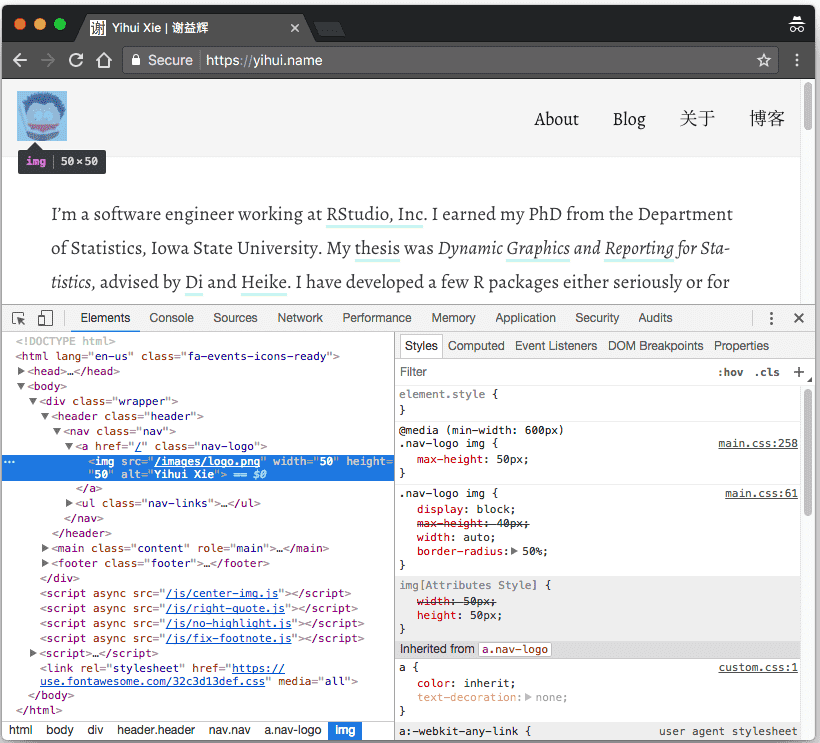
\includegraphics[width=1\linewidth]{images/chrome-devtools} 

}

\caption{Developer Tools in Google Chrome.}\label{fig:chrome-devtools}
\end{figure}

Typically you can also open the Developer Tools by right-clicking on a
certain element on the web page and selecting the menu item
\texttt{Inspect} (or \texttt{Inspect\ Element}). In Figure
\ref{fig:chrome-devtools}, I right-clicked on the profile image of my
website \url{https://yihui.name} and inspected it, and Chrome
highlighted its HTML source code
\texttt{\textless{}img\ src="..."\ ...\ /\textgreater{}} in the left
pane. You can also see the CSS styles associated with this \texttt{img}
element in the right pane. What is more, you can interactively change
the styles there if you know CSS, and see the (temporary) effects in
real time on the page! After you are satisfied with the new styles, you
can write the CSS code in files.

There are a lot of amazing features of Developer Tools, which make them
not only extremely useful for debugging and experimentation, but also
helpful for learning web development. These tools are indispensable to
me when I develop anything related to web pages. I learned a great deal
about CSS and JavaScript by playing with these tools.

\hypertarget{html}{%
\section{HTML}\label{html}}

HTML\index{HTML} stands for Hyper Text Markup Language, and it is the
language behind most web pages you see. You can use the menu
\texttt{View\ -\textgreater{}\ View\ Source} or the context menu
\texttt{View\ Page\ Source} to see the full HTML source of a web page in
your browser. All elements on a page are represented by HTML tags. For
example, the tag \texttt{\textless{}p\textgreater{}} represents
paragraphs, and \texttt{\textless{}img\textgreater{}} represents images.

The good thing about HTML is that the language has only a limited number
of tags, and the number is not very big (especially the number of
commonly used tags). This means there is hope that you can master this
language fully and quickly.

Most HTML tags appear in pairs, with an opening tag and a closing tag,
e.g., \texttt{\textless{}p\textgreater{}\textless{}/p\textgreater{}}.
You write the content between the opening and closing tags, e.g.,
\texttt{\textless{}p\textgreater{}This\ is\ a\ paragraph.\textless{}/p\textgreater{}}.
There are a few exceptions, such as the
\texttt{\textless{}img\textgreater{}} tag, which can be closed by a
slash \texttt{/} in the opening tag, e.g.,
\texttt{\textless{}img\ src="foo.png"\ /\textgreater{}}. You can specify
attributes of an element in the opening tag using the syntax
\texttt{name=value} (a few attributes do not require \texttt{value}).

HTML documents often have the filename extension \texttt{.html} (or
\texttt{.htm}). Below is an overall structure of an HTML document:

\begin{Shaded}
\begin{Highlighting}[]
\KeywordTok{<html>}

  \KeywordTok{<head>}
  \KeywordTok{</head>}
  
  \KeywordTok{<body>}
  \KeywordTok{</body>}

\KeywordTok{</html>}
\end{Highlighting}
\end{Shaded}

Basically an HTML document consists a \texttt{head} section and
\texttt{body} section. You can specify the metadata and include assets
like CSS files in the \texttt{head} section. Normally the \texttt{head}
section is not visible on a web page. It is the \texttt{body} section
that holds the content to be displayed to a reader. Below is a slightly
richer example document:

\begin{Shaded}
\begin{Highlighting}[]
\DataTypeTok{<!DOCTYPE }\NormalTok{html}\DataTypeTok{>}
\KeywordTok{<html>}

  \KeywordTok{<head>}
    \KeywordTok{<meta}\OtherTok{ charset=}\StringTok{"utf-8"} \KeywordTok{/>}
    
    \KeywordTok{<title>}\NormalTok{Your Page Title}\KeywordTok{</title>}
    
    \KeywordTok{<link}\OtherTok{ rel=}\StringTok{"stylesheet"}\OtherTok{ href=}\StringTok{"/css/style.css"} \KeywordTok{/>}
  \KeywordTok{</head>}
  
  \KeywordTok{<body>}
    \KeywordTok{<h1>}\NormalTok{A First-level Heading}\KeywordTok{</h1>}
    
    \KeywordTok{<p>}\NormalTok{A paragraph.}\KeywordTok{</p>}
    
    \KeywordTok{<img}\OtherTok{ src=}\StringTok{"/images/foo.png"}\OtherTok{ alt=}\StringTok{"A nice image"} \KeywordTok{/>}
    
    \KeywordTok{<ul>}
      \KeywordTok{<li>}\NormalTok{An item.}\KeywordTok{</li>}
      \KeywordTok{<li>}\NormalTok{Another item.}\KeywordTok{</li>}
      \KeywordTok{<li>}\NormalTok{Yet another item.}\KeywordTok{</li>}
    \KeywordTok{</ul>}
    
    \KeywordTok{<script}\OtherTok{ src=}\StringTok{"/js/bar.js"}\KeywordTok{></script>}
  \KeywordTok{</body>}

\KeywordTok{</html>}
\end{Highlighting}
\end{Shaded}

In the head, we declare the character encoding of this page to be UTF-8
via a \texttt{\textless{}meta\textgreater{}} tag, specify the title via
the \texttt{\textless{}title\textgreater{}} tag, and include a
stylesheet via a \texttt{\textless{}link\textgreater{}} tag.

The body contains a first-level section heading
\texttt{\textless{}h1\textgreater{}},\footnote{There are six possible
  levels from \texttt{h1}, \texttt{h2}, \ldots{}, to \texttt{h6}.} a
paragraph \texttt{\textless{}p\textgreater{}}, an image
\texttt{\textless{}img\textgreater{}}, an unordered list
\texttt{\textless{}ul\textgreater{}} with three list items
\texttt{\textless{}li\textgreater{}}, and includes a JavaScript file in
the end via \texttt{\textless{}script\textgreater{}}.

There are much better tutorials on HTML than this section, such as those
offered by MDN and w3schools.com, so we are not going to make this
section a full tutorial. Instead, we just want to provide a few tips on
HTML:

\begin{itemize}
\item
  You may validate your HTML code via this service:
  \url{https://validator.w3.org}. This validator will point out
  potential problems of your HTML code. It actually works for XML and
  SVG documents, too.
\item
  Among all HTML attributes, file paths (the \texttt{src} attribute of
  some tags like \texttt{\textless{}img\textgreater{}}) and links (the
  \texttt{href} attribute of the \texttt{\textless{}a\textgreater{}}
  tag) may be the most confusing to beginners. Paths and links can be
  relative or absolute, and may come with or without the protocol and
  domain. You have to understand what a link or path exactly points to.
  A full link is of the form
  \texttt{http://www.example.com/foo/bar.ext}, where \texttt{http}
  specifies the protocol (it can be other protocols like \texttt{https}
  or \texttt{ftp}), \texttt{www.example.com} is the domain, and
  \texttt{foo/bar.ext} is the file under the root directory of the
  website.

  \begin{itemize}
  \item
    If you refer to resources on the same website (the same protocol and
    domain), we recommend that you omit the protocol and domain names,
    so that the links will continue to work even if you change the
    protocol or domain. For example, a link
    \texttt{\textless{}a\ href="/hi/there.html"\textgreater{}} on a page
    \texttt{http://example.com/foo/} refers to
    \texttt{http://example.com/hi/there.html}. It does not matter if you
    change \texttt{http} to \texttt{https}, or \texttt{example.com} to
    \texttt{another-domain.com}.
  \item
    Within the same website, a link or path can be relative or absolute.
    The meaning of an absolute path does not change no matter where the
    current HTML file is placed, but the meaning of a relative path
    depends on the location of the current HTML file. Suppose you are
    currently viewing the page \texttt{example.com/hi/there.html}:

    \begin{itemize}
    \item
      A absolute path \texttt{/foo/bar.ext} always means
      \texttt{example.com/foo/bar.ext}. The leading slash means the root
      directory of the website.
    \item
      A relative path \texttt{../images/foo.png} means
      \texttt{example.com/images/foo.png} (\texttt{..} means to go one
      level up). However, if the HTML file \texttt{there.html} is moved
      to \texttt{example.com/hey/again/there.html}, this path in
      \texttt{there.html} will refer to
      \texttt{example.com/hey/images/foo.png}.
    \item
      When deciding whether to use relative or absolute paths, here is
      the rule of thumb: if you will not move the resources referred or
      linked to from one subpath to another (e.g., from
      \texttt{example.com/foo/} to \texttt{example.com/bar/}), but only
      move the HTML pages that use these resources, use absolute paths;
      if you want to change the subpath of the URL of your website, but
      the relative locations of HTML files and the resources they use do
      not change, you may use relative links (e.g., you can move the
      whole website from \texttt{example.com/} to
      \texttt{example.com/foo/}).
    \item
      If the above concepts sound too complicated, a better way is to
      either think ahead carefully about the structure of your website
      and avoid moving files, or use rules of redirects if supported
      (such as 301 or 302 redirects).
    \end{itemize}
  \item
    If you link to a different website or web page, you have to include
    the domain in the link, but it may not be necessary to include the
    protocol, e.g., \texttt{//test.example.com/foo.css} is a valid path.
    The actual protocol of this path matches the protocol of the current
    page, e.g., if the current page is \texttt{https://example.com/},
    this link means \texttt{https://test.example.com/foo.css}. It may be
    beneficial to omit the protocol because HTTP resources cannot be
    embedded on pages served through HTTPS (for security reasons), e.g.,
    an image at \texttt{http://example.com/foo.png} cannot be embedded
    on a page \texttt{https://example.com/hi.html} via
    \texttt{\textless{}img\ src="http://example.com/foo.png"\ /\textgreater{}},
    but
    \texttt{\textless{}img\ src="//example.com/foo.png"\ /\textgreater{}}
    will work if the image can be accessed via HTTPS, i.e.,
    \texttt{https://example.com/foo.png}. The main drawback of not
    including the protocol is that such links and paths do not work if
    you open the HTML file locally without using a web server, e.g.,
    only double-click the HTML file in your file browser and show it in
    the browser.\footnote{That is because without a web server, an HTML
      file is viewed via the protocol \texttt{file}. For example, you
      may see a URL of the form \texttt{file://path/to/the/file.html} in
      the address bar of your browser. The path
      \texttt{//example.com/foo.png} will be interpreted as
      \texttt{file://example.com/foo.png}, which is unlikely to exist as
      a local file on your computer.}
  \item
    A very common mistake that people make is a link without the leading
    double slashes before the domain. You may think
    \texttt{www.example.com} is a valid link. It is not! At least it
    does not link to the website that you intend to link to. It works
    when you type it in the address bar of your browser because your
    browser will normally autocomplete it to
    \texttt{http://www.example.com}. However, if you write a link
    \texttt{\textless{}a\ href="www.example.com"\textgreater{}See\ this\ link\textless{}/a\textgreater{}},
    you will be in trouble. The browser will interpret this as a
    relative link, and it is relative to the URL of the current web
    page, e.g., if you are currently viewing
    \texttt{http://yihui.name/cn/}, the link \texttt{www.example.com}
    actually means \texttt{http://yihui.name/cn/www.example.com}! Now
    you should know the Markdown text
    \texttt{{[}Link{]}(www.example.com)} is typically a mistake, unless
    you really mean to link to a subdirectory of the current page or a
    file with literally the name \texttt{www.example.com}.
  \end{itemize}
\end{itemize}

\hypertarget{css}{%
\section{CSS}\label{css}}

The Cascading Stylesheets\index{CSS} (CSS) language is used to describe
the look and formatting of documents written in HTML. CSS is responsible
for the visual style of your site. CSS is a lot of fun to play with, but
it can also easily steal your time.

In the Hugo framework
(\url{https://gohugo.io/tutorials/creating-a-new-theme/}), CSS is one of
the major ``non-content'' files that shapes the look and feel of your
site (the others are images, JavaScript, and Hugo templates). What does
the \href{https://en.wikipedia.org/wiki/Look_and_feel}{``look and
feel''} of a site mean? ``Look'' generally refers to static style
components including, but not limited to

\begin{itemize}
\tightlist
\item
  color palettes,
\item
  images,
\item
  layouts/margins, and
\item
  fonts.
\end{itemize}

whereas ``feel'' relates to dynamic components that the user interacts
with like

\begin{itemize}
\tightlist
\item
  dropdown menus,
\item
  buttons, and
\item
  forms.
\end{itemize}

There are 3 ways to define styles. The first is in line with HTML. For
example, this code

\begin{Shaded}
\begin{Highlighting}[]
\KeywordTok{<p>}\NormalTok{Marco! }\KeywordTok{<em>}\NormalTok{Polo!}\KeywordTok{</em></p>} 
\end{Highlighting}
\end{Shaded}

would produce text that looks like this: Marco! \emph{Polo!}

However, this method is generally not preferred for
\href{https://stackoverflow.com/q/12013532/559676}{numerous reasons.}

A second way is to internally define the CSS by placing a style section
in your HTML:

\begin{Shaded}
\begin{Highlighting}[]
\KeywordTok{<html>}
\KeywordTok{<style>} 
\PreprocessorTok{#favorite}\NormalTok{ \{}
    \KeywordTok{font-style}\NormalTok{: }\DecValTok{italic}\NormalTok{;}
\NormalTok{\}}
\KeywordTok{</style>}
\KeywordTok{<ul}\OtherTok{ id=}\StringTok{"tea-list"}\KeywordTok{>}
  \KeywordTok{<li>}\NormalTok{Earl Grey}\KeywordTok{</li>}
  \KeywordTok{<li>}\NormalTok{Darjeeling}\KeywordTok{</li>}
  \KeywordTok{<li>}\NormalTok{Oolong}\KeywordTok{</li>}
  \KeywordTok{<li>}\NormalTok{Chamomile}\KeywordTok{</li>}
  \KeywordTok{<li}\OtherTok{ id=}\StringTok{"favorite"}\KeywordTok{>}\NormalTok{Chai}\KeywordTok{</li>}
\KeywordTok{</ul>}
\KeywordTok{</html>}
\end{Highlighting}
\end{Shaded}

In this example, only the last tea listed, \emph{Chai}, is italicized.

The third method is the most popular because it is more flexible and the
least repetitive. In this method, you define the CSS in an external file
that is then referenced as a link in your HTML:

\begin{Shaded}
\begin{Highlighting}[]
\KeywordTok{<html>}
    \KeywordTok{<link}\OtherTok{ rel=}\StringTok{"stylesheet"}\OtherTok{ href=}\StringTok{"/css/style.css"} \KeywordTok{/>}
\KeywordTok{</html>}
\end{Highlighting}
\end{Shaded}

What goes inside the linked CSS document is essentially a list of rules
(the same list could appear internally between the style tags, if you
are using the second method). Each rule must include both a selector or
group of selectors, and a declarations block within curly braces that
contains one or more \texttt{property:\ value;} pairs. Here is the
\href{https://developer.mozilla.org/en-US/docs/Web/CSS/Reference}{general
structure for a rule}:

\begin{Shaded}
\begin{Highlighting}[]
\CommentTok{/* CSS pseudo-code */}
\NormalTok{selectorlist \{}
\NormalTok{    property: value;}
    \CommentTok{/* more property: value; pairs*/}
\NormalTok{\}}
\end{Highlighting}
\end{Shaded}

\href{https://developer.mozilla.org/en-US/docs/Web/CSS/Reference\#Selectors}{Selectors}
can be based on HTML element types or attributes, such as \texttt{id} or
\texttt{class} (and combinations of these attributes):

\begin{Shaded}
\begin{Highlighting}[]
\CommentTok{/* by element type */}
\NormalTok{li \{ }
    \KeywordTok{color}\NormalTok{: }\DecValTok{yellow}\NormalTok{; }\CommentTok{/* all <li> elements are yellow */}
\NormalTok{\}}

\CommentTok{/* by ID with the # symbol */}
\PreprocessorTok{#my-id}\NormalTok{ \{ }
    \KeywordTok{color}\NormalTok{: }\DecValTok{yellow}\NormalTok{; }\CommentTok{/* elements with id = "my-id" are yellow */}
\NormalTok{\}}

\CommentTok{/* by class with the . symbol */}
\FunctionTok{.my-class}\NormalTok{ \{ }
    \KeywordTok{color}\NormalTok{: }\DecValTok{yellow}\NormalTok{; }\CommentTok{/* elements with class = "my-class" are yellow  */}
\NormalTok{\}}
\end{Highlighting}
\end{Shaded}

Because each HTML element may match several different selectors, the CSS
standard determines which set of rules has precedence for any given
element, and which properties to inherit. This is where the cascade
algorithm comes into play. For example, take a simple unordered list:

\begin{Shaded}
\begin{Highlighting}[]
\KeywordTok{<ul}\OtherTok{ id=}\StringTok{"tea-list"}\KeywordTok{>}
  \KeywordTok{<li>}\NormalTok{Earl Grey}\KeywordTok{</li>}
  \KeywordTok{<li>}\NormalTok{Darjeeling}\KeywordTok{</li>}
  \KeywordTok{<li>}\NormalTok{Oolong}\KeywordTok{</li>}
  \KeywordTok{<li>}\NormalTok{Chamomile}\KeywordTok{</li>}
  \KeywordTok{<li>}\NormalTok{Chai}\KeywordTok{</li>}
\KeywordTok{</ul>}
\end{Highlighting}
\end{Shaded}

Now, let's say we want to highlight our favorite teas again, so we'll
use a class attribute.

\begin{Shaded}
\begin{Highlighting}[]
\KeywordTok{<ul}\OtherTok{ id=}\StringTok{"tea-list"}\KeywordTok{>}
  \KeywordTok{<li>}\NormalTok{Earl Grey}\KeywordTok{</li>}
  \KeywordTok{<li}\OtherTok{ class=}\StringTok{"favorite"}\KeywordTok{>}\NormalTok{Darjeeling}\KeywordTok{</li>}
  \KeywordTok{<li>}\NormalTok{Oolong}\KeywordTok{</li>}
  \KeywordTok{<li>}\NormalTok{Chamomile}\KeywordTok{</li>}
  \KeywordTok{<li}\OtherTok{ class=}\StringTok{"favorite"}\KeywordTok{>}\NormalTok{Chai}\KeywordTok{</li>}
\KeywordTok{</ul>}
\end{Highlighting}
\end{Shaded}

We can use this class attribute as a selector in our CSS. Let's say we
want our favorite teas to be in bold and have a background color of
yellow, so our CSS would look like this:

\begin{Shaded}
\begin{Highlighting}[]
\FunctionTok{.favorite}\NormalTok{ \{}
  \KeywordTok{font-weight}\NormalTok{: }\DecValTok{bold}\NormalTok{;}
  \KeywordTok{background-color}\NormalTok{: }\DecValTok{yellow}\NormalTok{;}
\NormalTok{\}}
\end{Highlighting}
\end{Shaded}

Now, if you want every list item to be italicized with a white
background, you can set up another rule:

\begin{Shaded}
\begin{Highlighting}[]
\NormalTok{li \{ }
  \KeywordTok{font-style}\NormalTok{: }\DecValTok{italic}\NormalTok{;}
  \KeywordTok{background-color}\NormalTok{: }\DecValTok{white}\NormalTok{;}
\NormalTok{\}}
\end{Highlighting}
\end{Shaded}

If you play with this code (which you can do easily using sites like
\url{http://jsbin.com}, \url{https://jsfiddle.net}, or
\url{https://codepen.io/pen/}), you'll see that the two favorite teas
are still highlighted in yellow. This is because the CSS rule about
\texttt{.favorite} as a class is more specific than the rule about
\texttt{li} type elements. To override the \texttt{.favorite} rule, you
need to be as specific as you can be when choosing your group of
selectors:

\begin{Shaded}
\begin{Highlighting}[]
\NormalTok{ul}\PreprocessorTok{#tea-list}\NormalTok{ li}\FunctionTok{.favorite}\NormalTok{ \{}
  \KeywordTok{background-color}\NormalTok{: }\DecValTok{white}\NormalTok{;}
\NormalTok{\}}
\end{Highlighting}
\end{Shaded}

This example just scratches the surface of
\href{https://developer.mozilla.org/en-US/docs/Learn/CSS/Introduction_to_CSS/Cascade_and_inheritance}{cascade
and inheritance.}

For any Hugo theme that you install, you can find the CSS file in the
\texttt{themes/} folder. For example, the default lithium theme is
located in: \texttt{themes/hugo-lithium-theme/static/css/main.css}. Once
you are familiar with CSS, you can understand how each set of rules work
to shape the visual style of your website, and how to alter the rules.
For some themes (i.e., the
\href{https://github.com/gcushen/hugo-academic}{hugo-academic theme}),
you have the option of linking to a
\href{https://gist.github.com/gcushen/d5525a4506b9ccf83f2bce592a895495}{custom
CSS,} which you can use to further customize the visual style of your
site.

A few one-line examples illustrate how simple CSS rules can be used to
make dramatic changes:

\begin{itemize}
\item
  To make circular or rounded images, you may assign a class
  \texttt{img-circle} to images (e.g.,
  \texttt{\textless{}img\ class="img-circle"\ src="foo.png"\ /\textgreater{}})
  and define the CSS:

\begin{Shaded}
\begin{Highlighting}[]
\FunctionTok{.img-circle}\NormalTok{ \{}
  \KeywordTok{border-radius}\NormalTok{: }\DecValTok{50%}\NormalTok{;}
\NormalTok{\}}
\end{Highlighting}
\end{Shaded}
\item
  To make striped tables, you can add background colors to odd or even
  rows of the table, e.g.,

\begin{Shaded}
\begin{Highlighting}[]
\NormalTok{tr}\InformationTok{:nth-child}\NormalTok{(even) \{}
  \KeywordTok{background}\NormalTok{: }\DecValTok{#eee}\NormalTok{;}
\NormalTok{\}}
\end{Highlighting}
\end{Shaded}
\item
  You can append or prepend content to elements via pseudo-elements
  \texttt{::after} and \texttt{::before}. Here is an example of adding a
  period after section numbers:
  \url{https://github.com/rstudio/blogdown/issues/80}.
\end{itemize}

\hypertarget{javascript}{%
\section{JavaScript}\label{javascript}}

It is way more challenging to briefly introduce
JavaScript\index{JavaScript} than HTML and CSS, since it is a
programming language. There are many books and tutorials about this
language. Anyway, we will try to scratch the surface for R users in this
section.

In a nutshell, JavaScript is a language that is typically used to
manipulate elements on a web page. An effective way to learn it is
through the JavaScript console in the Developer Tools of your web
browser (see Figure \ref{fig:chrome-devtools}), because you can
interactively type code in the console and execute it, which feels
similar to executing R code in the R console (e.g., in RStudio). You may
open any web page in your web browser (e.g., \url{https://yihui.name}),
then open the JavaScript console, and try the code below on any web
page:

\begin{Shaded}
\begin{Highlighting}[]
\VariableTok{document}\NormalTok{.}\VariableTok{body}\NormalTok{.}\VariableTok{style}\NormalTok{.}\AttributeTok{background} \OperatorTok{=} \StringTok{'orange'}\OperatorTok{;}
\end{Highlighting}
\end{Shaded}

It should change the background color of the page to orange, unless the
page has already defined background colors for certain elements.

To effectively use JavaScript, you have to learn both the basic syntax
of JavaScript and how to select elements on a page before you can
manipulate them. You may partially learn the former from the short
JavaScript snippet below:

\begin{Shaded}
\begin{Highlighting}[]
\KeywordTok{var}\NormalTok{ x }\OperatorTok{=} \DecValTok{1}\OperatorTok{;}  \CommentTok{// assignments}
\DecValTok{1} \OperatorTok{+} \DecValTok{2} \OperatorTok{-} \DecValTok{3} \OperatorTok{*} \DecValTok{4}\NormalTok{ / }\DecValTok{5}\OperatorTok{;}  \CommentTok{// arithmetic}

\ControlFlowTok{if}\NormalTok{ (x }\OperatorTok{<} \DecValTok{2}\NormalTok{) }\VariableTok{console}\NormalTok{.}\AttributeTok{log}\NormalTok{(x)}\OperatorTok{;}  \CommentTok{// "print" x}

\KeywordTok{var}\NormalTok{ y }\OperatorTok{=}\NormalTok{ [}\DecValTok{9}\OperatorTok{,} \DecValTok{1}\OperatorTok{,} \DecValTok{0}\OperatorTok{,} \DecValTok{2}\OperatorTok{,} \DecValTok{1}\OperatorTok{,} \DecValTok{4}\NormalTok{]}\OperatorTok{;}  \CommentTok{// array}

\CommentTok{// function}
\KeywordTok{var}\NormalTok{ sum }\OperatorTok{=} \KeywordTok{function}\NormalTok{(x) }\OperatorTok{\{}
  \KeywordTok{var}\NormalTok{ s }\OperatorTok{=} \DecValTok{0}\OperatorTok{;}
  \CommentTok{// a naive way to compute the sum}
  \ControlFlowTok{for}\NormalTok{ (}\KeywordTok{var}\NormalTok{ i}\OperatorTok{=}\DecValTok{0}\OperatorTok{;}\NormalTok{ i }\OperatorTok{<} \VariableTok{x}\NormalTok{.}\AttributeTok{length}\OperatorTok{;}\NormalTok{ i}\OperatorTok{++}\NormalTok{) }\OperatorTok{\{}
\NormalTok{    s }\OperatorTok{+=}\NormalTok{ x[i]}\OperatorTok{;}
  \OperatorTok{\}}
  \ControlFlowTok{return}\NormalTok{ s}\OperatorTok{;}
\OperatorTok{\};}

\AttributeTok{sum}\NormalTok{(y)}\OperatorTok{;}

\KeywordTok{var}\NormalTok{ y }\OperatorTok{=} \StringTok{"Hello World"}\OperatorTok{;}
\NormalTok{y }\OperatorTok{=} \VariableTok{y}\NormalTok{.}\AttributeTok{replace}\NormalTok{(}\StringTok{" "}\OperatorTok{,} \StringTok{", "}\NormalTok{)}\OperatorTok{;}  \CommentTok{// string manipulation}
\end{Highlighting}
\end{Shaded}

You may feel the syntax is similar to R to some degree. JavaScript is an
object-oriented language, and usually there are several methods that you
can apply to an object. The string manipulation above is a typical
example of the \texttt{Object.method()} syntax. To know the possible
methods on an object, you can type the object name in your JavaScript
console followed by a dot, and you should see all candidates.

R users have to be extremely cautious because JavaScript objects are
often mutable, meaning that an object could be modified anywhere. Below
is a quick example:

\begin{Shaded}
\begin{Highlighting}[]
\KeywordTok{var}\NormalTok{ x }\OperatorTok{=} \OperatorTok{\{}\StringTok{"a"}\OperatorTok{:} \DecValTok{1}\OperatorTok{,} \StringTok{"b"}\OperatorTok{:} \DecValTok{2}\OperatorTok{\};}  \CommentTok{// like a list in R}
\KeywordTok{var}\NormalTok{ f }\OperatorTok{=} \KeywordTok{function}\NormalTok{(z) }\OperatorTok{\{}
  \VariableTok{z}\NormalTok{.}\AttributeTok{a} \OperatorTok{=} \DecValTok{100}\OperatorTok{;}
\OperatorTok{\};}
\AttributeTok{f}\NormalTok{(x)}\OperatorTok{;}
\NormalTok{x}\OperatorTok{;}  \CommentTok{// modified! x.a is 100 now}
\end{Highlighting}
\end{Shaded}

There are many mature JavaScript libraries that can help you select and
manipulate elements on a page, and the most popular one may
be\index{jQuery} \href{https://jquery.com}{jQuery.} However, you should
know that sometimes you can probably do well enough without these
third-party libraries. There are some basic methods to select elements,
such as \texttt{document.getElementById()} and
\texttt{document.getElementsByClassName()}. For example, you can select
all paragraphs using
\texttt{document.querySelectorAll(\textquotesingle{}p\textquotesingle{})}.

Next we show a slightly advanced application, in which you will see
anonymous functions, selection of elements by HTML tag names, regular
expressions, and manipulation of HTML elements.

In Section \ref{how-to}, we mentioned how to enable
MathJax\index{MathJax} on a Hugo website. The easy part is to include
the script \texttt{MathJax.js} via a
\texttt{\textless{}script\textgreater{}} tag, and there are two hard
parts:

\begin{enumerate}
\def\labelenumi{\arabic{enumi}.}
\item
  How to protect the math content from the Markdown engine
  (Blackfriday), e.g., we need to make sure underscores in math
  expressions are not interpreted as
  \texttt{\textless{}em\textgreater{}\textless{}/em\textgreater{}}. This
  problem only exists in plain Markdown posts, and has been mentioned in
  Section \ref{output-format} without explaining the solution.
\item
  By default, MathJax does not recognize a pair of single dollar signs
  as the syntax for inline math expressions, but most users are perhaps
  more comfortable with the syntax \texttt{\$x\$} than
  \texttt{\textbackslash{}(x\textbackslash{})}.
\end{enumerate}

The easiest solution to the first problem may be adding backticks around
math expressions, e.g.,
\texttt{\textasciigrave{}\$x\_i\$\textasciigrave{}}, but the consequence
is that the math expression will be rendered in
\texttt{\textless{}code\textgreater{}\textless{}/code\textgreater{}},
and MathJax ignores \texttt{\textless{}code\textgreater{}} tags when
looking for math expressions on the page. We can force MathJax to search
for math expressions in \texttt{\textless{}code\textgreater{}}, but this
will still be problematic. For example, someone may want to display
inline R code \texttt{\textasciigrave{}list\$x\$y\textasciigrave{}}, and
\texttt{\$x\$} may be recognized as a math expression. MathJax ignores
\texttt{\textless{}code\textgreater{}} for good reasons. Even if you do
not have such expressions in \texttt{\textless{}code\textgreater{}}, you
may have some special CSS styles attached to
\texttt{\textless{}code\textgreater{}}, and these styles will be applied
to your math expressions, which can be undesired (e.g., a light gray
background).

To solve these problems, I have provided a solution in the JavaScript
code at \url{https://yihui.name/js/math-code.js}:

\begin{Shaded}
\begin{Highlighting}[]
\NormalTok{(}\KeywordTok{function}\NormalTok{() }\OperatorTok{\{}
  \KeywordTok{var}\NormalTok{ i}\OperatorTok{,}\NormalTok{ text}\OperatorTok{,}\NormalTok{ code}\OperatorTok{,}\NormalTok{ codes }\OperatorTok{=} \VariableTok{document}\NormalTok{.}\AttributeTok{getElementsByTagName}\NormalTok{(}\StringTok{'code'}\NormalTok{)}\OperatorTok{;}
  \ControlFlowTok{for}\NormalTok{ (i }\OperatorTok{=} \DecValTok{0}\OperatorTok{;}\NormalTok{ i }\OperatorTok{<} \VariableTok{codes}\NormalTok{.}\AttributeTok{length}\OperatorTok{;}\NormalTok{) }\OperatorTok{\{}
\NormalTok{    code }\OperatorTok{=}\NormalTok{ codes[i]}\OperatorTok{;}
    \ControlFlowTok{if}\NormalTok{ (}\VariableTok{code}\NormalTok{.}\VariableTok{parentNode}\NormalTok{.}\AttributeTok{tagName} \OperatorTok{!==} \StringTok{'PRE'} \OperatorTok{&&}
        \VariableTok{code}\NormalTok{.}\AttributeTok{childElementCount} \OperatorTok{===} \DecValTok{0}\NormalTok{) }\OperatorTok{\{}
\NormalTok{      text }\OperatorTok{=} \VariableTok{code}\NormalTok{.}\AttributeTok{textContent}\OperatorTok{;}
      \ControlFlowTok{if}\NormalTok{ (}\SpecialStringTok{/}\SpecialCharTok{^\textbackslash{}$[^$]}\SpecialStringTok{/}\NormalTok{.}\AttributeTok{test}\NormalTok{(text) }\OperatorTok{&&} \SpecialStringTok{/}\SpecialCharTok{[^$]\textbackslash{}$$}\SpecialStringTok{/}\NormalTok{.}\AttributeTok{test}\NormalTok{(text)) }\OperatorTok{\{}
\NormalTok{        text }\OperatorTok{=} \VariableTok{text}\NormalTok{.}\AttributeTok{replace}\NormalTok{(}\SpecialStringTok{/}\SpecialCharTok{^\textbackslash{}$}\SpecialStringTok{/}\OperatorTok{,} \StringTok{'}\SpecialCharTok{\textbackslash{}\textbackslash{}}\StringTok{('}\NormalTok{).}\AttributeTok{replace}\NormalTok{(}\SpecialStringTok{/}\SpecialCharTok{\textbackslash{}$$}\SpecialStringTok{/}\OperatorTok{,} \StringTok{'}\SpecialCharTok{\textbackslash{}\textbackslash{}}\StringTok{)'}\NormalTok{)}\OperatorTok{;}
        \VariableTok{code}\NormalTok{.}\AttributeTok{textContent} \OperatorTok{=}\NormalTok{ text}\OperatorTok{;}
      \OperatorTok{\}}
      \ControlFlowTok{if}\NormalTok{ (}\SpecialStringTok{/}\SpecialCharTok{^\textbackslash{}\textbackslash{}\textbackslash{}((}\SpecialStringTok{.}\SpecialCharTok{|\textbackslash{}s)+\textbackslash{}\textbackslash{}\textbackslash{})$}\SpecialStringTok{/}\NormalTok{.}\AttributeTok{test}\NormalTok{(text) }\OperatorTok{||}
          \SpecialStringTok{/}\SpecialCharTok{^\textbackslash{}\textbackslash{}\textbackslash{}[(}\SpecialStringTok{.}\SpecialCharTok{|\textbackslash{}s)+\textbackslash{}\textbackslash{}\textbackslash{}]$}\SpecialStringTok{/}\NormalTok{.}\AttributeTok{test}\NormalTok{(text) }\OperatorTok{||}
          \SpecialStringTok{/}\SpecialCharTok{^\textbackslash{}$(}\SpecialStringTok{.}\SpecialCharTok{|\textbackslash{}s)+\textbackslash{}$$}\SpecialStringTok{/}\NormalTok{.}\AttributeTok{test}\NormalTok{(text) }\OperatorTok{||}
          \SpecialStringTok{/}\SpecialCharTok{^\textbackslash{}\textbackslash{}}\SpecialStringTok{begin}\SpecialCharTok{\textbackslash{}\{([^\}]+)\textbackslash{}\}(}\SpecialStringTok{.}\SpecialCharTok{|\textbackslash{}s)+\textbackslash{}\textbackslash{}}\SpecialStringTok{end}\SpecialCharTok{\textbackslash{}\{[^\}]+\textbackslash{}\}$}\SpecialStringTok{/}\NormalTok{.}\AttributeTok{test}\NormalTok{(text)) }\OperatorTok{\{}
        \VariableTok{code}\NormalTok{.}\AttributeTok{outerHTML} \OperatorTok{=} \VariableTok{code}\NormalTok{.}\AttributeTok{innerHTML}\OperatorTok{;}  \CommentTok{// remove <code></code>}
        \ControlFlowTok{continue}\OperatorTok{;}
      \OperatorTok{\}}
    \OperatorTok{\}}
\NormalTok{    i}\OperatorTok{++;}
  \OperatorTok{\}}
\OperatorTok{\}}\NormalTok{)()}\OperatorTok{;}
\end{Highlighting}
\end{Shaded}

It is not a perfect solution, but it should be very rare that you run
into problems. This solution identifies possible math expressions in
\texttt{\textless{}code\textgreater{}}, and strips the
\texttt{\textless{}code\textgreater{}} tag, e.g., replaces
\texttt{\textless{}code\textgreater{}\$x\$\textless{}/code\textgreater{}}
with \texttt{\textbackslash{}(x\textbackslash{})}. After this script is
executed, we load the MathJax script. This way, we do not need to force
MathJax to search for math expressions in
\texttt{\textless{}code\textgreater{}} tags, and your math expressions
will not inherit any styles from \texttt{\textless{}code\textgreater{}}.
The JavaScript code above is not too long, and should be
self-explanatory. The trickiest part is \texttt{i++}. I will leave it to
readers to figure out why the \texttt{for} loop is not the usual form
\texttt{for\ (i\ =\ 0;\ i\ \textless{}\ codes.length;\ i++)}. It took me
quite a few minutes to realize my mistake when I wrote the loop in the
usual form.

\hypertarget{useful-resources}{%
\section{Useful resources}\label{useful-resources}}

\hypertarget{file-optimization}{%
\subsection{File optimization}\label{file-optimization}}

Although\index{Optimization} static websites are fast in general, you
can certainly further optimize them. You may search for ``CSS and
JavaScript minifier,'' and these tools can compress your CSS and
JavaScript files, so that they can be loaded faster. Since there are a
lot of tools, I will not recommend any here.

You can also optimize images on your website. I frequently use a
command-line tool named
\href{http://optipng.sourceforge.net}{\texttt{optipng}} to optimize PNG
images. It is a lossless optimizer, meaning that it reduces the file
size of a PNG image without loss of quality. From my experience, it
works very well on PNG images generated from R, and can reduce the file
size by at least 30\% (sometimes even more than 50\%). Personally I also
use online tools like \url{http://optimizilla.com} to optimize PNG and
JPEG images. For GIF images, I often use
\url{https://ezgif.com/optimize} to reduce the file sizes if they are
too big.

Note that Netlify has provided the optimization features on the server
side for free at the moment, so you may just want to enable them there
instead of doing all the hard work by yourself.

\hypertarget{helping-people-find-your-site}{%
\subsection{Helping people find your
site}\label{helping-people-find-your-site}}

Once your site is up and running, you probably want people to find it.
SEO --- Search Engine Optimization --- is the art of making a website
easy for search engines like Google to understand. And, hopefully, if
the search engine knows what you are writing about, it will present
links to your site high in results when someone searches for topics you
cover.

Entire books have been written about SEO, not to mention the many
companies that are in the business of offering (paid) technical and
strategic advice to help get sites atop search-engine rankings. If you
are interested in finding out more, a good place to start is the Google
Search Engine Optimization Starter Guide
(\url{http://bit.ly/google-seo-starter}). Below are a few key points:

\begin{enumerate}
\def\labelenumi{\arabic{enumi}.}
\item
  The title that you select for each page and post is a very important
  signal to Google and other search engines telling them what that page
  is about.
\item
  Description tags are also critical to explain what a page is about. In
  HTML documents,
  \href{https://www.w3schools.com/tags/tag_meta.asp}{description tags}
  are one way to provide metadata about the page. Using
  \textbf{blogdown}, the description may end up as text under the page
  title in a search-engine result. If your page's YAML does not include
  a description, you can add one like
  \texttt{description:\ "A\ brief\ description\ of\ this\ page."}; the
  HTML source of the rendered page would have a
  \texttt{\textless{}meta\textgreater{}} tag in
  \texttt{\textless{}head\textgreater{}} like
  \texttt{\textless{}meta\ name="description"\ content="A\ brief\ description\ of\ this\ page."\textgreater{}}.
  Not all themes support adding the description to your HTML page
  (although they should!)
\item
  URL structure also matters. You want your post's slug to have
  informative keywords, which gives another signal of what the page is
  about. Have a post with interesting things to do in San Francisco?
  \texttt{san-francisco-events-calendar} might be a better slug than
  \texttt{my-guide-to-fun-things-to-do}.
\end{enumerate}

\hypertarget{domain-name}{%
\chapter{Domain Name}\label{domain-name}}

While you can use the free subdomain names\index{Domain Name} like those
provided by GitHub or Netlify, it may be a better idea to own a domain
name of your own. The cost of an apex domain is minimal (typically the
yearly cost is about US\$10), and you will enter a much richer world
after you purchase a domain name. For example, you are free to point
your domain to any web servers, you can create as many subdomain names
as you want, and you can even set up your own email accounts using the
domain or subdomains. In this appendix, we will explain some basic
concepts of domain names, and mention a few (free) services to help you
configure your domain name.

Before we dive into the details, we want to outline the big picture of
how a URL works in your web browser. Suppose you typed or clicked a link
\texttt{http://www.example.com/foo/index.html} in your web browser. What
happens behind the scenes before you see the actual web page?

First, the domain name has to be resolved through the nameservers
associated with it. A nameserver knows the DNS (Domain Name System)
records of a domain. Typically it will look up the ``A records'' to
point the domain to the IP address of a web server. There are several
other types of DNS records, and we will explain them later. Once the web
server is reached, the server will look for the file
\texttt{foo/index.html} under a directory associated with the domain
name, and return its content in the response. That is basically how you
can see a web page.

\hypertarget{registration}{%
\section{Registration}\label{registration}}

You can purchase a domain name from many domain name registrars. To stay
neutral, we are not going to make recommendations here. You can use your
search engine to find a registrar by yourself, or ask your friends for
recommendations. However, we would like to remind you of a few things
that you should pay attention to when looking for a domain name
registrar:

\begin{itemize}
\item
  You should have the freedom to transfer your domain from the current
  registrar to other registrars, i.e., they should not lock you in their
  system. To transfer a domain name, you should be given a code known as
  the ``Transfer Auth Code'' or ``Auth Code'' or ``Transfer Key'' or
  something like that.
\item
  You should be able to customize the nameservers (see Section
  \ref{nameservers}) of your domain. By default, each registrar will
  assign their own nameservers to you, and these nameservers typically
  work very well. However, there are some special nameservers that
  provide services more than just DNS records, and you may be interested
  in using them.
\item
  Other people can freely look up your personal information, such as
  your email or postal address, after you register a domain and submit
  this information to the registrar. This is called the ``WHOIS
  Lookup.'' You may want to protect your privacy, but your registrar may
  require an extra payment.
\end{itemize}

\hypertarget{nameservers}{%
\section{Nameservers}\label{nameservers}}

The main reason why we need nameservers\index{Nameservers} is that we
want to use domains instead of IP addresses, although a domain is not
strictly necessary for you to be able to access a website. You could use
the IP address if you have your own server with a public IP, but there
are many problems with this approach. For example, IP addresses are
limited (in particular IPv4), not easy to memorize, and you can only
host one website per IP address (without using other ports).

A nameserver is an engine that directs the DNS records of your domain.
The most common DNS record is the A record, which maps a domain to an IP
address, so that the hosting server can be found via its IP address when
a website is accessed through a domain. We will introduce two more types
of DNS records in Section \ref{dns-records}: CNAME and MX records.

In most cases, the default nameservers provided by your domain registrar
should suffice, but there is a special technology missing in most
nameservers: CNAME flattening. You only need this technology if you want
to set a CNAME record for your apex domain. The only use case to my
knowledge is when you host your website via Netlify, but want to use the
apex domain instead of the \texttt{www} subdomain, e.g., you want to use
\texttt{example.com} instead of \texttt{www.example.com}. To make use of
this technology, you could consider
\href{https://www.cloudflare.com}{Cloudflare,} which provides this DNS
feature for free. Basically, all you need to do is to point the
nameservers of your domain to the nameservers provided by Cloudflare (of
the form \texttt{*.ns.cloudflare.com}).

\hypertarget{dns-records}{%
\section{DNS records}\label{dns-records}}

There are many types of DNS\index{DNS Records} records, and you may see
a full list on
\href{https://en.wikipedia.org/wiki/List_of_DNS_record_types}{Wikipedia.}
The most commonly used types may be A, CNAME, and MX records. Figure
\ref{fig:cloudflare-dns} shows a subset of DNS records of my domain
\texttt{yihui.name} on Cloudflare, which may give you an idea of what
DNS records look like. You may query DNS records using command-line
tools such as
\href{https://en.wikipedia.org/wiki/Dig_(command)}{\texttt{dig}} or an
app provided by Google: \url{https://toolbox.googleapps.com/apps/dig/}.

\begin{figure}

{\centering 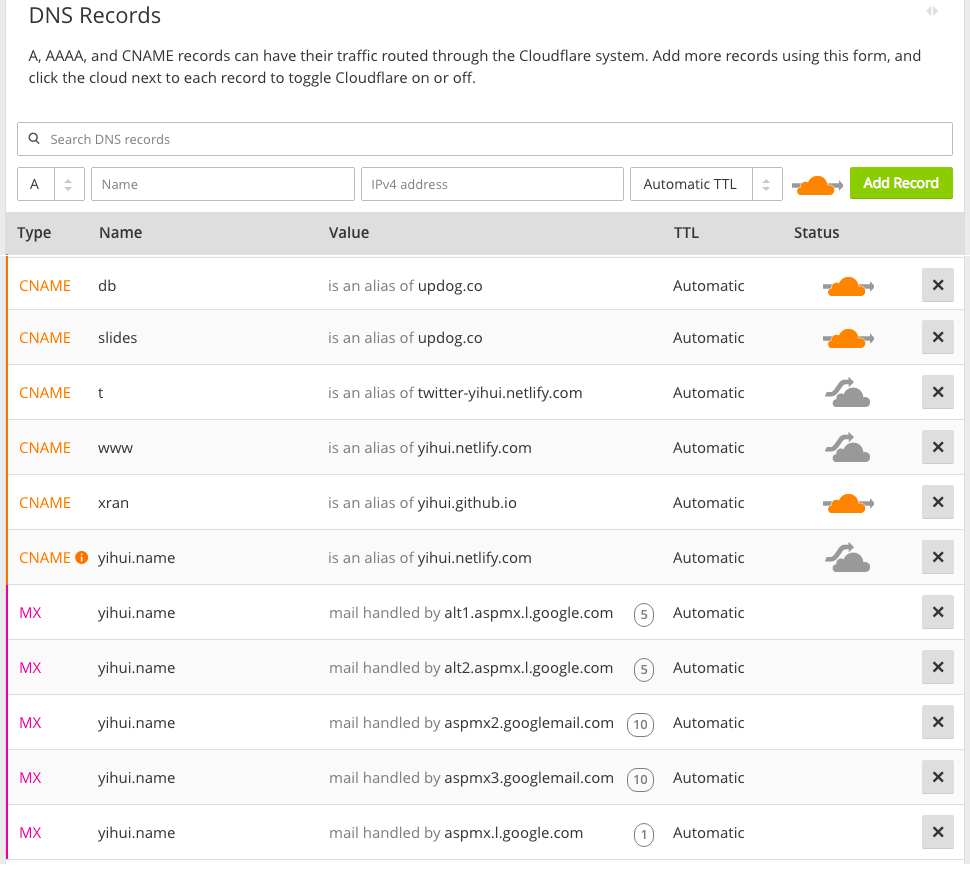
\includegraphics[width=1\linewidth]{images/cloudflare-dns} 

}

\caption{Some DNS records of the domain yihui.name on Cloudflare.}\label{fig:cloudflare-dns}
\end{figure}

An apex domain can have any number of subdomains. You can set DNS
records for the apex domain and any subdomains. You can see from Figure
\ref{fig:cloudflare-dns} that I have several subdomains, e.g.,
\texttt{slides.yihui.name} and \texttt{xran.yihui.name}.

As we have mentioned, an A record points a domain or subdomain to an IP
address of the host server. I did not use any A records for my domains
since all services I use, such as Updog, GitHub Pages, and Netlify,
support CNAME records well. A CNAME\index{CNAME Record} record is an
alias, pointing one domain to another domain. The advantage of using
CNAME over A is that you do not have to tie a domain to a fixed IP
address. For example, the CNAME record for \texttt{t.yihui.name} is
\texttt{twitter-yihui.netlify.com}. The latter domain is provided by
Netlify, and I do not need to know where they actually host the website.
They are free to move the host of \texttt{twitter-yihui.netlify.com},
and I will not need to update my DNS record. Every time someone visits
the website \texttt{t.yihui.name}, the web browser will route the
traffic to the domain set in the CNAME record. Note that this is
different from redirection, i.e., the URL \texttt{t.yihui.name} will not
be explicitly redirected to \texttt{twitter-yihui.netlify.com} (you
still see the former in the address bar of your browser).

Normally, you can set any DNS records for the apex domain except CNAME,
but I set a CNAME record for my apex domain \texttt{yihui.name}, and
that is because Cloudflare supports CNAME flattening. For more
information on this topic, you may read the post
\href{https://www.netlify.com/blog/2017/02/28/to-www-or-not-www/}{``To
WWW or not WWW,''} by Netlify. Personally, I prefer not using the
subdomain \texttt{www.yihui.name} to keep my URLs short, so I set a
CNAME record for both the apex domain \texttt{yihui.name} and the
\texttt{www} subdomain, and Netlify will automatically redirect the
\texttt{www} subdomain to the apex domain. That said, if you are a
beginner, it may be a little easier to configure and use the
\texttt{www} subdomain, as suggested by Netlify. Note \texttt{www} is a
conventional subdomain that sounds like an apex domain, but really is
not; you can follow this convention or not as you wish.

For email services, I was an early enough
\href{https://en.wikipedia.org/wiki/Netizen}{``netizen'',} and when I
registered my domain name, Google was still offering free email services
to custom domain owners. That is how I can have a custom mailbox
\texttt{xie@yihui.name}. Now you will have to pay for
\href{https://gsuite.google.com}{G Suite.} In Figure
\ref{fig:cloudflare-dns} you can see I have set some MX (stands for
``mail exchange'') records that point to some Google mail servers. Of
course, Google is not the only possible choice when it comes to custom
mailboxes. \href{https://www.migadu.com}{Migadu} claims to be the ``most
affordable email hosting.'' You may try its free plan and see if you
like it. Unless you are going to use your custom mailbox extensively and
for professional purposes, the free plan may suffice. In fact, you may
create an alias address on Migadu to forward emails to your other email
accounts (such as Gmail) if you do not care about an actual custom
mailbox. Migadu has provided detailed instructions on how to set the MX
records for your domain.

\hypertarget{advanced-topics}{%
\chapter{Advanced Topics}\label{advanced-topics}}

In this appendix, we talk about a few advanced topics that may be of
interest to developers and advanced users.

\hypertarget{more-global-options}{%
\section{More global options}\label{more-global-options}}

There are a few more advanced global options\index{Global Options} in
addition to those introduced in Section \ref{global-options}, and they
are listed in Table \ref{tab:global-options2}.

\begin{table}

\caption{\label{tab:global-options2}A few more advanced global options.}
\centering
\begin{tabular}[t]{lll}
\toprule
Option name & Default & Meaning\\
\midrule
blogdown.hugo.dir &  & The directory of the Hugo executable\\
blogdown.method & html & The building method for R Markdown\\
blogdown.publishDir &  & The publish dir for local preview\\
blogdown.widgetsID & TRUE & Incremental IDs for HTML widgets?\\
\bottomrule
\end{tabular}
\end{table}

If you want to install Hugo to a custom path, you can set the global
option \texttt{blogdown.hugo.dir} to a directory to store the Hugo
executable before you call \texttt{install\_hugo()}, e.g.,
\texttt{options(blogdown.hugo.dir\ =\ \textquotesingle{}\textasciitilde{}/Downloads/hugo\_0.20.1/\textquotesingle{})}.
This may be useful for you to use a specific version of Hugo for a
specific website,\footnote{You can set this option per project. See
  Section \ref{global-options} for details.} or store a copy of Hugo on
a USB Flash drive along with your website.

The option \texttt{blogdown.method} is explained in Section
\ref{methods}.

When your website project is under version control in the RStudio IDE,
continuously previewing the site can be slow, if it contains hundreds of
files or more. The default publish directory is \texttt{public/} under
the project root directory, and whenever you make a change in the source
that triggers a rebuild, RStudio will be busy tracking file changes in
the \texttt{public/} directory. The delay before you see the website in
the RStudio Viewer can be 10 seconds or even longer. That is why we
provide the option \texttt{blogdown.publishDir}. You may set a temporary
publish directory to generate the website, and this directory should not
be under the same RStudio project, e.g.,
\texttt{options(blogdown.publishDir\ =\ \textquotesingle{}../public\_site\textquotesingle{})},
which means the website will be generated to the directory
\texttt{public\_site/} under the parent directory of the current
project.

The option \texttt{blogdown.widgetsID} is only relevant if your website
source is under version control and you have HTML widgets on the
website. If this option is \texttt{TRUE} (default), the random IDs of
HTML widgets will be changed to incremental IDs in the HTML output, so
these IDs are unlikely to change every time you recompile your website;
otherwise, every time you will get different random IDs.

\hypertarget{livereload}{%
\section{LiveReload}\label{livereload}}

As we briefly mentioned\index{LiveReload} in Section
\ref{a-quick-example}, you can use \texttt{blogdown::serve\_site()} to
preview a website, and the web page will be automatically rebuilt and
reloaded in your web browser when the source file is modified and saved.
This is called ``LiveReload.''

We have provided two approaches to LiveReload. The default approach is
through \texttt{servr::httw()}, which will continuously watch the
website directory for file changes, and rebuild the site when changes
are detected. This approach has a few drawbacks:

\begin{enumerate}
\def\labelenumi{\arabic{enumi}.}
\item
  It is relatively slow because the website is fully regenerated every
  time. This may not be a real problem for Hugo, because Hugo is often
  fast enough: it takes about a millisecond to generate one page, so a
  website with a thousand pages may only take about one second to be
  fully regenerated.
\item
  The daemonized server (see Section \ref{global-options}) may not work.
\end{enumerate}

If you are not concerned about the above issues, we recommend that you
use the default approach, otherwise you can set the global option
\texttt{options(blogdown.generator.server\ =\ TRUE)} to use an
alternative approach to LiveReload, which is based on the native support
for LiveReload from the static site generator. At the moment, this has
only been tested against Hugo-based websites. It does not work with
Jekyll and we were not successful with Hexo, either.

This alternative approach requires two additional R packages to be
installed: \textbf{processx} \citep{R-processx} and \textbf{later}
\citep{R-later}. You may use this approach when you primarily work on
plain Markdown posts instead of R Markdown posts, because it can be much
faster to preview Markdown posts using the web server of Hugo. The web
server can be stopped by \texttt{blogdown::stop\_server()}, and it will
always be stopped when the R session is ended, so you can restart your R
session if \texttt{stop\_server()} fails to stop the server for some
reason.

The web server is established via the command \texttt{hugo\ server} (see
\href{https://gohugo.io/commands/hugo_server/}{its documentation} for
details). You can pass command-line arguments via the global option
\texttt{blogdown.hugo.server}. The default value for this option is
\texttt{c(\textquotesingle{}-D\textquotesingle{},\ \textquotesingle{}-F\textquotesingle{})},
which means to render draft and future posts in the preview. We want to
highlight a special argument \texttt{-\/-navigateToChanged} in a recent
version of Hugo, which asks Hugo to automatically navigate to the
changed page. For example, you can set the options:

\begin{Shaded}
\begin{Highlighting}[]
\KeywordTok{options}\NormalTok{(}\DataTypeTok{blogdown.hugo.server =} \KeywordTok{c}\NormalTok{(}\StringTok{'-D'}\NormalTok{, }\StringTok{'-F'}\NormalTok{, }\StringTok{'--navigateToChanged'}\NormalTok{))}
\end{Highlighting}
\end{Shaded}

Then, when you edit a source file under \texttt{content/}, Hugo will
automatically show you the corresponding output page in the web browser.

Note that Hugo renders and serves the website from memory by default, so
no files will be generated to \texttt{public/}. If you need to publish
the \texttt{public/} folder manually, you will have to manually build
the website via \texttt{blogdown::hugo\_build()} or
\texttt{blogdown::build\_site()}.

\hypertarget{local-preview}{%
\section{Building a website for local preview}\label{local-preview}}

The function\index{blogdown::build\_site()}
\texttt{blogdown::build\_site()} has an argument \texttt{local} that
defaults to \texttt{FALSE}, which means building the website for
publishing instead of local previewing. The mode \texttt{local\ =\ TRUE}
is primarily for \texttt{blogdown::serve\_site()} to serve the website
locally. There are three major differences between
\texttt{local\ =\ FALSE} and \texttt{TRUE}. When
\texttt{local\ =\ TRUE}:

\begin{itemize}
\item
  The \texttt{baseurl} option in \texttt{config.toml} is temporarily
  overridden by \texttt{"/"} even if you have set it to a full URL like
  \texttt{"http://www.example.com/"}.\footnote{If your \texttt{baseurl}
    contains a subdirectory, it will be overridden by the subdirectory
    name. For example, for
    \texttt{baseurl\ =\ "http://www.example.com/project/"},
    \texttt{build\_site(local\ =\ TRUE)} will temporarily remove the
    domain name and only use the value \texttt{/project/}.} This is
  because when a website is to be previewed locally, links should refer
  to local files. For example, \texttt{/about/index.html} should be used
  instead of the full link
  \texttt{http://www.example.com/about/index.html}; the function
  \texttt{serve\_site()} knows that \texttt{/about/index.html} means the
  file under the \texttt{public/} directory, and can fetch it and
  display the content to you, otherwise your browser will take you to
  the website \texttt{http://www.example.com} instead of displaying a
  local file.
\item
  Draft and future posts are always rendered when
  \texttt{local\ =\ TRUE}, but not when \texttt{local\ =\ FALSE}. This
  is for you to preview draft and future posts locally. If you know the
  \href{https://gohugo.io/commands/hugo/}{Hugo command line,} it means
  the \texttt{hugo} command is called with the flags \texttt{-D\ -F}, or
  equivalently, \texttt{-\/-buildDrafts\ -\/-buildFuture}.
\item
  There is a caching mechanism to speed up building your website: an Rmd
  file will not be recompiled when its \texttt{*.html} output file is
  newer (in terms of file modification time). If you want to force
  \texttt{build\_site(local\ =\ TRUE)} to recompile the Rmd file even if
  it is older than the HTML output, you need to delete the HTML output,
  or edit the Rmd file so that its modification time will be newer. This
  caching mechanism does not apply to \texttt{local\ =\ FALSE}, i.e.,
  \texttt{build\_site(local\ =\ FALSE)} will always recompile all Rmd
  files, because when you want to publish a site, you may need to
  recompile everything to make sure the site is fully regenerated. If
  you have time-consuming code chunks in any Rmd files, you have to use
  either of these methods to save time:

  \begin{itemize}
  \item
    Turn on \textbf{knitr}'s caching for time-consuming code chunks,
    i.e., the chunk option \texttt{cache\ =\ TRUE}.
  \item
    Do not call \texttt{build\_site()}, but
    \texttt{blogdown::hugo\_build()}
    instead\index{blogdown::hugo\_build()}. The latter does not compile
    any Rmd files, but simply runs the \texttt{hugo} command to build
    the site. Please use this method only if you are sure that your Rmd
    files do not need to be recompiled.
  \end{itemize}
\end{itemize}

You do not need to worry about these details if your website is
automatically generated from source via a service like Netlify, which
will make use of \texttt{baseurl} and not use \texttt{-D\ -F} by
default. If you manually publish the \texttt{public/} folder, you need
to be more careful:

\begin{itemize}
\item
  If your website does not work without the full \texttt{baseurl}, or
  you do not want the draft or future posts to be published, you should
  not publish the \texttt{public/} directory generated by
  \texttt{serve\_site()}. Always run \texttt{blogdown::build\_site()} or
  \texttt{blogdown::hugo\_build()} before you upload this directory to a
  web server.
\item
  If your drafts and future posts contain (time-)sensitive information,
  you are strongly recommended to delete the \texttt{/public/} directory
  before you rebuild the site for publishing every time, because Hugo
  never deletes it, and your sensitive information may be rendered by a
  certain \texttt{build\_site(local\ =\ TRUE)} call last time and left
  in the directory. If the website is really important, and you need to
  make sure you absolutely will not screw up anything every time you
  publish it, put the \texttt{/public/} directory under version control,
  so you have a chance to see which files were changed before you
  publish the new site.
\end{itemize}

\hypertarget{functions}{%
\section{Functions in the blogdown package}\label{functions}}

There are about 20 exported functions\index{Functions} in the
\textbf{blogdown} package, and many more non-exported functions.
Exported functions are documented and you can use them after
\texttt{library(blogdown)} (or via \texttt{blogdown::}). Non-exported
functions are not documented, but you can access them via
\texttt{blogdown:::} (the triple-colon syntax). This package is not very
complicated, and consists of only about 1800 lines of R code (the number
is given by the word-counting command \texttt{wc}):

You may take a look at the source code
(\url{https://github.com/rstudio/blogdown}) if you want to know more
about a non-exported function. In this section, we selectively list some
exported and non-exported functions in the package for your reference.

\hypertarget{exported-functions}{%
\subsection{Exported functions}\label{exported-functions}}

Installation: You can install Hugo with \texttt{install\_hugo()}, update
Hugo with \texttt{update\_hugo()}, and install a Hugo theme with
\texttt{install\_theme()}.

Wrappers of Hugo commands: \texttt{hugo\_cmd()} is a general wrapper of
\texttt{system2(\textquotesingle{}hugo\textquotesingle{},\ ...)}, and
all later functions execute specific Hugo commands based on this general
wrapper function; \texttt{hugo\_version()} executes the command
\texttt{hugo\ version} (i.e.,
\texttt{system2(\textquotesingle{}hugo\textquotesingle{},\ \textquotesingle{}version\textquotesingle{})}
in R); \texttt{hugo\_build()} executes \texttt{hugo} with optional
parameters; \texttt{new\_site()} executes \texttt{hugo\ new\ site};
\texttt{new\_content()} executes \texttt{hugo\ new} to create a new
content file, and \texttt{new\_post()} is a wrapper based on
\texttt{new\_content()} to create a new blog post with appropriate YAML
metadata and filename; \texttt{hugo\_convert()} executes
\texttt{hugo\ convert}; \texttt{hugo\_server()} executes
\texttt{hugo\ server}.

Output format: \texttt{html\_page()} is the only R Markdown output
format function in the package. It inherits from
\texttt{bookdown::html\_document2()}, which in turn inherits from
\texttt{rmarkdown::html\_document()}. You need to read the documentation
of these two functions to know the possible arguments. Section
\ref{output-format} has more detailed information about it.

Helper functions: \texttt{shortcode()} is a helper function to write a
Hugo shortcode \texttt{\{\{\%\ \%\}\}} in an Rmd post;
\texttt{shortcode\_html()} writes out
\texttt{\{\{\textless{}\ \textgreater{}\}\}}.

Serving a site: \texttt{serve\_site()} starts a local web server to
build and preview a site continuously; you can stop the server via
\texttt{stop\_server()}, or restart your R session.

Dealing with YAML metadata: \texttt{find\_yaml()} can be used to find
content files that contain a specified YAML field with specified values;
\texttt{find\_tags()} and \texttt{find\_categories()} are wrapper
functions based on \texttt{find\_yaml()} to match specific tags and
categories in content files, respectively; \texttt{count\_yaml()} can be
used to calculate the frequencies of specified fields.

\hypertarget{non-exported-functions}{%
\subsection{Non-exported functions}\label{non-exported-functions}}

Some functions are not exported in this package because average users
are unlikely to use them directly, and we list a subset of them below:

\begin{itemize}
\item
  You can find the path to the Hugo executable via
  \texttt{blogdown:::find\_hugo()}. If the executable can be found via
  the \texttt{PATH} environment variable, it just returns
  \texttt{\textquotesingle{}hugo\textquotesingle{}}.
\item
  The helper function \texttt{modify\_yaml()} can be used to modify the
  YAML metadata of a file. It has a \texttt{...} argument that takes
  arbitrary YAML fields, e.g.,
  \texttt{blogdown:::modify\_yaml(\textquotesingle{}foo.md\textquotesingle{},\ author\ =\ \textquotesingle{}Frida\ Gomam\textquotesingle{},\ date\ =\ \textquotesingle{}2015-07-23\textquotesingle{})}
  will change the \texttt{author} field in the file \texttt{foo.md} to
  \texttt{Frida\ Gomam}, and \texttt{date} to \texttt{2015-07-23}. We
  have shown the advanced usage of this function in Section
  \ref{from-jekyll}.
\item
  We have also mentioned a series of functions to clean up Markdown
  posts in Section \ref{from-jekyll}. They include
  \texttt{process\_file()}, \texttt{remove\_extra\_empty\_lines()},
  \texttt{process\_bare\_urls()}, \texttt{normalize\_chars()},
  \texttt{remove\_highlight\_tags()}, and \texttt{fix\_img\_tags()}.
\item
  In Section \ref{local-preview}, we mentioned a caching mechanism based
  on the file modification time. It is implemented in
  \texttt{blogdown:::require\_rebuild()}, which takes two arguments of
  filenames. The first file is the output file, and the second is the
  source file. When the source file is older than the output file, or
  the output file does not exist or is empty, this function returns
  \texttt{TRUE}.
\item
  The function \texttt{blogdown:::Rscript()} is a wrapper function to
  execute the command \texttt{Rscript}, which basically means to execute
  an R script in a new R session. We mentioned this function in Chapter
  \ref{other-generators}.
\end{itemize}

\hypertarget{dep-path}{%
\section{Paths of figures and other dependencies}\label{dep-path}}

One of the most challenging tasks in developing the \textbf{blogdown}
package is to properly handle dependency files\index{Dependency Files}
of web pages. If all pages of a website were plain text without
dependencies like images or JavaScript libraries, it would be much
easier for me to develop the \textbf{blogdown} package.

After \textbf{blogdown} compiles each Rmd document to HTML, it will try
to detect the dependencies (if there are any) from the HTML source and
copy them to the \texttt{static/} folder, so that Hugo will copy them to
\texttt{public/} later. The detection depends on the paths of
dependencies. By default, all dependencies, like R plots and libraries
for HTML widgets, are generated to the \texttt{foo\_files/} directory if
the Rmd is named \texttt{foo.Rmd}. Specifically, R plots are generated
to \texttt{foo\_files/figure-html/} and the rest of files under
\texttt{foo\_files/} are typically from HTML widgets.

R plots under \texttt{content/*/foo\_files/figure-html/} are copied to
\texttt{static/*/foo\_files/figure-html/}, and the paths in HTML tags
like
\texttt{\textless{}img\ src="foo\_files/figure-html/bar.png"\ /\textgreater{}}
are substituted with \texttt{/*/foo\_files/figure-html/bar.png}. Note
the leading slash indicates the root directory of the published website,
and the substitution works because Hugo will copy
\texttt{*/foo\_files/figure-html/} from \texttt{static/} to
\texttt{public/}.

Any other files under \texttt{foo\_files/} are treated as dependency
files of HTML widgets, and will be copied to
\texttt{static/rmarkdown-libs/}. The original paths in HTML will also be
substituted accordingly, e.g., from
\texttt{\textless{}script\ src="foo\_files/jquery/jquery.min.js"\textgreater{}}
to
\texttt{\textless{}script\ src="/rmarkdown-libs/jquery/jquery.min.js"\textgreater{}}.
It does not matter whether these files are generated by HTML widgets or
not. The links on the published website will be correct and typically
hidden from the readers of the pages.\footnote{For example, a reader
  will not see the \texttt{\textless{}script\textgreater{}} tag on a
  page, so it does not really matter what its \texttt{src} attribute
  looks like as long as it is a path that actually exists.}

You should not modify the \textbf{knitr} chunk option \texttt{fig.path}
or \texttt{cache.path} unless the above process is completely clear to
you, and you want to handle dependencies by yourself.

In the rare cases when \textbf{blogdown} fails to detect and copy some
of your dependencies (e.g., you used a fairly sophisticated HTML widget
package that writes out files to custom paths), you have two possible
choices:

\begin{itemize}
\item
  Do not ignore \texttt{\_files\$} in the option \texttt{ignoreFiles} in
  \texttt{config.toml}, do not customize the \texttt{permalinks} option,
  and set the option \texttt{uglyURLs} to \texttt{true}. This way,
  \textbf{blogdown} will not substitute paths that it cannot recognize,
  and Hugo will copy these files to \texttt{public/}. The relative file
  locations of the \texttt{*.html} file and its dependencies will remain
  the same when they are copied to \texttt{public/}, so all links will
  continue to work.
\item
  If you choose to ignore \texttt{\_files\$} or have customized the
  \texttt{permalinks} option, you need to make sure \textbf{blogdown}
  can recognize the dependencies. One approach is to use the path
  returned by the helper function \texttt{blogdown::dep\_path()} to
  write out additional dependency files. Basically this function returns
  the current \texttt{fig.path} option in \textbf{knitr}, which defaults
  to \texttt{*\_files/figure-html/}. For example, you can generate a
  plot manually under \texttt{dep\_path()}, and \textbf{blogdown} will
  process it automatically (copy the file and substitute the image path
  accordingly).
\end{itemize}

If you do not understand all these technical details, we recommend that
you use the first choice, and you will have to sacrifice custom
permanent links and clean URLs (e.g., \texttt{/about.html} instead of
\texttt{/about/}). With this choice, you can also customize the
\texttt{fig.path} option for code chunks if you want.

\hypertarget{html-widgets}{%
\section{HTML widgets}\label{html-widgets}}

We do not recommend that you use different HTML
widgets\index{HTML Widgets} from many R packages on the same page,
because it is likely to cause conflicts in JavaScript. For example, if
your theme uses the jQuery library, it may conflict with the jQuery
library used by a certain HTML widget. In this case, you can
conditionally load the theme's jQuery\index{jQuery} library by setting a
parameter in the YAML metadata of your post and revising the Hugo
template that loads jQuery. Below is the example code to load jQuery
conditionally in a Hugo template:

\begin{Shaded}
\begin{Highlighting}[]
\NormalTok{\{\{ if not .Params.exclude_jquery\}\}}
\KeywordTok{<script}\OtherTok{ src=}\StringTok{"path/to/jquery.js"}\KeywordTok{></script>}
\NormalTok{\{\{ end \}\}}
\end{Highlighting}
\end{Shaded}

Then if you set \texttt{exclude\_jquery:\ true} in the YAML metadata of
a post, the theme's jQuery will not be loaded, so there will not be
conflicts when your HTML widgets also depend on jQuery.

Another solution is the
\href{https://github.com/bhaskarvk/widgetframe}{\textbf{widgetframe}
package} \citep{R-widgetframe}. It solves this problem by embedding HTML
widgets in
\texttt{\textless{}iframe\textgreater{}\textless{}/iframe\textgreater{}}.
Since an iframe is isolated from the main web page on which it is
embedded, there will not be any JavaScript conflicts.

A widget is typically not of full width on the page. To set its width to
100\%, you can use the chunk option \texttt{out.width\ =\ "100\%"}.

\hypertarget{version-control}{%
\section{Version control}\label{version-control}}

If your website source files are under version
control\index{Version Control}, we recommend that you add at least these
two folder names to your \texttt{.gitignore} file:

\begin{Shaded}
\begin{Highlighting}[]
\ExtensionTok{blogdown}
\ExtensionTok{public}
\end{Highlighting}
\end{Shaded}

The \texttt{blogdown/} directory is used to store cache files, and they
are most likely to be useless to the published website. Only
\textbf{knitr} may use them, and the published website will not depend
on these files.

The \texttt{public/} directory should be ignored if your website is to
going to be automatically (re)built on a remote server such as Netlify.

As we mentioned in Section \ref{dep-path}, R plots will be copied to
\texttt{static/}, so you may see new files in GIT after you render an
Rmd file that has graphics output. You need to add and commit these new
files in GIT, because the website will use them.

Although it is not relevant to \textbf{blogdown}, macOS users should
remember to ignore \texttt{.DS\_Store} and Windows users should ignore
\texttt{Thumbs.db}.

If you are relatively familiar with GIT\index{GIT Submodules}, there is
a special technique that may be useful for you to manage Hugo themes,
which is called ``GIT submodules.'' A submodule in GIT allows you to
manage a particular folder of the main repository using a different
remote repository. For example, if you used the default
\texttt{hugo-lithium-theme} from my GitHub repository, you might want to
sync it with my repository occasionally, because I may update it from
time to time. You can add the GIT submodule via the command line:

\begin{Shaded}
\begin{Highlighting}[]
\FunctionTok{git}\NormalTok{ submodule add \textbackslash{}}
\NormalTok{  https://github.com/yihui/hugo-lithium-theme.git \textbackslash{}}
\NormalTok{  themes/hugo-lithium-theme}
\end{Highlighting}
\end{Shaded}

If the folder \texttt{themes/hugo-lithium-theme} exists, you need to
delete it before adding the submodule. Then you can see a SHA string
associated with the ``folder'' \texttt{themes/hugo-lithium-theme} in the
GIT status of your main repository indicating the version of the
submodule. Note that you will only see the SHA string instead of the
full content of the folder. Next time when you want to sync with my
repository, you may run the command:

\begin{Shaded}
\begin{Highlighting}[]
\FunctionTok{git}\NormalTok{ submodule update --recursive --remote}
\end{Highlighting}
\end{Shaded}

In general, if you are happy with how your website looks, you do not
need to manage the theme using GIT submodules. Future updates in the
upstream repository may not really be what you want. In that case, a
physical and fixed copy of the theme is more appropriate for you.

\hypertarget{default-template}{%
\section{The default HTML template}\label{default-template}}

As we mentioned in Section \ref{output-format}, the default output
format for an Rmd document in \textbf{blogdown} is
\texttt{blogdown::html\_page}. This format passes a minimal HTML
template to Pandoc\index{Pandoc} by default:

\begin{Shaded}
\begin{Highlighting}[]
\NormalTok{$for(header-includes)$}
\NormalTok{$header-includes$}
\NormalTok{$endfor$}
\NormalTok{$if(highlighting-css)$}
\KeywordTok{<style}\OtherTok{ type=}\StringTok{"text/css"}\KeywordTok{>}
\NormalTok{$highlighting-css$}
\KeywordTok{</style>}
\NormalTok{$endif$}
\NormalTok{$for(css)$}
  \KeywordTok{<link}\OtherTok{ rel=}\StringTok{"stylesheet"}\OtherTok{ href=}\StringTok{"$css$"}\OtherTok{ type=}\StringTok{"text/css"} \KeywordTok{/>}
\NormalTok{$endfor$}

\NormalTok{$for(include-before)$}
\NormalTok{$include-before$}
\NormalTok{$endfor$}
\NormalTok{$if(toc)$}
\KeywordTok{<div}\OtherTok{ id=}\StringTok{"$idprefix$TOC"}\KeywordTok{>}
\NormalTok{$toc$}
\KeywordTok{</div>}
\NormalTok{$endif$}

\NormalTok{$body$}

\NormalTok{$for(include-after)$}
\NormalTok{$include-after$}
\NormalTok{$endfor$}
\end{Highlighting}
\end{Shaded}

You can find this template file via
\texttt{blogdown:::pkg\_file(\textquotesingle{}resources\textquotesingle{},\ \textquotesingle{}template-minimal.html\textquotesingle{})}
in R, and this file path is the default value of the \texttt{template}
argument of \texttt{html\_page()}. You may change this default template,
but you should understand what this template is supposed to do first.

If you are familiar with Pandoc templates, you should realize that this
is not a complete HTML template, e.g., it does not have the tags
\texttt{\textless{}html\textgreater{}},
\texttt{\textless{}head\textgreater{}}, or
\texttt{\textless{}body\textgreater{}}. That is because we do not need
or want Pandoc to return a full HTML document to us. The main thing we
want Pandoc to do is to convert our Markdown document to HTML, and give
us the body of the HTML document, which is in the template variable
\texttt{\$body\$}. Once we have the body, we can further pass it to
Hugo, and Hugo will use its own template to embed the body and generate
the full HTML document. Let's explain this by a minimal example. Suppose
we have an R Markdown document \texttt{foo.Rmd}:

\begin{Shaded}
\begin{Highlighting}[]
\NormalTok{---}
\NormalTok{title: "Hello World"}
\NormalTok{author: "Yihui Xie"}
\NormalTok{---}

\NormalTok{I found a package named **blogdown**.}
\end{Highlighting}
\end{Shaded}

It is first converted to an HTML file \texttt{foo.html} through
\texttt{html\_page()}, and note that YAML metadata are ignored for now:

\begin{Shaded}
\begin{Highlighting}[]
\NormalTok{I found a package named }\KeywordTok{<strong>}\NormalTok{blogdown}\KeywordTok{</strong>}\NormalTok{.}
\end{Highlighting}
\end{Shaded}

Then \textbf{blogdown} will read the YAML metadata of the Rmd source
file, and insert the metadata into the HTML file so it becomes:

\begin{Shaded}
\begin{Highlighting}[]
\NormalTok{---}
\NormalTok{title: "Hello World"}
\NormalTok{author: "Yihui Xie"}
\NormalTok{---}

\NormalTok{I found a package named }\KeywordTok{<strong>}\NormalTok{blogdown}\KeywordTok{</strong>}\NormalTok{.}
\end{Highlighting}
\end{Shaded}

This is the file to be picked up by Hugo and eventually converted to an
HTML page of a website. Since the Markdown body has been processed to
HTML by Pandoc, Hugo will basically use the HTML. That is how we bypass
Hugo's Markdown engine BlackFriday.

Besides \texttt{\$body\$}, you may have noticed other Pandoc template
variables like \texttt{\$header-includes\$}, \texttt{\$css\$},
\texttt{\$include-before\$}, \texttt{\$toc\$}, and
\texttt{\$include-after\$}. These variables make it possible to
customize the \texttt{html\_page} format. For example, if you want to
generate a table of contents, and apply an additional CSS stylesheet to
a certain page, you may set \texttt{toc} to \texttt{true} and pass the
stylesheet path to the \texttt{css} argument of \texttt{html\_page()},
e.g.,

\begin{Shaded}
\begin{Highlighting}[]
\OtherTok{---}
\FunctionTok{title:}\AttributeTok{ }\StringTok{"Hello World"}
\FunctionTok{author:}\AttributeTok{ }\StringTok{"Yihui Xie"}
\FunctionTok{output:}
  \FunctionTok{blogdown:}\AttributeTok{:html_page:}
    \FunctionTok{toc:}\AttributeTok{ true}
    \FunctionTok{css:}\AttributeTok{ }\StringTok{"/css/my-style.css"}
\OtherTok{---}
\end{Highlighting}
\end{Shaded}

\hypertarget{methods}{%
\section{Different building methods}\label{methods}}

If your website does not contain any Rmd files, it is very
straightforward to render it --- just a system call to the \texttt{hugo}
command. When your website contains Rmd files, \textbf{blogdown} has
provided two rendering methods to compile these Rmd files. A website can
be built using the function \texttt{blogdown::build\_site()}:

\begin{Shaded}
\begin{Highlighting}[]
\KeywordTok{build_site}\NormalTok{(}\DataTypeTok{local =} \OtherTok{FALSE}\NormalTok{, }\DataTypeTok{method =} \KeywordTok{c}\NormalTok{(}\StringTok{"html"}\NormalTok{, }\StringTok{"custom"}\NormalTok{),}
  \DataTypeTok{run_hugo =} \OtherTok{TRUE}\NormalTok{)}
\end{Highlighting}
\end{Shaded}

As mentioned in Section \ref{global-options}, the default value of the
\texttt{method} argument is determined by the global option
\texttt{blogdown.method}, and you can set this option in
\texttt{.Rprofile}.

For \texttt{method\ =\ \textquotesingle{}html\textquotesingle{}},
\texttt{build\_site()} renders \texttt{*.Rmd} to \texttt{*.html}, and
\texttt{*.Rmarkdown} to \texttt{*.markdown}, and keeps the
\texttt{*.html}/\texttt{*.markdown} output files under the same
directory as \texttt{*.Rmd}/\texttt{*.Rmarkdown} files.

An Rmd file may generate two directories for figures
(\texttt{*\_files/}) and cache (\texttt{*\_cache/}), respectively, if
you have plot output or HTML widgets \citep{R-htmlwidgets} in your R
code chunks, or enabled the chunk option \texttt{cache\ =\ TRUE} for
caching. In the figure directory, there will be a subdirectory
\texttt{figure-html/} that contains your plot output files, and possibly
other subdirectories containing HTML dependencies from HTML widgets
(e.g., \texttt{jquery/}). The figure directory is moved to
\texttt{/static/}, and the cache directory is moved to
\texttt{/blogdown/}.

After you run \texttt{build\_site()}, your website is ready to be
compiled by Hugo. This gives you the freedom to use deploying services
like Netlify (Chapter \ref{deployment}), where neither R nor
\textbf{blogdown} is available, but Hugo is.

For \texttt{method\ =\ \textquotesingle{}custom\textquotesingle{}},
\texttt{build\_site()} will not process any R Markdown files, nor will
it call Hugo to build the site. No matter which method you choose to
use, \texttt{build\_site()} will always look for an R script
\texttt{/R/build.R} and execute it if it exists. This gives you the
complete freedom to do anything you want for the website. For example,
you can call \texttt{knitr::knit()} to compile Rmd to Markdown
(\texttt{*.md}) in this R script instead of using
\texttt{rmarkdown::render()}. This feature is designed for advanced
users who are really familiar with the \textbf{knitr} package\footnote{Honestly,
  it was originally designed for Yihui himself to build his own website,
  but he realized this feature could actually free users from Hugo. For
  example, it is possible to use Jekyll (another popular static site
  generator) with \textbf{blogdown}, too.} and Hugo or other static
website generators (see Chapter \ref{other-generators}).

When \texttt{R/build.R} exists and
\texttt{method\ =\ \textquotesingle{}html\textquotesingle{}}, the R
Markdown files are knitted first, then the script \texttt{R/build.R} is
executed, and lastly Hugo is called to build the website.

\hypertarget{personal-experience}{%
\chapter{Personal Experience}\label{personal-experience}}

I started blogging at blogchina.com in 2005, moved to blog.com.cn, then
MSN Space, and finally purchased my own domain \texttt{yihui.name} and a
virtual host. I first used a PHP application named Bo-Blog, then
switched to WordPress, and then Jekyll. Finally I moved to Hugo.
Although I have moved several times, all my posts have been preserved,
and you can still see my first post in Chinese in 2005. I often try my
best not to introduce broken links (which lead to the 404 page) every
time I change the backend of my website. When it is too hard to preserve
the original links of certain pages, I will redirect the broken URLs to
the new URLs. That is why it is important for your system to support
redirections, and in particular, 301 redirections (Netlify does a nice
job here). Here are some of my redirection rules:
\url{https://github.com/rbind/yihui/blob/master/static/_redirects}. For
example, \texttt{http://yihui.name/en/feed/} was the RSS feed of my old
WordPress and Jekyll blogs in English, and Hugo generates the RSS feed
to \texttt{/en/index.xml} instead, so I need to redirect
\texttt{/en/feed/} to \texttt{/en/index.xml}.

Google has provided several tools to help you know more information
about your website. For example,
\href{https://analytics.google.com}{Google Analytics} can collect
visitor statistics and give speed suggestions for your website.
\href{https://www.google.com/webmasters/}{Google Webmasters} can show
you the broken links it finds. I use these tools frequently by myself.

I firmly believe in the value of writing. Over the years, I have written
more than 1000 posts in Chinese and English. Some are long, and most are
short. The total size of these text files is about 5 Mb. In retrospect,
most posts are probably not valuable to general readers (some are random
thoughts, and some are my rants), but I feel I benefitted a lot from
writing in two aspects:

\begin{enumerate}
\def\labelenumi{\arabic{enumi}.}
\item
  If I sit down and focus on writing a small topic for a while, I often
  feel my thoughts will become clearer. A major difference between
  writing and talking is that you can always reorganize things and
  revise them when writing. I do not think writing on social media
  counts. 140 characters may well be thoughtful, but I feel there is so
  much chaos there. It is hard to lay out systematic thoughts only
  through short messages, and these quick messages are often quickly
  forgotten.
\item
  I know some bloggers are very much against comments, so they do not
  open comments to the public. I have not had a very negative experience
  with comments yet. On the contrary, I constantly find inspirations
  from comments. For example,
  \href{https://yihui.name/en/2013/04/travis-ci-for-r/}{I was thinking}
  if it was possible to automatically check R packages on the cloud
  through Travis CI. At that time (April 2013), I believe not many
  people in the R community had started using Travis CI, although I'm
  not sure if I was the first person experimenting with this idea. I
  felt Travis CI could be promising, but it did not support R back then.
  Someone named Vincent Arel-Bundock (I still do not know him) told me a
  hack in a comment, which suddenly lit up my mind and I quickly figured
  out a solution. In October 2013, Craig Citro started more solid work
  on the R support on Travis CI. I do not know if he saw my blog post.
  Anyway, I think Travis CI has made substantial impact on R package
  developers, which is a great thing for the R community.
\end{enumerate}

Yet another relatively small benefit is that I often go to my own posts
to learn some technical stuff that I have forgotten. For example, I find
it difficult to remember the syntax of different types of zero-width
assertions in Perl-like regular expressions: \texttt{(?=...)},
\texttt{(?!...)}, \texttt{(?\textless{}=...)}, and
\texttt{(?\textless{}!...)}. So I wrote a short blog post and gave
myself a few minimal examples. After going back to that post a few
times, finally I can remember how to use these regular expressions.

\bibliography{book.bib,packages.bib}

\backmatter
\printindex

\end{document}
